% !Rnw weave = Sweave
\documentclass[xcolor={table}]{beamer}

% Allow compilation from repo root or from /slides.
\newcommand{\plscassetpath}{../assets}
\IfFileExists{../assets/pres-template_MOW.sty}{}{%
  \renewcommand{\plscassetpath}{assets}%
}
\newcommand{\plscbibpath}{../assets/PLSC40601}
\IfFileExists{../assets/PLSC40601.bib}{}{%
  \renewcommand{\plscbibpath}{assets/PLSC40601}%
}

\RequirePackage{\plscassetpath/pres-template_MOW}
\graphicspath{{./}{slides/}{assets/}{../assets/}}
\usepackage{colortbl}

%--------------------------------------------------------------------------
% Specific to this document ---------------------------------------
\RequirePackage{mathtools}
\RequirePackage{tabularray}
\NewColumnType{M}[1]{Q[m,c,#1]}  
\def\figpath{~/Dropbox/Conferences-Workshops/figures-tables/}


\makeatletter
\def\normaljustify{%
  \let\\\@centercr
  \rightskip\z@skip
  \leftskip\z@skip%
  \parfillskip=0pt plus 1.0fil\relax
}
\makeatother


\newcommand{\imagenode}[2][1]% [scale], filename
{   \node[above right,inner sep=0] (myimage) {\includegraphics[scale=#1]{#2}};
    \path (myimage.north east);
    \pgfgetlastxy{\myimagex}{\myimagey}
    \pgfmathsetmacro{\myimagewidth}{\myimagex/28.453}
    \pgfmathsetmacro{\myimageheight}{\myimagey/28.453}
}

\newcommand{\imagegrid}[4][help lines]% [options], steps, font, precision
{   \pgfkeys{/pgf/number format/.cd,fixed,precision=#4}
    \foreach \x in {0,...,#2}
    {   \draw[#1] (\x/#2*\myimagewidth,\myimageheight) -- (\x/#2*\myimagewidth,0) node[below] {#3\pgfmathparse{\x/#2}\pgfmathprintnumber{\pgfmathresult}};
        \draw[#1] (\myimagewidth,\x/#2*\myimageheight) -- (0,\x/#2*\myimageheight) node[left] {#3\pgfmathparse{\x/#2}\pgfmathprintnumber{\pgfmathresult}};
    }
}

\newcommand{\highlightbox}[8][densely dashed,thick]% [options], left, low, right, up, node options, node text, overlay spec
{   \only<#8>{\draw[#1] (#2*\myimagewidth, #3*\myimageheight) rectangle node[#6] {#7} (#4*\myimagewidth, #5*\myimageheight);}
}




%--------------------------------------------------------------------------
% \setbeamercovered{transparent}

%%%%%%%%%%%%%%%%%%%%%%%%%%%%%%%%%%%
\setlength{\tabcolsep}{1.3pt}
\title{PLSC 40601}
\subtitle{Week 6: Policy learning and evaluation.}
\date{Spring 2026}
\author{Molly Offer-Westort}
\institute{Department of Political Science, \\University of Chicago}


\usepackage{Sweave}
\begin{document}

%-------------------------------------------------------------------------------%
\frame{\titlepage
\thispagestyle{empty}
}
%-------------------------------------------------------------------------------%
\begin{frame}{Why we experiment}

\begin{figure}[htbp]
   \includegraphics[width = \textwidth]{\figpath biden_ads}
   \label{fig:bidenads}
\end{figure}

\end{frame}


%%%%%NOTE%%%%%
\note{
\scriptsize \singlespacing

%\begin{wideitemize}
%\item xxx
%\end{wideitemize}
}
%-------------------------------------------------------------------------------%
\begin{frame}{Why we experiment}

\begin{figure}[htbp]
   \includegraphics[width = \textwidth]{\figpath biden_ads_yesno2.png}
   \label{fig:bidenads}
\end{figure}

\end{frame}


%%%%%NOTE%%%%%
\note{
\scriptsize \singlespacing

%\begin{wideitemize}
%\item xxx
%\end{wideitemize}
}
%-------------------------------------------------------------------------------%
\begin{frame}[c]

\Large

\centering
\textcolor{Maroon}{Which ad(s) should the campaign run?}

\end{frame}


%%%%%NOTE%%%%%
\note{
\scriptsize \singlespacing

%\begin{wideitemize}
%\item xxx
%\end{wideitemize}
}
%-------------------------------------------------------------------------------%
\begin{frame}{How do we design a study to answer this question?}

To achieve this goal, the experimenter faces three tasks. \\ \ \\ \pause

\begin{wideitemize}
\item[1.]  \textbf{Treatment allocation procedures.} \pause How to collect data during the experiment.  \pause
\item[2.]  \textbf{Recommendation procedures.} \pause Using the experimental data, how to select the ``best'' treatment(s)$\rightarrow$ optimal policy learning. \pause
\item[2.]  \textbf{Evaluation procedures.} \pause Using the experimental data, how to evaluate the learned policy.
 \end{wideitemize}


\end{frame}


%%%%%NOTE%%%%%
\note{
\scriptsize \singlespacing

%\begin{wideitemize}
%\item xxx
%\end{wideitemize}
}
%-------------------------------------------------------------------------------%
\begin{frame}{How do we design a study to answer this question?}



\begin{center}
\begin{tikzpicture}
\node(a){
\footnotesize
    \begin{tblr}{
    colspec={M{1.2cm}M{1cm}M{6cm}},row{2-5}={7ex},
      cells={halign=c, valign = m},
      stretch = 3
      }
      \SetCell[c=2]{} Advertisements &&  {(Unknown) \\ mean response}  \\
	 \includegraphics[width = 1cm]{\figpath tv-ad.png} & \textbf A & $\theta_A$ \\
	\includegraphics[width = 1cm]{\figpath tv-ad.png} & \textbf B &$\theta_B$\\
	\includegraphics[width = 1cm]{\figpath tv-ad.png} & \textbf C & $\theta_C$\\
	\includegraphics[width = 1cm]{\figpath tv-ad.png} & \textbf D & $\theta_D$ \\ \vspace*{-30em} \ \\
    \end{tblr}
 };
%\onslide<2>{\node at(a.center)[draw, red,line width=3pt,ellipse, minimum width=80pt, minimum height=50pt,rotate=0pt,yshift=-60pt, xshift = 80pt]{};}
\end{tikzpicture}   
\end{center}



\end{frame}


%%%%%NOTE%%%%%
\note{
\scriptsize \singlespacing

%\begin{wideitemize}
%\item xxx
%\end{wideitemize}
}

%-------------------------------------------------------------------------------%
\begin{frame}{How do we design a study to answer this question?}



\begin{center}
\begin{tikzpicture}
\node(a){
\footnotesize
    \begin{tblr}{
    colspec={M{1.2cm}M{1cm}M{6cm}},row{2-5}={7ex},
      cells={halign=c, valign = m},
      stretch = 3
      }
      \SetCell[c=2]{} Advertisements &&  {(Unknown) \\ mean response}  \\
	 \includegraphics[width = 1cm]{\figpath tv-ad.png} & \textbf A & 0.44 \\
	\includegraphics[width = 1cm]{\figpath tv-ad.png} & \textbf B & 0.44 \\
	\includegraphics[width = 1cm]{\figpath tv-ad.png} & \textbf C & 0.45\\
	\includegraphics[width = 1cm]{\figpath tv-ad.png} & \textbf D & 0.50 \\ \vspace*{-30em} \ \\
    \end{tblr}
 };
%\onslide<2>{\node at(a.center)[draw, red,line width=3pt,ellipse, minimum width=80pt, minimum height=50pt,rotate=0pt,yshift=-60pt, xshift = 80pt]{};}
\end{tikzpicture}   
\end{center}



\end{frame}


%%%%%NOTE%%%%%
\note{
\scriptsize \singlespacing

%\begin{wideitemize}
%\item xxx
%\end{wideitemize}
}

%-------------------------------------------------------------------------------%
\begin{frame}{Uniform allocation\onslide<2>{; EBA recommendation}}

\begin{center}
\begin{tikzpicture}
\node(a){
\footnotesize
    \begin{tblr}{
    colspec={M{1.2cm}M{1cm}M{6cm}},row{2-5}={7ex},
      cells={halign=c, valign = m},
      stretch = 3
      }
      \SetCell[c=2]{} Advertisements &&  {Estimated \\ mean response}  \\
	 \includegraphics[width = 1cm]{\figpath tv-ad.png} & \textbf A & \SetCell[r=5]{c} \vspace*{-6em} 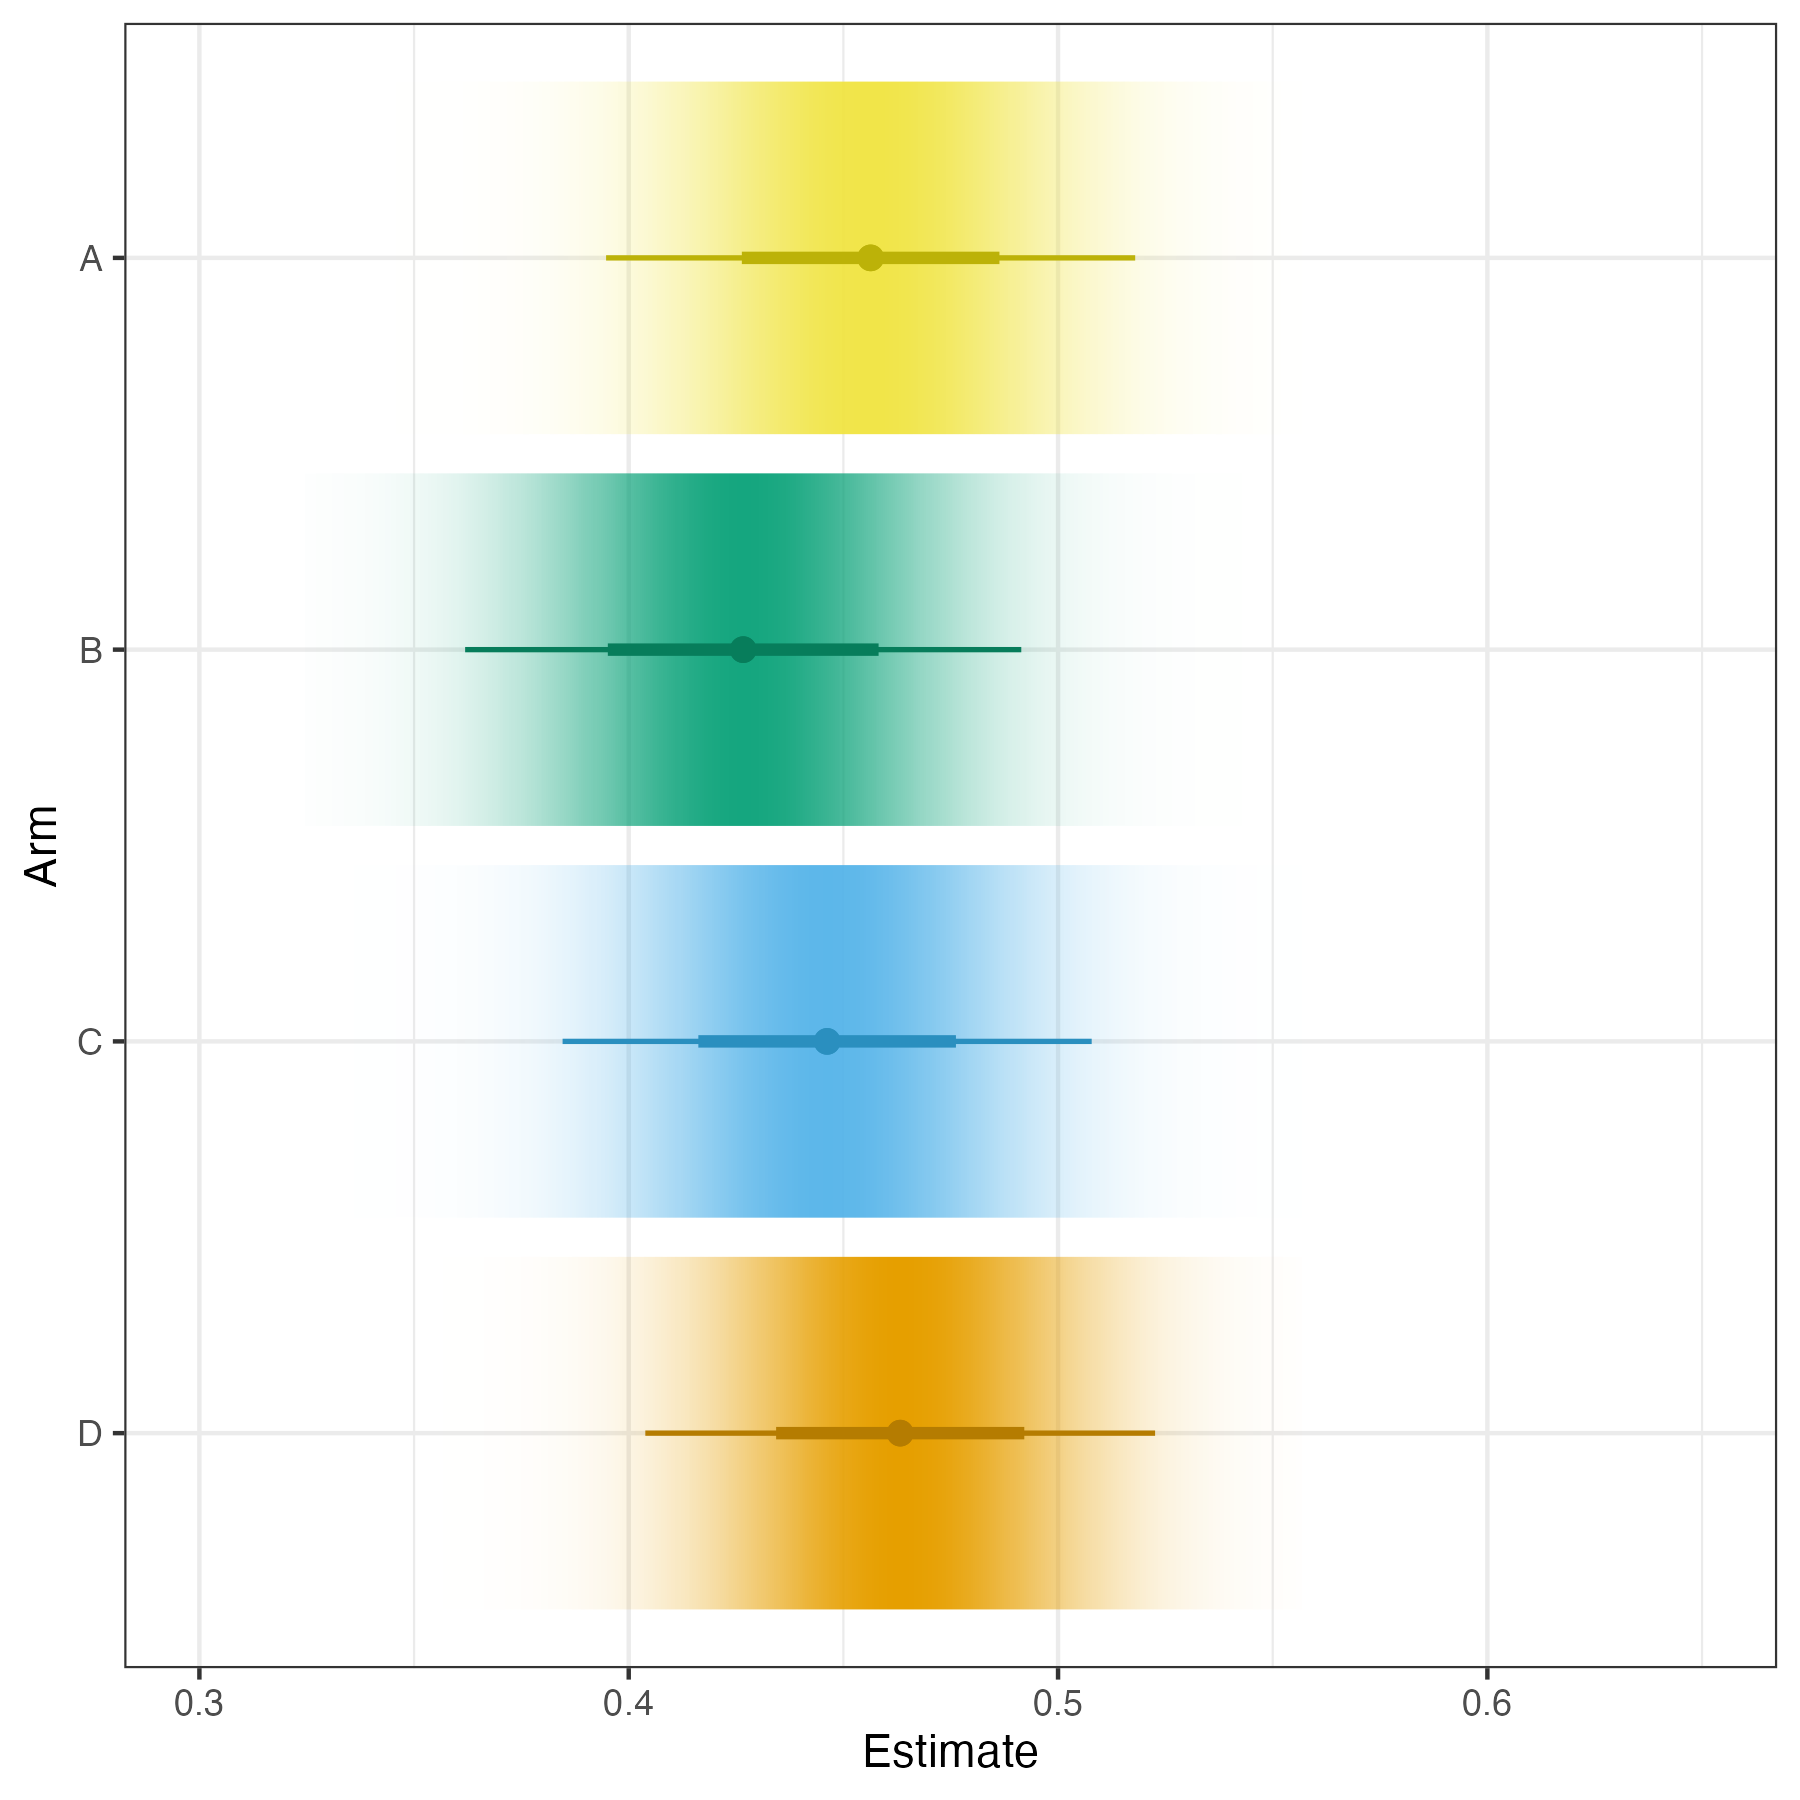
\includegraphics[width = 0.52\textwidth]{../assets/static_estimate4.png} \\
	\includegraphics[width = 1cm]{\figpath tv-ad.png} & \textbf B &\\
	\includegraphics[width = 1cm]{\figpath tv-ad.png} & \textbf C &\\
	\includegraphics[width = 1cm]{\figpath tv-ad.png} & \textbf D &\\ \vspace*{-30em} \ \\
    \end{tblr}
 };
\onslide<2>{\node at(a.center)[draw, red,line width=3pt,ellipse, minimum width=80pt, minimum height=50pt,rotate=0pt,yshift=-60pt, xshift = 43pt]{};}
\end{tikzpicture}   
\end{center}

\end{frame}


%%%%%NOTE%%%%%
\note{
\scriptsize \singlespacing
\begin{wideitemize}
\item You have an idea about different approaches to voter registration programs 
\item Question: you want to get an estimate of response under the \textit{best} treatment 
\item You design an experiment to test four of these
\item After the first phase of the experiment, you find two of the treatments perform well, but you are not able to distinguish between the two of them
\item You design a second stage of the experiment as a runoff between the two best-performing arms
\item You are able to get a precise estimate of response under the best treatment
\item We're dealing with the exploratory/confirmatory integration here. We could have just kept on running the first phase until we were able to get precise estimates of all of the arms, but it would have taken a larger, more expensive sample to get as precise an estimate of the best arm
\item Wasteful
\end{wideitemize}

}
%-------------------------------------------------------------------------------%
\begin{frame}[c]

\Large

\centering
\textcolor{Maroon}{Did we answer our research question?}

\end{frame}


%%%%%NOTE%%%%%
\note{
\scriptsize \singlespacing

%\begin{wideitemize}
%\item xxx
%\end{wideitemize}
}
%-------------------------------------------------------------------------------%
\begin{frame}{Framework}

\begin{wideitemize}
\item Individuals indexed $i = 1, \dots, n$\pause
\item Treatments $W_i \in \ww$, where $|\ww| = k$\pause
\item Potential outcome $Y_i = Y_i(W_i) \in \RR$; \\ 
        vector of potential outcomes  $\Y_i = (Y_i(1), \dots, Y_i(k))$%\pause
%\item Covariates $\X_i \in \RR^p$ \pause (Also: ``context'')
\item i.i.d. $\Y_i$
\end{wideitemize}

\end{frame}


%%%%%NOTE%%%%%
\note{
\scriptsize \singlespacing

%\begin{wideitemize}
%\item xxx
%\end{wideitemize}
}
%-------------------------------------------------------------------------------%
\begin{frame}{Evaluation metric}

Best arm:
\begin{equation*}
w^* \coloneqq \underset{w}{\argmax}\  \E[Y_i(w)].
\label{eq:best_arm}
\end{equation*}
\pause
In practice, we select $\hat w$ based on our allocation and recommendation procedures. \pause
\ \\
\ \\
Evaluate: 
\begin{equation*}
\E[ \hat w = w^*].
\label{eq:evaluate_best_arm}
\end{equation*}

\end{frame}


%%%%%NOTE%%%%%
\note{
\scriptsize \singlespacing

%\begin{wideitemize}
%\item xxx
%\end{wideitemize}
}
%-------------------------------------------------------------------------------%
\begin{frame}{Evaluation metric}

\begin{figure}[htbp] %  figure placement: here, top, bottom, or page
   \centering
   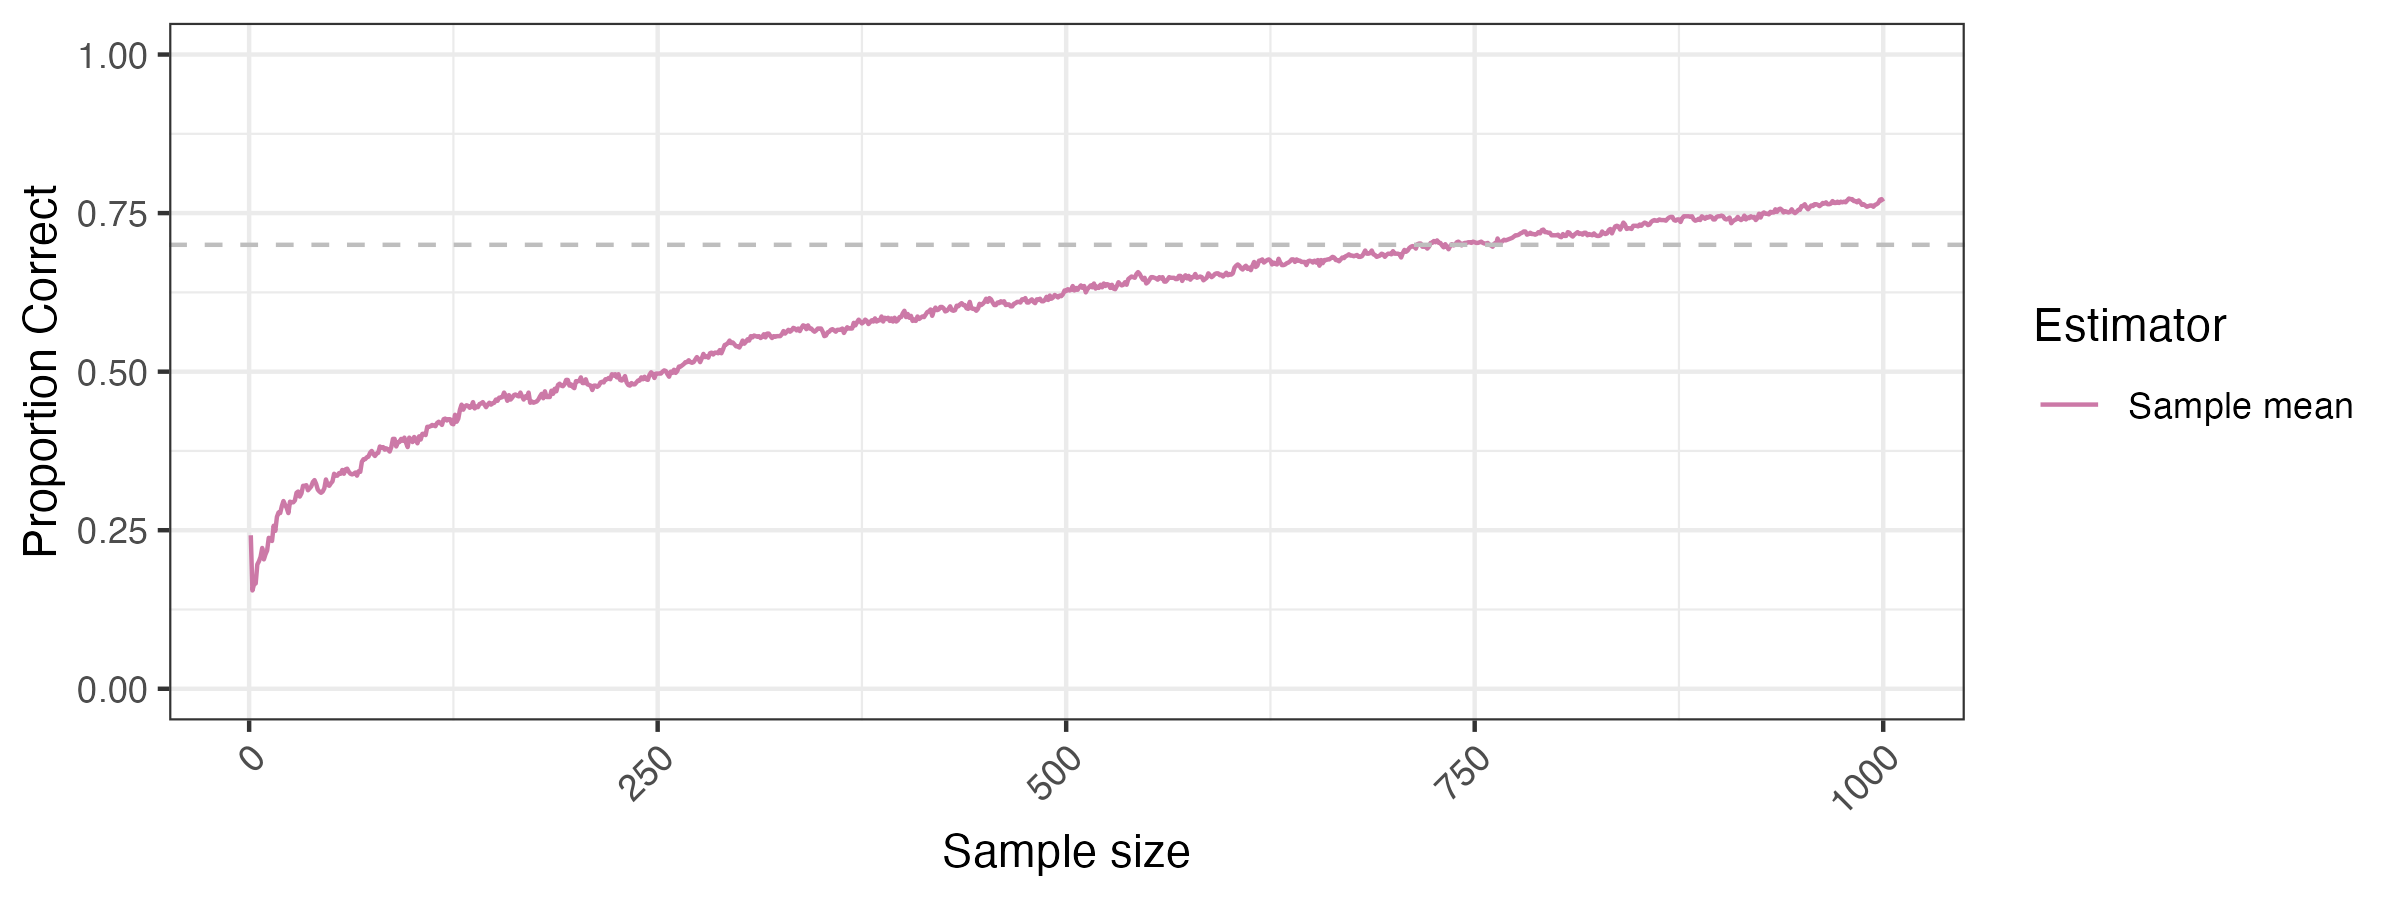
\includegraphics[width=\textwidth] {../assets/static_correct4.png} 
\end{figure}

\end{frame}


%%%%%NOTE%%%%%
\note{
\scriptsize \singlespacing
Things to note:
\begin{wideitemize}
\item We trade off which arm we think is best
\end{wideitemize}
}

%-------------------------------------------------------------------------------%
\begin{frame}{Can we better allocate our data?}

\begin{center}
\begin{tikzpicture}
\node(a){
\footnotesize
    \begin{tblr}{
    colspec={M{1.2cm}M{1cm}M{6cm}},row{2-5}={7ex},
      cells={halign=c, valign = m},
      stretch = 3
      }
      \SetCell[c=2]{} Advertisements &&  {Estimated \\ mean response}  \\
	 \includegraphics[width = 1cm]{\figpath tv-ad.png} & \textbf A & \SetCell[r=5]{c} \vspace*{-6em} 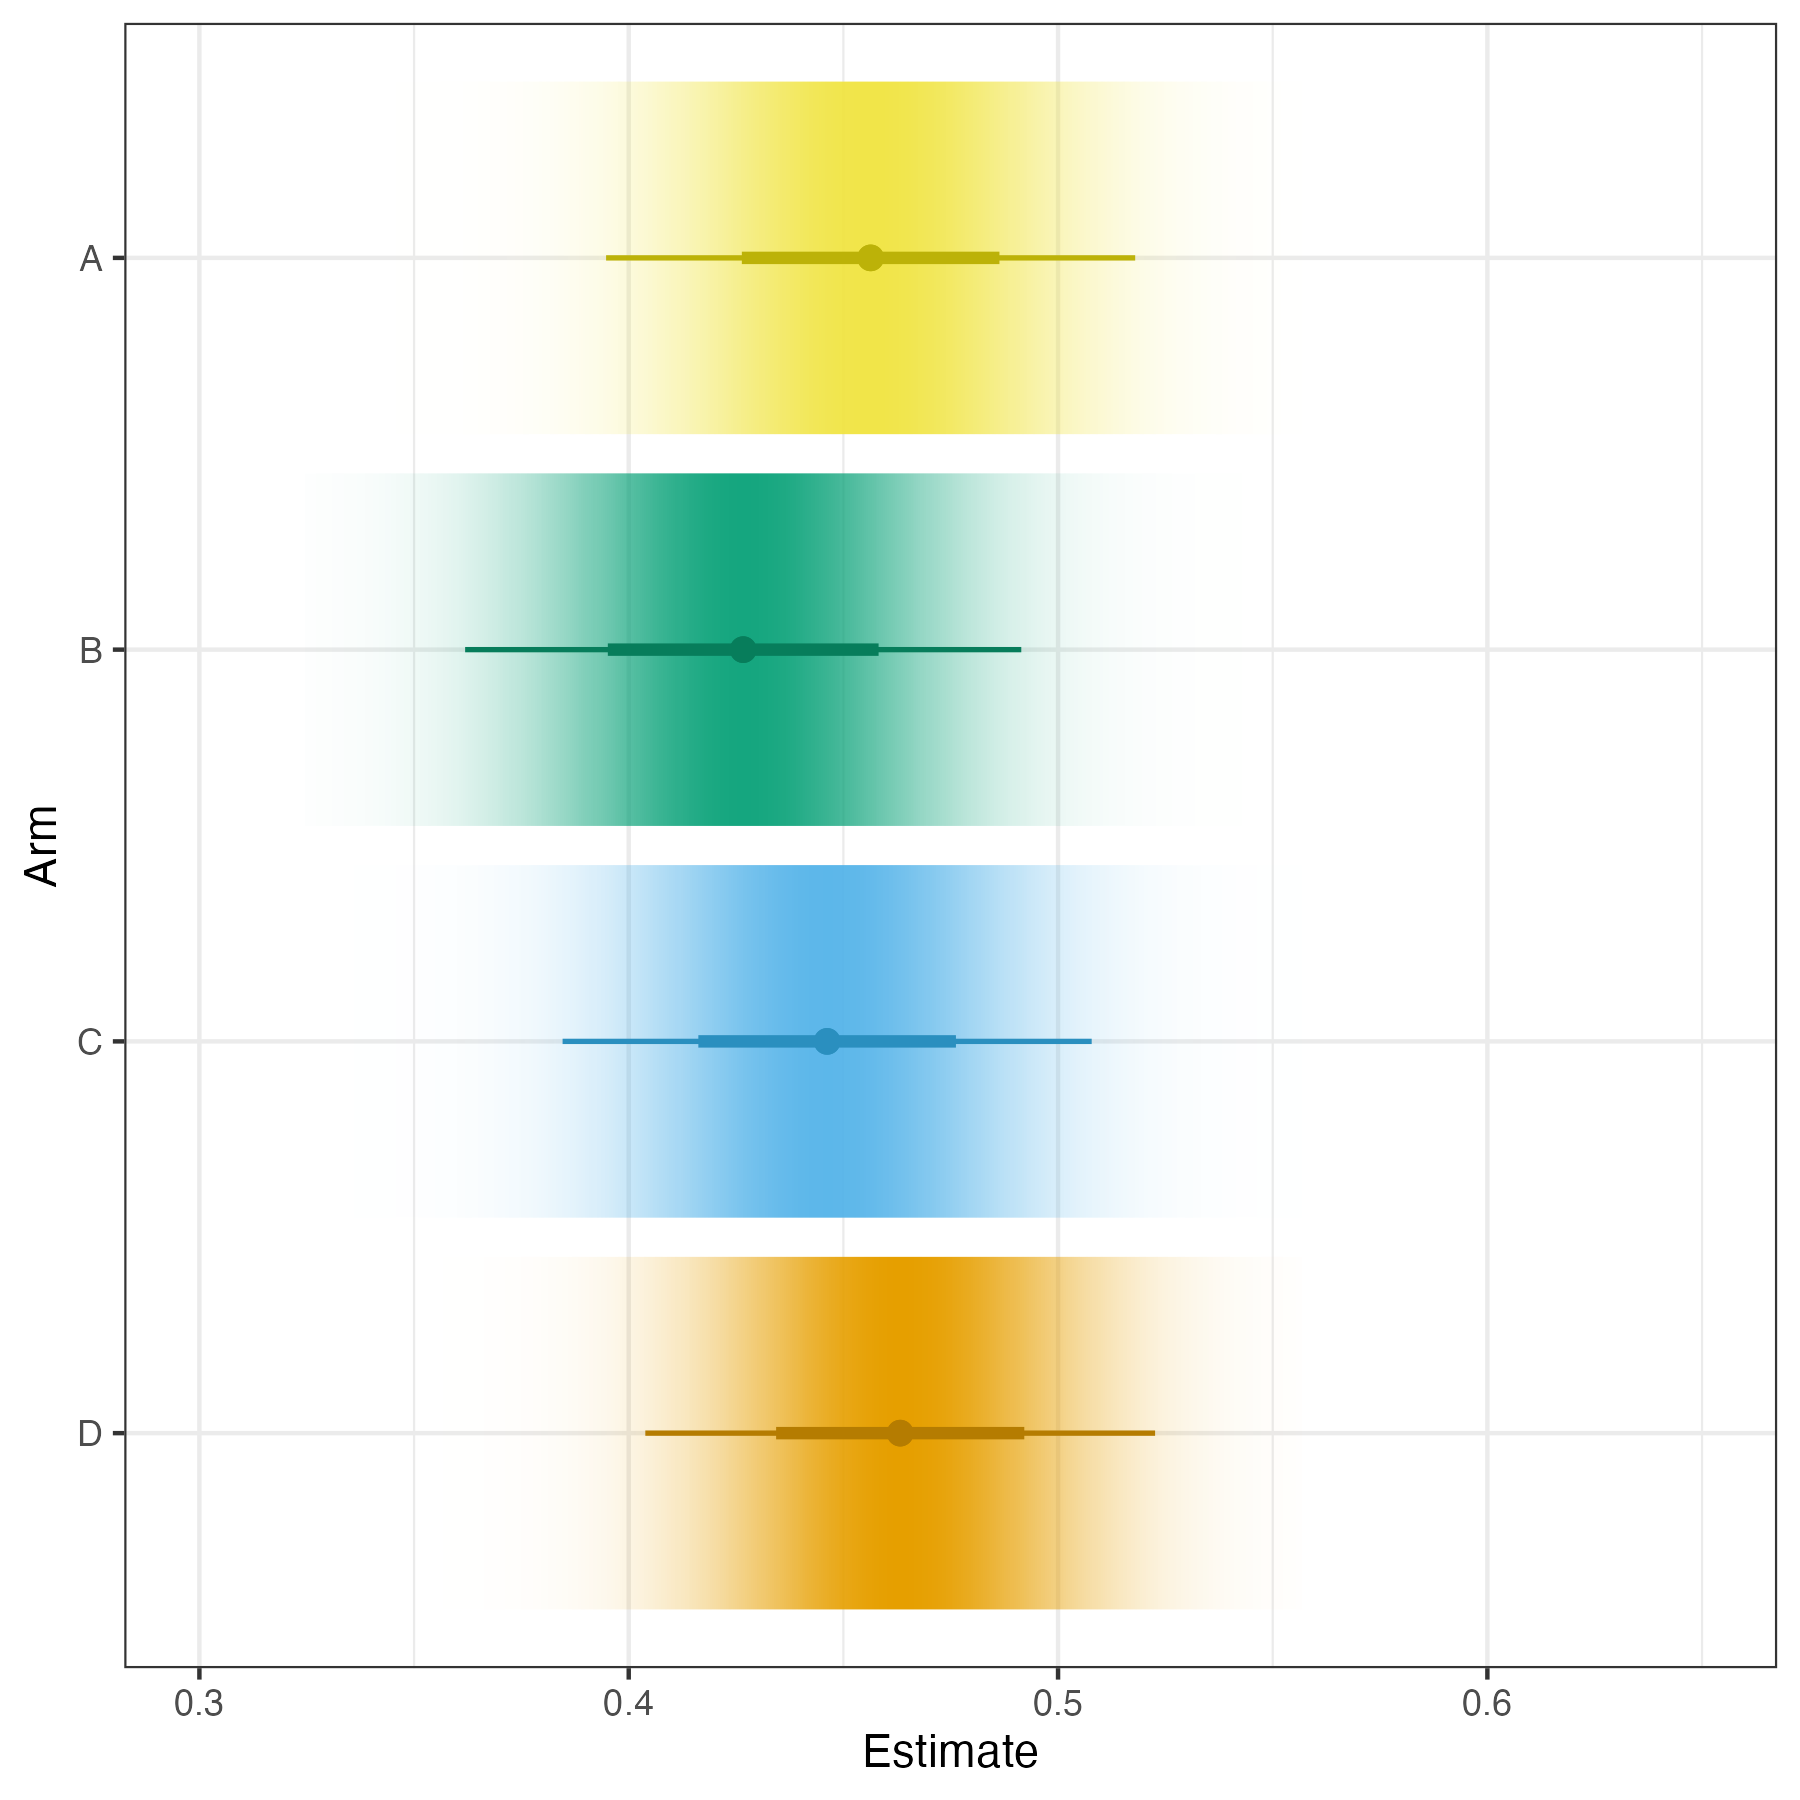
\includegraphics[width = 0.52\textwidth] {../assets/static_estimate4.png} \\
	\includegraphics[width = 1cm]{\figpath tv-ad.png} & \textbf B &\\
	\includegraphics[width = 1cm]{\figpath tv-ad.png} & \textbf C &\\
	\includegraphics[width = 1cm]{\figpath tv-ad.png} & \textbf D &\\ \vspace*{-30em} \ \\
    \end{tblr}
 };
%\onslide<2>{\node at(a.center)[draw, red,line width=3pt,ellipse, minimum width=80pt, minimum height=50pt,rotate=0pt,yshift=-60pt, xshift = 80pt]{};}
\end{tikzpicture}   
\end{center}

\end{frame}



%%%%%NOTE%%%%%
\note{
\scriptsize \singlespacing

%\begin{wideitemize}
%\item xxx
%\end{wideitemize}

}
%-------------------------------------------------------------------------------%
\begin{frame}{Response adaptive allocation}

\begin{figure}[htbp] %  figure placement: here, top, bottom, or page
   \centering
   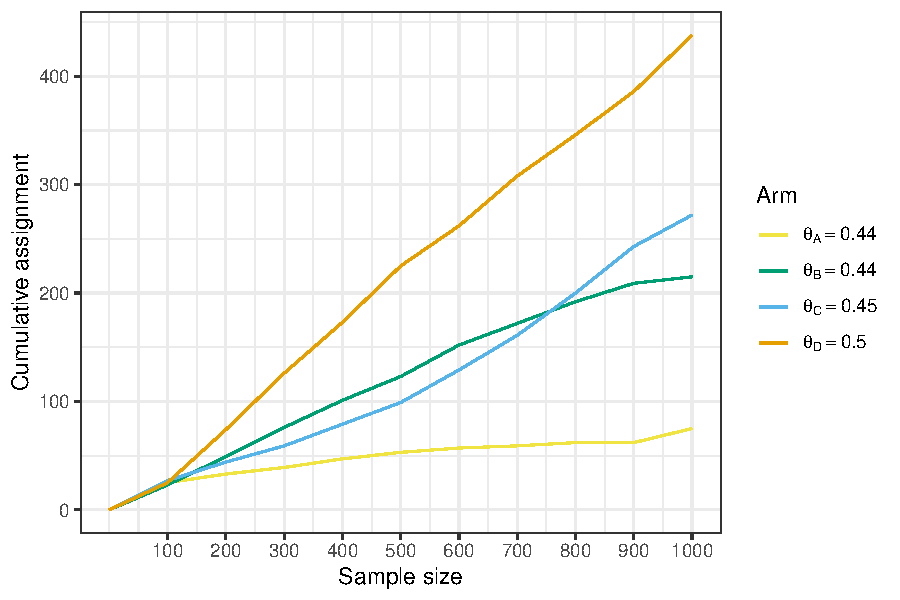
\includegraphics[width=.8\textwidth]{toyTTTS.pdf} 
\end{figure}

\end{frame}


%%%%%NOTE%%%%%
\note{
\scriptsize \singlespacing
Things to note:
\begin{wideitemize}
\item We trade off which arm we think is best
\end{wideitemize}
}

%-------------------------------------------------------------------------------%
\begin{frame}{Response adaptive allocation}

\begin{center}
\begin{tikzpicture}
\node(a){
\footnotesize
    \begin{tblr}{
    colspec={M{1.2cm}M{1cm}M{6cm}},row{2-5}={7ex},
      cells={halign=c, valign = m},
      stretch = 3
      }
      \SetCell[c=2]{} Advertisements &&  {Estimated \\ mean response}  \\
	 \includegraphics[width = 1cm]{\figpath tv-ad.png} & \textbf A & \SetCell[r=5]{c} \vspace*{-6em} 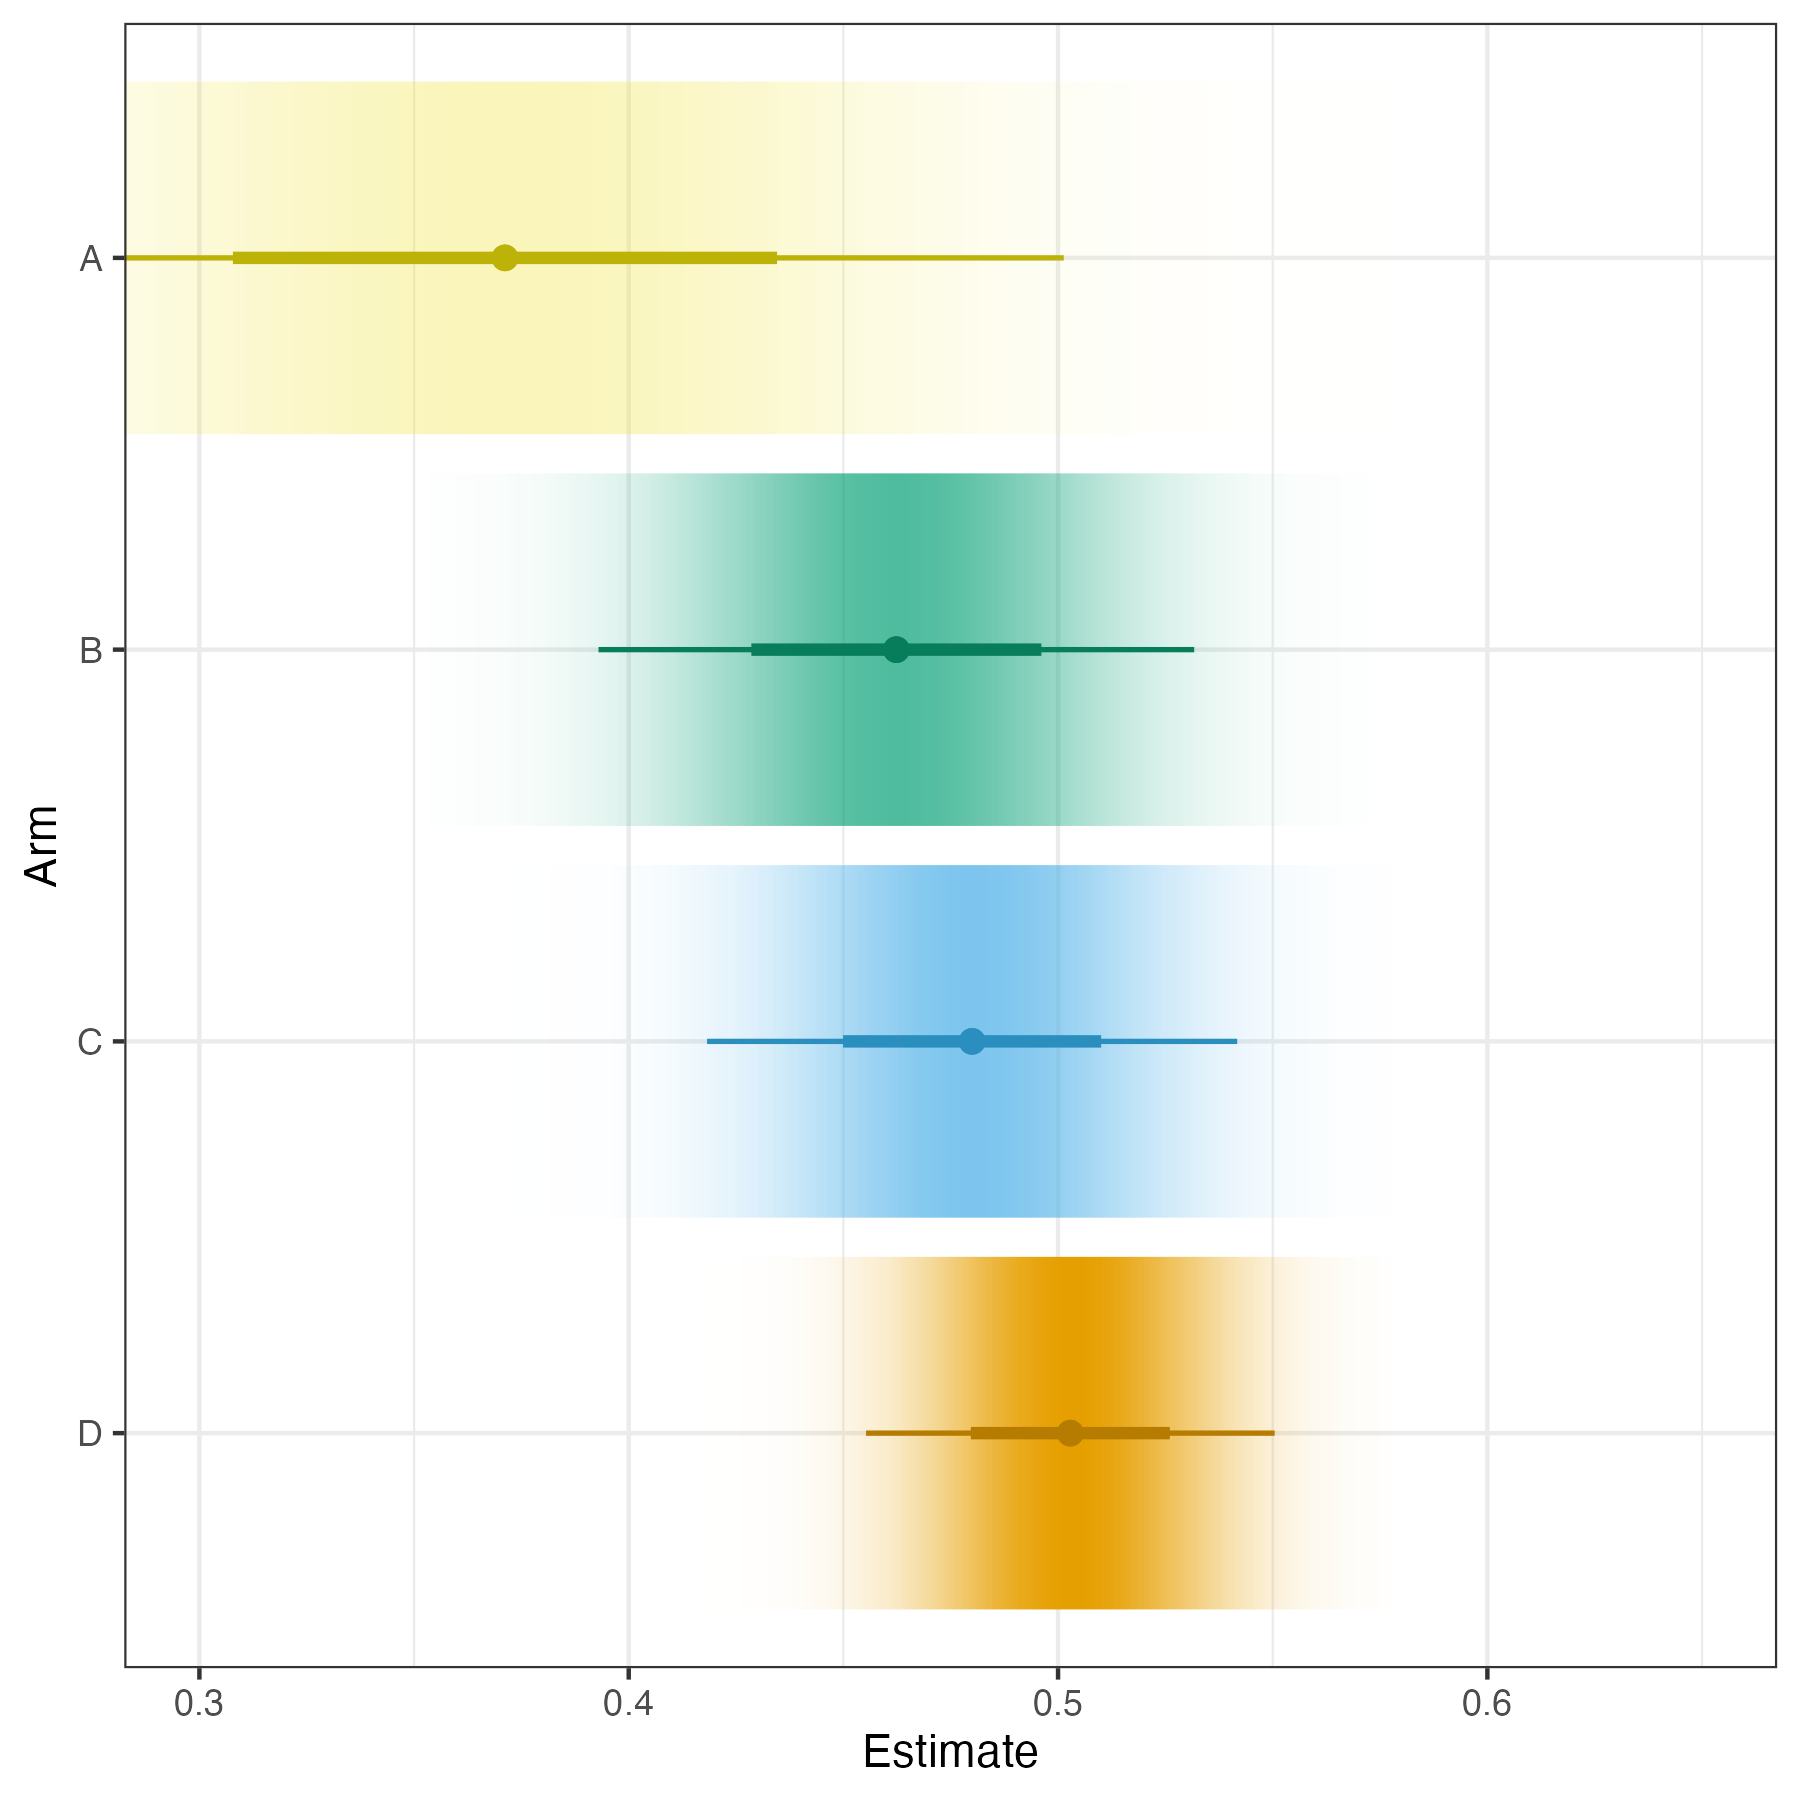
\includegraphics[width = 0.52\textwidth] {../assets/ttts_estimate4.png} \\
	\includegraphics[width = 1cm]{\figpath tv-ad.png} & \textbf B &\\
	\includegraphics[width = 1cm]{\figpath tv-ad.png} & \textbf C &\\
	\includegraphics[width = 1cm]{\figpath tv-ad.png} & \textbf D &\\ \vspace*{-30em} \ \\
    \end{tblr}
 };
%\onslide<2>{\node at(a.center)[draw, red,line width=3pt,ellipse, minimum width=80pt, minimum height=50pt,rotate=0pt,yshift=-60pt, xshift = 80pt]{};}
\end{tikzpicture}   
\end{center}

\end{frame}



%%%%%NOTE%%%%%
\note{
\scriptsize \singlespacing

%\begin{wideitemize}
%\item xxx
%\end{wideitemize}

}
%-------------------------------------------------------------------------------%
%\begin{frame}{Framework}
%
%\begin{wideitemize}
%\item Individuals indexed $i = 1, \dots, n$
%\item Treatments $W_i \in \ww$, where $|\ww| = k$
%\item Potential outcome $Y_i = Y_i(W_i) \in \RR$; \\ 
%        vector of potential outcomes  $\Y_i \coloneqq (Y_i(1), \dots, Y_i(k))$
%\item \textcolor{lightgray}{Covariates $\X_i \in \RR^p$  (Also: ``context'')} 
%\item i.i.d. $(\Y_i, \textcolor{lightgray}{\X_i} )$
%\end{wideitemize}
%
%\end{frame}
%
%
%%%%%%NOTE%%%%%
%\note{
%\scriptsize \singlespacing
%
%%\begin{wideitemize}
%%\item xxx
%%\end{wideitemize}
%}
%%-------------------------------------------------------------------------------%
\begin{frame}{Framework}

\begin{wideitemize}
\item Account for some \textbf{history} at time we see individual $i$: 
\[
\HB_i=
  \begin{bmatrix}
    Y_1 & W_1 & \textcolor{lightgray}{X_{[1]1}} & \textcolor{lightgray}{\hdots} & \textcolor{lightgray}{X_{[1]p}} \\
    Y_2 & W_2 &  \textcolor{lightgray}{X_{[2]1}} & \textcolor{lightgray}{\hdots} & \textcolor{lightgray}{X_{[2]p}} \\
    \textcolor{lightgray}{\vdots} & & & & \textcolor{lightgray}{\vdots} \\
    Y_{i-1} & W_{i-1}&  \textcolor{lightgray}{X_{[i-1]1}} & \textcolor{lightgray}{\hdots} &  \textcolor{lightgray}{X_{[i-1]p}} \\
%    \textcolor{lightgray}{?} & \textcolor{lightgray}{?} & X_{[i]1}& \hdots & X_{[i]p} \\
    \textcolor{lightgray}{\vdots} & & & & \textcolor{lightgray}{\vdots} \\
    \textcolor{lightgray}{?} & \textcolor{lightgray}{?} & \textcolor{lightgray}{?} & \textcolor{lightgray}{\hdots} & \textcolor{lightgray}{?} 
  \end{bmatrix}
\]
\pause
\item We don't assume the whole sampling frame is known. 
\end{wideitemize}

\end{frame}


%%%%%NOTE%%%%%
\note{
\scriptsize \singlespacing

%\begin{wideitemize}
%\item xxx
%\end{wideitemize}
}
%-------------------------------------------------------------------------------%
\begin{frame}{Framework}

\begin{wideitemize}
\item Treatment assignment probability
\begin{equation*}
\begin{split}
e_i(w)\coloneqq  \Pr\left[{W_i = w \textcolor{lightgray}{|\X_i = x}}\right]\\
\e \coloneqq (e(1), \dots, e(k))
%\sum_{w}e_i(w) = 1
\end{split}
\end{equation*}\pause
\item \textbf{Policy}
\begin{equation*}
\pi : \HB\textcolor{lightgray}{, \X} \rightarrow \e\text, 
\end{equation*} \pause
\begin{itemize}
\item Constrained by a policy class $\Pi$ \pause \\
(functional form, cost constraints in assignment probabilities)
\end{itemize}
\end{wideitemize}

\end{frame}


%%%%%NOTE%%%%%
\note{
\scriptsize \singlespacing

%\begin{wideitemize}
%\item xxx
%\end{wideitemize}
}
%-------------------------------------------------------------------------------%

\begin{frame}{Thompson sampling}
\scriptsize

\onslide<2- 6>
\textbf{Setup:} Multiple treatment arms. Start with uniform priors.

\onslide<3-6>
 \textbf{Timepoint 1:} 
\begin{itemize}
\item Assign treatment uniformly at random. 
\item Observe response. 
\item Update posterior distributions based on observed data.
\item Calculate posterior probability that each arm is best. %, i.e., $P\left(\mu_1 \ge \mu_2, \dots, \mu_w \right | \textrm{prior, data} )$
\end{itemize}

\onslide<4-6>
 \textbf{Timepoint 2:} 
\begin{itemize}
\item \onslide<4->\only<7>{ \textcolor{structure}}{Assign treatment according to posterior probability that each arm is best.}
\onslide<4-6>
\item Observe response. 
\item Update posterior distributions based on the observed data. 
\item Calculate posterior probability that each arm is best.\\
\end{itemize}

\onslide<5-6>
\hspace{15 pt} $\vdots$\\
Repeat actions from batch 2. \\
\hspace{15 pt} $\vdots$\\
\onslide<6>
 \textbf{Stopping rule} 

\onslide<7>\hyperlink{ts}{\beamerbutton{Thompson sampling}}\hypertarget<7>{ts-explainer}{}
\end{frame}


%%%%%NOTE%%%%%
\note{
\scriptsize \singlespacing
\begin{wideitemize}
%\item the question is how you choose a strategy for selecting $n_t$ arms
\item TS one of the oldest and most widely studied approaches to adaptive design, and, as far as I know, what's being used widely in tech industry\\
$\rightarrow$ explain algorithm
\item TS is a decision-theoretic, heuristic approach: gives you info on what to do next\\
\item NOT guaranteed to pick the best arm $\rightarrow$ but performs well in practice
\item And helps navigate the explore/exploit tradeoff: you get enough information about bad arms to know they're not good
\item then want to spend time figuring out, among good arms, which one is truly best. It performs well on each of the objectives outlined above \textcolor{red}{[citations]}. 
\item for probability each arm is optimal--simulate samples, or calculate by quadrature
\item Repeat until stopping rule: \% prob best, or set num periods
\item This is the standard Bayesian approach. In Susan Athey's lab, we're using a frequentist hybrid, where you estimate the mean and variance, assume a normal distribution, and draw from that, but the treatment assignment probability step is very similar
\end{wideitemize}
}
%-------------------------------------------------------------------------------%
\begin{frame}

\vspace*{-1pt}
\makebox[\linewidth]{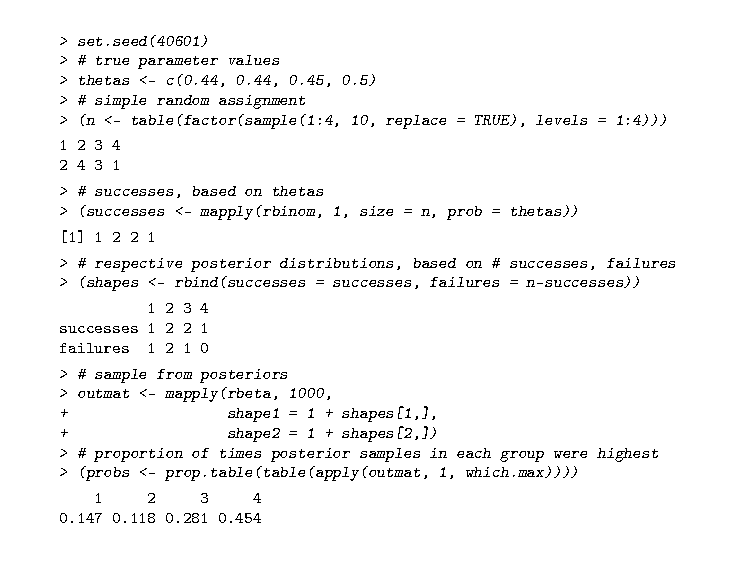
\includegraphics[page=1,width=\paperwidth]{TS.pdf}}

\end{frame}


%%%%%NOTE%%%%%
\note{
\scriptsize \singlespacing

%\begin{wideitemize}
%\item xxx
%\end{wideitemize}
}
%-------------------------------------------------------------------------------%
\begin{frame}{Policies: response adaptive allocation}

\begin{equation*}
\pi : \HB\textcolor{lightgray}{, X} \rightarrow \e 
\end{equation*}

Examples of policies: 
Response-adaptive allocation

\only<1>{
\begin{table}[]
\begin{tabular}{c cccc | ccc}
 &  &  & & & \multicolumn{3}{c}{$\HB_i$} \\
 Unit & $e_i(A)$ & $e_i(B)$ & $e_i(C)$ & $e_i(D)$ &  {$Y_{i}$} & {$W_{i}$} & \textcolor{lightgray}{$X_{[i]1}$}  \\
 \hline
1 & \num{0.25} & \num{0.25} & \num{0.25} & \num{0.25} & \textcolor{lightgray}{?} & \textcolor{lightgray}{?} & \textcolor{lightgray}{?} \\
2 & \textcolor{lightgray}{?} & \textcolor{lightgray}{?} & \textcolor{lightgray}{?} & \textcolor{lightgray}{?} & \textcolor{lightgray}{?} & \textcolor{lightgray}{?} & \textcolor{lightgray}{?} \\
3 & \textcolor{lightgray}{?} & \textcolor{lightgray}{?} & \textcolor{lightgray}{?} & \textcolor{lightgray}{?} & \textcolor{lightgray}{?} & \textcolor{lightgray}{?} & \textcolor{lightgray}{?} \\
4 & \textcolor{lightgray}{?} & \textcolor{lightgray}{?} & \textcolor{lightgray}{?} & \textcolor{lightgray}{?} & \textcolor{lightgray}{?} & \textcolor{lightgray}{?} & \textcolor{lightgray}{?} \\
5 & \textcolor{lightgray}{?} & \textcolor{lightgray}{?} & \textcolor{lightgray}{?} &\textcolor{lightgray}{?} & \textcolor{lightgray}{?} & \textcolor{lightgray}{?} & \textcolor{lightgray}{?} \\
6 & \textcolor{lightgray}{?} & \textcolor{lightgray}{?} & \textcolor{lightgray}{?} & \textcolor{lightgray}{?} & \textcolor{lightgray}{?} & \textcolor{lightgray}{?} & \textcolor{lightgray}{?} 
\end{tabular}
\end{table}
}


\only<2>{
\begin{table}[]
\begin{tabular}{c cccc | ccc}
 &  &  & & & \multicolumn{3}{c}{$\HB_i$} \\
 Unit & $e_i(A)$ & $e_i(B)$ & $e_i(C)$ & $e_i(D)$ &  {$Y_{i}$} & {$W_{i}$} & \textcolor{lightgray}{$X_{[i]1}$}  \\
 \hline
1 & \num{0.25} & \num{0.25} & \num{0.25} & \num{0.25} & \textcolor{lightgray}{?} & D & \textcolor{lightgray}{?} \\
2 & \textcolor{lightgray}{?} & \textcolor{lightgray}{?} & \textcolor{lightgray}{?} & \textcolor{lightgray}{?} & \textcolor{lightgray}{?} & \textcolor{lightgray}{?} & \textcolor{lightgray}{?} \\
3 & \textcolor{lightgray}{?} & \textcolor{lightgray}{?} & \textcolor{lightgray}{?} & \textcolor{lightgray}{?} & \textcolor{lightgray}{?} & \textcolor{lightgray}{?} & \textcolor{lightgray}{?} \\
4 & \textcolor{lightgray}{?} & \textcolor{lightgray}{?} & \textcolor{lightgray}{?} & \textcolor{lightgray}{?} & \textcolor{lightgray}{?} & \textcolor{lightgray}{?} & \textcolor{lightgray}{?} \\
5 & \textcolor{lightgray}{?} & \textcolor{lightgray}{?} & \textcolor{lightgray}{?} &\textcolor{lightgray}{?} & \textcolor{lightgray}{?} & \textcolor{lightgray}{?} & \textcolor{lightgray}{?} \\
6 & \textcolor{lightgray}{?} & \textcolor{lightgray}{?} & \textcolor{lightgray}{?} & \textcolor{lightgray}{?} & \textcolor{lightgray}{?} & \textcolor{lightgray}{?} & \textcolor{lightgray}{?} 
\end{tabular}
\end{table}
}

\only<3>{
\begin{table}[]
\begin{tabular}{c cccc | ccc}
 &  &  & & & \multicolumn{3}{c}{$\HB_i$} \\
 Unit & $e_i(A)$ & $e_i(B)$ & $e_i(C)$ & $e_i(D)$ &  {$Y_{i}$} & {$W_{i}$} & \textcolor{lightgray}{$X_{[i]1}$}  \\
 \hline
1 & \num{0.25} & \num{0.25} & \num{0.25} & \num{0.25} &0 & D & \textcolor{lightgray}{?} \\
2 & \textcolor{lightgray}{?} & \textcolor{lightgray}{?} & \textcolor{lightgray}{?} & \textcolor{lightgray}{?} & \textcolor{lightgray}{?} & \textcolor{lightgray}{?} & \textcolor{lightgray}{?} \\
3 & \textcolor{lightgray}{?} & \textcolor{lightgray}{?} & \textcolor{lightgray}{?} & \textcolor{lightgray}{?} & \textcolor{lightgray}{?} & \textcolor{lightgray}{?} & \textcolor{lightgray}{?} \\
4 & \textcolor{lightgray}{?} & \textcolor{lightgray}{?} & \textcolor{lightgray}{?} & \textcolor{lightgray}{?} & \textcolor{lightgray}{?} & \textcolor{lightgray}{?} & \textcolor{lightgray}{?} \\
5 & \textcolor{lightgray}{?} & \textcolor{lightgray}{?} & \textcolor{lightgray}{?} &\textcolor{lightgray}{?} & \textcolor{lightgray}{?} & \textcolor{lightgray}{?} & \textcolor{lightgray}{?} \\
6 & \textcolor{lightgray}{?} & \textcolor{lightgray}{?} & \textcolor{lightgray}{?} & \textcolor{lightgray}{?} & \textcolor{lightgray}{?} & \textcolor{lightgray}{?} & \textcolor{lightgray}{?} 
\end{tabular}
\end{table}
}


\end{frame}


%%%%%NOTE%%%%%
\note{
\scriptsize \singlespacing

%\begin{wideitemize}
%\item xxx
%\end{wideitemize}
}
%-------------------------------------------------------------------------------%




\begin{frame}{Policies: response adaptive allocation}

\begin{equation*}
\pi : \HB\textcolor{lightgray}{, X} \rightarrow \e 
\end{equation*}

Examples of policies: 
Response-adaptive allocation

\only<1>{
\begin{table}[]
\begin{tabular}{c cccc | ccc}
 &  &  & & & \multicolumn{3}{c}{$\HB_i$} \\
 Unit & $e_i(A)$ & $e_i(B)$ & $e_i(C)$ & $e_i(D)$ &  {$Y_{i}$} & {$W_{i}$} & \textcolor{lightgray}{$X_{[i]1}$}  \\
 \hline
1 & \num{0.25} & \num{0.25} & \num{0.25} & \num{0.25} &0 & D & \textcolor{lightgray}{?} \\
2 & \num{0.30} & \num{0.30} & \num{0.30} & \num{0.10} & \textcolor{lightgray}{?} & \textcolor{lightgray}{?} & \textcolor{lightgray}{?}  \\
3 & \textcolor{lightgray}{?} & \textcolor{lightgray}{?} & \textcolor{lightgray}{?} & \textcolor{lightgray}{?} & \textcolor{lightgray}{?} & \textcolor{lightgray}{?} & \textcolor{lightgray}{?} \\
4 & \textcolor{lightgray}{?} & \textcolor{lightgray}{?} & \textcolor{lightgray}{?} & \textcolor{lightgray}{?} & \textcolor{lightgray}{?} & \textcolor{lightgray}{?} & \textcolor{lightgray}{?} \\
5 & \textcolor{lightgray}{?} & \textcolor{lightgray}{?} & \textcolor{lightgray}{?} &\textcolor{lightgray}{?} & \textcolor{lightgray}{?} & \textcolor{lightgray}{?} & \textcolor{lightgray}{?} \\
6 & \textcolor{lightgray}{?} & \textcolor{lightgray}{?} & \textcolor{lightgray}{?} & \textcolor{lightgray}{?} & \textcolor{lightgray}{?} & \textcolor{lightgray}{?} & \textcolor{lightgray}{?} 
\end{tabular}
\end{table}
}


\only<2>{
\begin{table}[]
\begin{tabular}{c cccc | ccc}
 &  &  & & & \multicolumn{3}{c}{$\HB_i$} \\
 Unit & $e_i(A)$ & $e_i(B)$ & $e_i(C)$ & $e_i(D)$ &  {$Y_{i}$} & {$W_{i}$} & \textcolor{lightgray}{$X_{[i]1}$}  \\
 \hline
1 & \num{0.25} & \num{0.25} & \num{0.25} & \num{0.25} &0 & D & \textcolor{lightgray}{?} \\
2 & \num{0.30} & \num{0.30} & \num{0.30} & \num{0.10} & \textcolor{lightgray}{?} & D & \textcolor{lightgray}{?}  \\
3 & \textcolor{lightgray}{?} & \textcolor{lightgray}{?} & \textcolor{lightgray}{?} & \textcolor{lightgray}{?} & \textcolor{lightgray}{?} & \textcolor{lightgray}{?} & \textcolor{lightgray}{?} \\
4 & \textcolor{lightgray}{?} & \textcolor{lightgray}{?} & \textcolor{lightgray}{?} & \textcolor{lightgray}{?} & \textcolor{lightgray}{?} & \textcolor{lightgray}{?} & \textcolor{lightgray}{?} \\
5 & \textcolor{lightgray}{?} & \textcolor{lightgray}{?} & \textcolor{lightgray}{?} &\textcolor{lightgray}{?} & \textcolor{lightgray}{?} & \textcolor{lightgray}{?} & \textcolor{lightgray}{?} \\
6 & \textcolor{lightgray}{?} & \textcolor{lightgray}{?} & \textcolor{lightgray}{?} & \textcolor{lightgray}{?} & \textcolor{lightgray}{?} & \textcolor{lightgray}{?} & \textcolor{lightgray}{?} 
\end{tabular}
\end{table}
}

\only<3>{
\begin{table}[]
\begin{tabular}{c cccc | ccc}
 &  &  & & & \multicolumn{3}{c}{$\HB_i$} \\
 Unit & $e_i(A)$ & $e_i(B)$ & $e_i(C)$ & $e_i(D)$ &  {$Y_{i}$} & {$W_{i}$} & \textcolor{lightgray}{$X_{[i]1}$}  \\
 \hline
1 & \num{0.25} & \num{0.25} & \num{0.25} & \num{0.25} &0 & D & \textcolor{lightgray}{?} \\
2 & \num{0.30} & \num{0.30} & \num{0.30} & \num{0.10} & 1 & D & \textcolor{lightgray}{?}  \\
3 & \textcolor{lightgray}{?} & \textcolor{lightgray}{?} & \textcolor{lightgray}{?} & \textcolor{lightgray}{?} & \textcolor{lightgray}{?} & \textcolor{lightgray}{?} & \textcolor{lightgray}{?} \\
4 & \textcolor{lightgray}{?} & \textcolor{lightgray}{?} & \textcolor{lightgray}{?} & \textcolor{lightgray}{?} & \textcolor{lightgray}{?} & \textcolor{lightgray}{?} & \textcolor{lightgray}{?} \\
5 & \textcolor{lightgray}{?} & \textcolor{lightgray}{?} & \textcolor{lightgray}{?} &\textcolor{lightgray}{?} & \textcolor{lightgray}{?} & \textcolor{lightgray}{?} & \textcolor{lightgray}{?} \\
6 & \textcolor{lightgray}{?} & \textcolor{lightgray}{?} & \textcolor{lightgray}{?} & \textcolor{lightgray}{?} & \textcolor{lightgray}{?} & \textcolor{lightgray}{?} & \textcolor{lightgray}{?} 
\end{tabular}
\end{table}
}

\only<4>{
\begin{table}[]
\begin{tabular}{c cccc | ccc}
 &  &  & & & \multicolumn{3}{c}{$\HB_i$} \\
 Unit & $e_i(A)$ & $e_i(B)$ & $e_i(C)$ & $e_i(D)$ &  {$Y_{i}$} & {$W_{i}$} & \textcolor{lightgray}{$X_{[i]1}$}  \\
 \hline
1 & \num{0.25} & \num{0.25} & \num{0.25} & \num{0.25} &0 & D & \textcolor{lightgray}{?} \\
2 & \num{0.30} & \num{0.30} & \num{0.30} & \num{0.10} & 1 & D & \textcolor{lightgray}{?}  \\
3 & \num{0.27} & \num{0.26} & \num{0.27} & \num{0.20} & \textcolor{lightgray}{?} & \textcolor{lightgray}{?} & \textcolor{lightgray}{?} \\
4 & \textcolor{lightgray}{?} & \textcolor{lightgray}{?} & \textcolor{lightgray}{?} & \textcolor{lightgray}{?} & \textcolor{lightgray}{?} & \textcolor{lightgray}{?} & \textcolor{lightgray}{?} \\
5 & \textcolor{lightgray}{?} & \textcolor{lightgray}{?} & \textcolor{lightgray}{?} &\textcolor{lightgray}{?} & \textcolor{lightgray}{?} & \textcolor{lightgray}{?} & \textcolor{lightgray}{?} \\
6 & \textcolor{lightgray}{?} & \textcolor{lightgray}{?} & \textcolor{lightgray}{?} & \textcolor{lightgray}{?} & \textcolor{lightgray}{?} & \textcolor{lightgray}{?} & \textcolor{lightgray}{?} 
\end{tabular}
\end{table}
}

\only<5>{
\begin{table}[]
\begin{tabular}{c cccc | ccc}
 &  &  & & & \multicolumn{3}{c}{$\HB_i$} \\
 Unit & $e_i(A)$ & $e_i(B)$ & $e_i(C)$ & $e_i(D)$ &  {$Y_{i}$} & {$W_{i}$} & \textcolor{lightgray}{$X_{[i]1}$}  \\
 \hline
1 & \num{0.25} & \num{0.25} & \num{0.25} & \num{0.25} &0 & D & \textcolor{lightgray}{?} \\
2 & \num{0.30} & \num{0.30} & \num{0.30} & \num{0.10} & 1 & D & \textcolor{lightgray}{?}  \\
3 & \num{0.27} & \num{0.26} & \num{0.27} & \num{0.20} & \textcolor{lightgray}{?} & A & \textcolor{lightgray}{?} \\
4 & \textcolor{lightgray}{?} & \textcolor{lightgray}{?} & \textcolor{lightgray}{?} & \textcolor{lightgray}{?} & \textcolor{lightgray}{?} & \textcolor{lightgray}{?} & \textcolor{lightgray}{?} \\
5 & \textcolor{lightgray}{?} & \textcolor{lightgray}{?} & \textcolor{lightgray}{?} &\textcolor{lightgray}{?} & \textcolor{lightgray}{?} & \textcolor{lightgray}{?} & \textcolor{lightgray}{?} \\
6 & \textcolor{lightgray}{?} & \textcolor{lightgray}{?} & \textcolor{lightgray}{?} & \textcolor{lightgray}{?} & \textcolor{lightgray}{?} & \textcolor{lightgray}{?} & \textcolor{lightgray}{?} 
\end{tabular}
\end{table}
}


\only<6>{
\begin{table}[]
\begin{tabular}{c cccc | ccc}
 &  &  & & & \multicolumn{3}{c}{$\HB_i$} \\
 Unit & $e_i(A)$ & $e_i(B)$ & $e_i(C)$ & $e_i(D)$ &  {$Y_{i}$} & {$W_{i}$} & \textcolor{lightgray}{$X_{[i]1}$}  \\
 \hline
1 & \num{0.25} & \num{0.25} & \num{0.25} & \num{0.25} &0 & D & \textcolor{lightgray}{?} \\
2 & \num{0.30} & \num{0.30} & \num{0.30} & \num{0.10} & 1 & D & \textcolor{lightgray}{?}  \\
3 & \num{0.27} & \num{0.26} & \num{0.27} & \num{0.20} & 0 & A & \textcolor{lightgray}{?} \\
4 & \textcolor{lightgray}{?} & \textcolor{lightgray}{?} & \textcolor{lightgray}{?} & \textcolor{lightgray}{?} & \textcolor{lightgray}{?} & \textcolor{lightgray}{?} & \textcolor{lightgray}{?} \\
5 & \textcolor{lightgray}{?} & \textcolor{lightgray}{?} & \textcolor{lightgray}{?} &\textcolor{lightgray}{?} & \textcolor{lightgray}{?} & \textcolor{lightgray}{?} & \textcolor{lightgray}{?} \\
6 & \textcolor{lightgray}{?} & \textcolor{lightgray}{?} & \textcolor{lightgray}{?} & \textcolor{lightgray}{?} & \textcolor{lightgray}{?} & \textcolor{lightgray}{?} & \textcolor{lightgray}{?} 
\end{tabular}
\end{table}
}

\only<7>{
\begin{table}[]
\begin{tabular}{c cccc | ccc}
 &  &  & & & \multicolumn{3}{c}{$\HB_i$} \\
 Unit & $e_i(A)$ & $e_i(B)$ & $e_i(C)$ & $e_i(D)$ &  {$Y_{i}$} & {$W_{i}$} & \textcolor{lightgray}{$X_{[i]1}$}  \\
 \hline
1 & \num{0.25} & \num{0.25} & \num{0.25} & \num{0.25} &0 & D & \textcolor{lightgray}{?} \\
2 & \num{0.30} & \num{0.30} & \num{0.30} & \num{0.10} & 1 & D & \textcolor{lightgray}{?}  \\
3 & \num{0.27} & \num{0.26} & \num{0.27} & \num{0.20} & 0 & A & \textcolor{lightgray}{?} \\
4 & \num{0.11} & \num{0.32} & \num{0.32} & \num{0.26} & \textcolor{lightgray}{?} & \textcolor{lightgray}{?} & \textcolor{lightgray}{?} \\
5 & \textcolor{lightgray}{?} & \textcolor{lightgray}{?} & \textcolor{lightgray}{?} &\textcolor{lightgray}{?} & \textcolor{lightgray}{?} & \textcolor{lightgray}{?} & \textcolor{lightgray}{?} \\
6 & \textcolor{lightgray}{?} & \textcolor{lightgray}{?} & \textcolor{lightgray}{?} & \textcolor{lightgray}{?} & \textcolor{lightgray}{?} & \textcolor{lightgray}{?} & \textcolor{lightgray}{?} 
\end{tabular}
\end{table}
}

\only<8>{
\begin{table}[]
\begin{tabular}{c cccc | ccc}
 &  &  & & & \multicolumn{3}{c}{$\HB_i$} \\
 Unit & $e_i(A)$ & $e_i(B)$ & $e_i(C)$ & $e_i(D)$ &  {$Y_{i}$} & {$W_{i}$} & \textcolor{lightgray}{$X_{[i]1}$}  \\
 \hline
1 & \num{0.25} & \num{0.25} & \num{0.25} & \num{0.25} &0 & D & \textcolor{lightgray}{?} \\
2 & \num{0.30} & \num{0.30} & \num{0.30} & \num{0.10} & 1 & D & \textcolor{lightgray}{?}  \\
3 & \num{0.27} & \num{0.26} & \num{0.27} & \num{0.20} & 0 & A & \textcolor{lightgray}{?} \\
4 & \num{0.11} & \num{0.32} & \num{0.32} & \num{0.26} & \textcolor{lightgray}{?} & C & \textcolor{lightgray}{?} \\
5 & \textcolor{lightgray}{?} & \textcolor{lightgray}{?} & \textcolor{lightgray}{?} &\textcolor{lightgray}{?} & \textcolor{lightgray}{?} & \textcolor{lightgray}{?} & \textcolor{lightgray}{?} \\
6 & \textcolor{lightgray}{?} & \textcolor{lightgray}{?} & \textcolor{lightgray}{?} & \textcolor{lightgray}{?} & \textcolor{lightgray}{?} & \textcolor{lightgray}{?} & \textcolor{lightgray}{?} 
\end{tabular}
\end{table}
}

\only<9>{
\begin{table}[]
\begin{tabular}{c cccc | ccc}
 &  &  & & & \multicolumn{3}{c}{$\HB_i$} \\
 Unit & $e_i(A)$ & $e_i(B)$ & $e_i(C)$ & $e_i(D)$ &  {$Y_{i}$} & {$W_{i}$} & \textcolor{lightgray}{$X_{[i]1}$}  \\
 \hline
1 & \num{0.25} & \num{0.25} & \num{0.25} & \num{0.25} &0 & D & \textcolor{lightgray}{?} \\
2 & \num{0.30} & \num{0.30} & \num{0.30} & \num{0.10} & 1 & D & \textcolor{lightgray}{?}  \\
3 & \num{0.27} & \num{0.26} & \num{0.27} & \num{0.20} & 0 & A & \textcolor{lightgray}{?} \\
4 & \num{0.11} & \num{0.32} & \num{0.32} & \num{0.26} & 1 & C & \textcolor{lightgray}{?} \\
5 & \textcolor{lightgray}{?} & \textcolor{lightgray}{?} & \textcolor{lightgray}{?} &\textcolor{lightgray}{?} & \textcolor{lightgray}{?} & \textcolor{lightgray}{?} & \textcolor{lightgray}{?} \\
6 & \textcolor{lightgray}{?} & \textcolor{lightgray}{?} & \textcolor{lightgray}{?} & \textcolor{lightgray}{?} & \textcolor{lightgray}{?} & \textcolor{lightgray}{?} & \textcolor{lightgray}{?} 
\end{tabular}
\end{table}
}


\only<10>{
\begin{table}[]
\begin{tabular}{c cccc | ccc}
 &  &  & & & \multicolumn{3}{c}{$\HB_i$} \\
 Unit & $e_i(A)$ & $e_i(B)$ & $e_i(C)$ & $e_i(D)$ &  {$Y_{i}$} & {$W_{i}$} & \textcolor{lightgray}{$X_{[i]1}$}  \\
 \hline
1 & \num{0.25} & \num{0.25} & \num{0.25} & \num{0.25} &0 & D & \textcolor{lightgray}{?} \\
2 & \num{0.30} & \num{0.30} & \num{0.30} & \num{0.10} & 1 & D & \textcolor{lightgray}{?}  \\
3 & \num{0.27} & \num{0.26} & \num{0.27} & \num{0.20} & 0 & A & \textcolor{lightgray}{?} \\
4 & \num{0.11} & \num{0.32} & \num{0.32} & \num{0.26} & 1 & C & \textcolor{lightgray}{?} \\
5 & \num{0.07} & \num{0.25} & \num{0.50} & \num{0.18}& \textcolor{lightgray}{?} & \textcolor{lightgray}{?} & \textcolor{lightgray}{?} \\
6 & \textcolor{lightgray}{?} & \textcolor{lightgray}{?} & \textcolor{lightgray}{?} & \textcolor{lightgray}{?} & \textcolor{lightgray}{?} & \textcolor{lightgray}{?} & \textcolor{lightgray}{?} 
\end{tabular}
\end{table}
}

\only<11>{
\begin{table}[]
\begin{tabular}{c cccc | ccc}
 &  &  & & & \multicolumn{3}{c}{$\HB_i$} \\
 Unit & $e_i(A)$ & $e_i(B)$ & $e_i(C)$ & $e_i(D)$ &  {$Y_{i}$} & {$W_{i}$} & \textcolor{lightgray}{$X_{[i]1}$}  \\
 \hline
1 & \num{0.25} & \num{0.25} & \num{0.25} & \num{0.25} &0 & D & \textcolor{lightgray}{?} \\
2 & \num{0.30} & \num{0.30} & \num{0.30} & \num{0.10} & 1 & D & \textcolor{lightgray}{?}  \\
3 & \num{0.27} & \num{0.26} & \num{0.27} & \num{0.20} & 0 & A & \textcolor{lightgray}{?} \\
4 & \num{0.11} & \num{0.32} & \num{0.32} & \num{0.26} & 1 & C & \textcolor{lightgray}{?} \\
5 & \num{0.07} & \num{0.25} & \num{0.50} & \num{0.18}& \textcolor{lightgray}{?} & A & \textcolor{lightgray}{?} \\
6 & \textcolor{lightgray}{?} & \textcolor{lightgray}{?} & \textcolor{lightgray}{?} & \textcolor{lightgray}{?} & \textcolor{lightgray}{?} & \textcolor{lightgray}{?} & \textcolor{lightgray}{?} 
\end{tabular}
\end{table}
}

\only<12>{
\begin{table}[]
\begin{tabular}{c cccc | ccc}
 &  &  & & & \multicolumn{3}{c}{$\HB_i$} \\
 Unit & $e_i(A)$ & $e_i(B)$ & $e_i(C)$ & $e_i(D)$ &  {$Y_{i}$} & {$W_{i}$} & \textcolor{lightgray}{$X_{[i]1}$}  \\
 \hline
1 & \num{0.25} & \num{0.25} & \num{0.25} & \num{0.25} &0 & D & \textcolor{lightgray}{?} \\
2 & \num{0.30} & \num{0.30} & \num{0.30} & \num{0.10} & 1 & D & \textcolor{lightgray}{?}  \\
3 & \num{0.27} & \num{0.26} & \num{0.27} & \num{0.20} & 0 & A & \textcolor{lightgray}{?} \\
4 & \num{0.11} & \num{0.32} & \num{0.32} & \num{0.26} & 1 & C & \textcolor{lightgray}{?} \\
5 & \num{0.07} & \num{0.25} & \num{0.50} & \num{0.18}& 0 & A & \textcolor{lightgray}{?} \\
6 & \textcolor{lightgray}{?} & \textcolor{lightgray}{?} & \textcolor{lightgray}{?} & \textcolor{lightgray}{?} & \textcolor{lightgray}{?} & \textcolor{lightgray}{?} & \textcolor{lightgray}{?} 
\end{tabular}
\end{table}
}


\only<13>{
\begin{table}[]
\begin{tabular}{c cccc | ccc}
 &  &  & & & \multicolumn{3}{c}{$\HB_i$} \\
 Unit & $e_i(A)$ & $e_i(B)$ & $e_i(C)$ & $e_i(D)$ &  {$Y_{i}$} & {$W_{i}$} & \textcolor{lightgray}{$X_{[i]1}$}  \\
 \hline
1 & \num{0.25} & \num{0.25} & \num{0.25} & \num{0.25} &0 & D & \textcolor{lightgray}{?} \\
2 & \num{0.30} & \num{0.30} & \num{0.30} & \num{0.10} & 1 & D & \textcolor{lightgray}{?}  \\
3 & \num{0.27} & \num{0.26} & \num{0.27} & \num{0.20} & 0 & A & \textcolor{lightgray}{?} \\
4 & \num{0.11} & \num{0.32} & \num{0.32} & \num{0.26} & 1 & C & \textcolor{lightgray}{?} \\
5 & \num{0.07} & \num{0.25} & \num{0.50} & \num{0.18}& 0 & A & \textcolor{lightgray}{?} \\
6 & \num{0.03} & \num{0.26} & \num{0.52} & \num{0.19} & \textcolor{lightgray}{?} & \textcolor{lightgray}{?} & \textcolor{lightgray}{?} 
\end{tabular}
\end{table}
}

\only<14>{
\begin{table}[]
\begin{tabular}{c cccc | ccc}
 &  &  & & & \multicolumn{3}{c}{$\HB_i$} \\
 Unit & $e_i(A)$ & $e_i(B)$ & $e_i(C)$ & $e_i(D)$ &  {$Y_{i}$} & {$W_{i}$} & \textcolor{lightgray}{$X_{[i]1}$}  \\
 \hline
1 & \num{0.25} & \num{0.25} & \num{0.25} & \num{0.25} &0 & D & \textcolor{lightgray}{?} \\
2 & \num{0.30} & \num{0.30} & \num{0.30} & \num{0.10} & 1 & D & \textcolor{lightgray}{?}  \\
3 & \num{0.27} & \num{0.26} & \num{0.27} & \num{0.20} & 0 & A & \textcolor{lightgray}{?} \\
4 & \num{0.11} & \num{0.32} & \num{0.32} & \num{0.26} & 1 & C & \textcolor{lightgray}{?} \\
5 & \num{0.07} & \num{0.25} & \num{0.50} & \num{0.18}& 0 & A & \textcolor{lightgray}{?} \\
6 & \num{0.03} & \num{0.26} & \num{0.52} & \num{0.19} & \textcolor{lightgray}{?} & A & \textcolor{lightgray}{?} 
\end{tabular}
\end{table}
}

\only<15>{
\begin{table}[]
\begin{tabular}{c cccc | ccc}
 &  &  & & & \multicolumn{3}{c}{$\HB_i$} \\
 Unit & $e_i(A)$ & $e_i(B)$ & $e_i(C)$ & $e_i(D)$ &  {$Y_{i}$} & {$W_{i}$} & \textcolor{lightgray}{$X_{[i]1}$}  \\
 \hline
1 & \num{0.25} & \num{0.25} & \num{0.25} & \num{0.25} &0 & D & \textcolor{lightgray}{?} \\
2 & \num{0.30} & \num{0.30} & \num{0.30} & \num{0.10} & 1 & D & \textcolor{lightgray}{?}  \\
3 & \num{0.27} & \num{0.26} & \num{0.27} & \num{0.20} & 0 & A & \textcolor{lightgray}{?} \\
4 & \num{0.11} & \num{0.32} & \num{0.32} & \num{0.26} & 1 & C & \textcolor{lightgray}{?} \\
5 & \num{0.07} & \num{0.25} & \num{0.50} & \num{0.18}& 0 & A & \textcolor{lightgray}{?} \\
6 & \num{0.03} & \num{0.26} & \num{0.52} & \num{0.19} & 0 & A & \textcolor{lightgray}{?} 
\end{tabular}
\end{table}
}


\end{frame}


%%%%%NOTE%%%%%
\note{
\scriptsize \singlespacing

%\begin{wideitemize}
%\item xxx
%\end{wideitemize}
}
%-------------------------------------------------------------------------------%

\begin{frame}{Top-two Thompson sampling \citep{russo2016simple}}
\scriptsize

\onslide<0>
\textbf{Setup:} Multiple treatment arms. Start with uniform priors.

\onslide<0>
 \textbf{Timepoint 1:} 
\begin{itemize}
\item Assign treatment uniformly at random. 
\item Observe response. 
\item Update posterior distributions based on observed data.
\item Calculate posterior probability that each arm is best. %, i.e., $P\left(\mu_1 \ge \mu_2, \dots, \mu_w \right | \textrm{prior, data} )$
\end{itemize}

\onslide<0>
 \textbf{Timepoint 2:} 
\begin{itemize}
\large
\item[$\rightarrow$] \onslide<1->\only<1>{ \textcolor{structure}}{Sample from posterior probabilities;} 
\item[$\rightarrow$] \onslide<1->\only<1>{ \textcolor{structure}}{play arm with the highest value with probability $B$;} 
\item[$\rightarrow$] \onslide<1->\only<1>{ \textcolor{structure}}{resample;}
\item[$\rightarrow$] \onslide<1->\only<1>{ \textcolor{structure}}{ play next arm with highest value with probability $1-B$.}
\onslide<0>
\item Observe response. 
\item Update posterior distributions based on the observed data. 
\item Calculate posterior probability that each arm is best.\\
\end{itemize}

\onslide<0>
\hspace{15 pt} $\vdots$\\
Repeat actions from batch 2. \\
\hspace{15 pt} $\vdots$\\
\onslide<0>
 \textbf{Stopping rule} 

\onslide<1>\hyperlink{ttts}{\beamerbutton{Top two Thompson sampling}}\hypertarget<1>{ttts-explainer}{}
\end{frame}


%%%%%NOTE%%%%%
\note{
\scriptsize \singlespacing

%\begin{wideitemize}
%\item 
%\end{wideitemize}
}
%-------------------------------------------------------------------------------%
\begin{frame}{Evaluation metric}

\begin{figure}[htbp] %  figure placement: here, top, bottom, or page
   \centering
   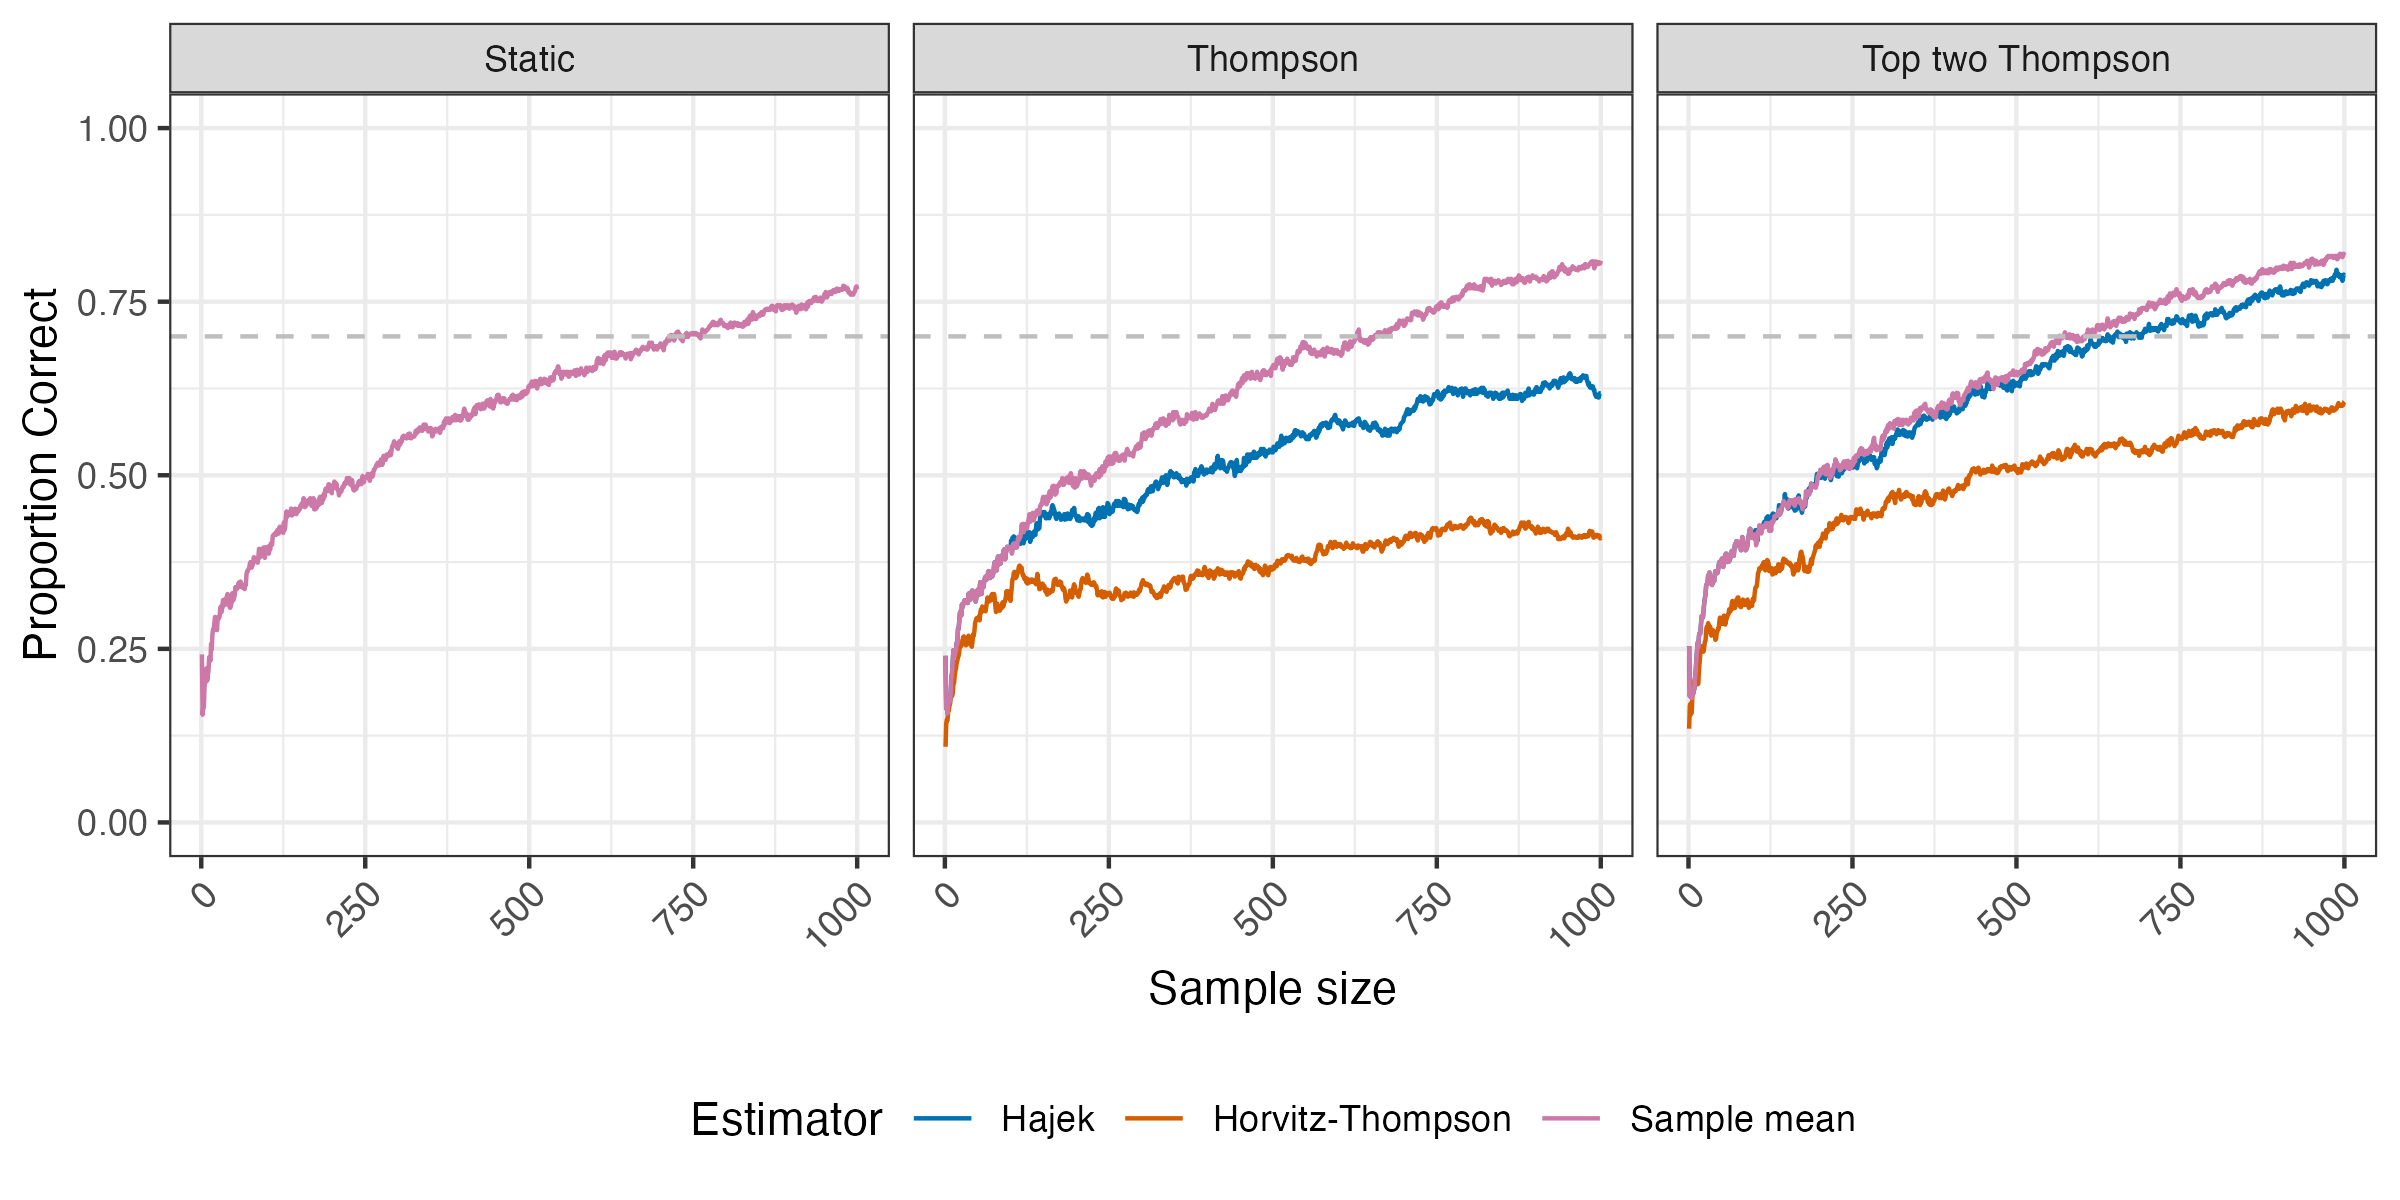
\includegraphics[width=\textwidth]{../assets/joint_correct4.png} 
\end{figure}

\end{frame}


%%%%%NOTE%%%%%
\note{
\scriptsize \singlespacing
Things to note:
\begin{wideitemize}
\item We trade off which arm we think is best
\end{wideitemize}
}

%-------------------------------------------------------------------------------%
\begin{frame}{Estimating procedures with TT Thompson}

\begin{figure}[htbp]
   \centering
   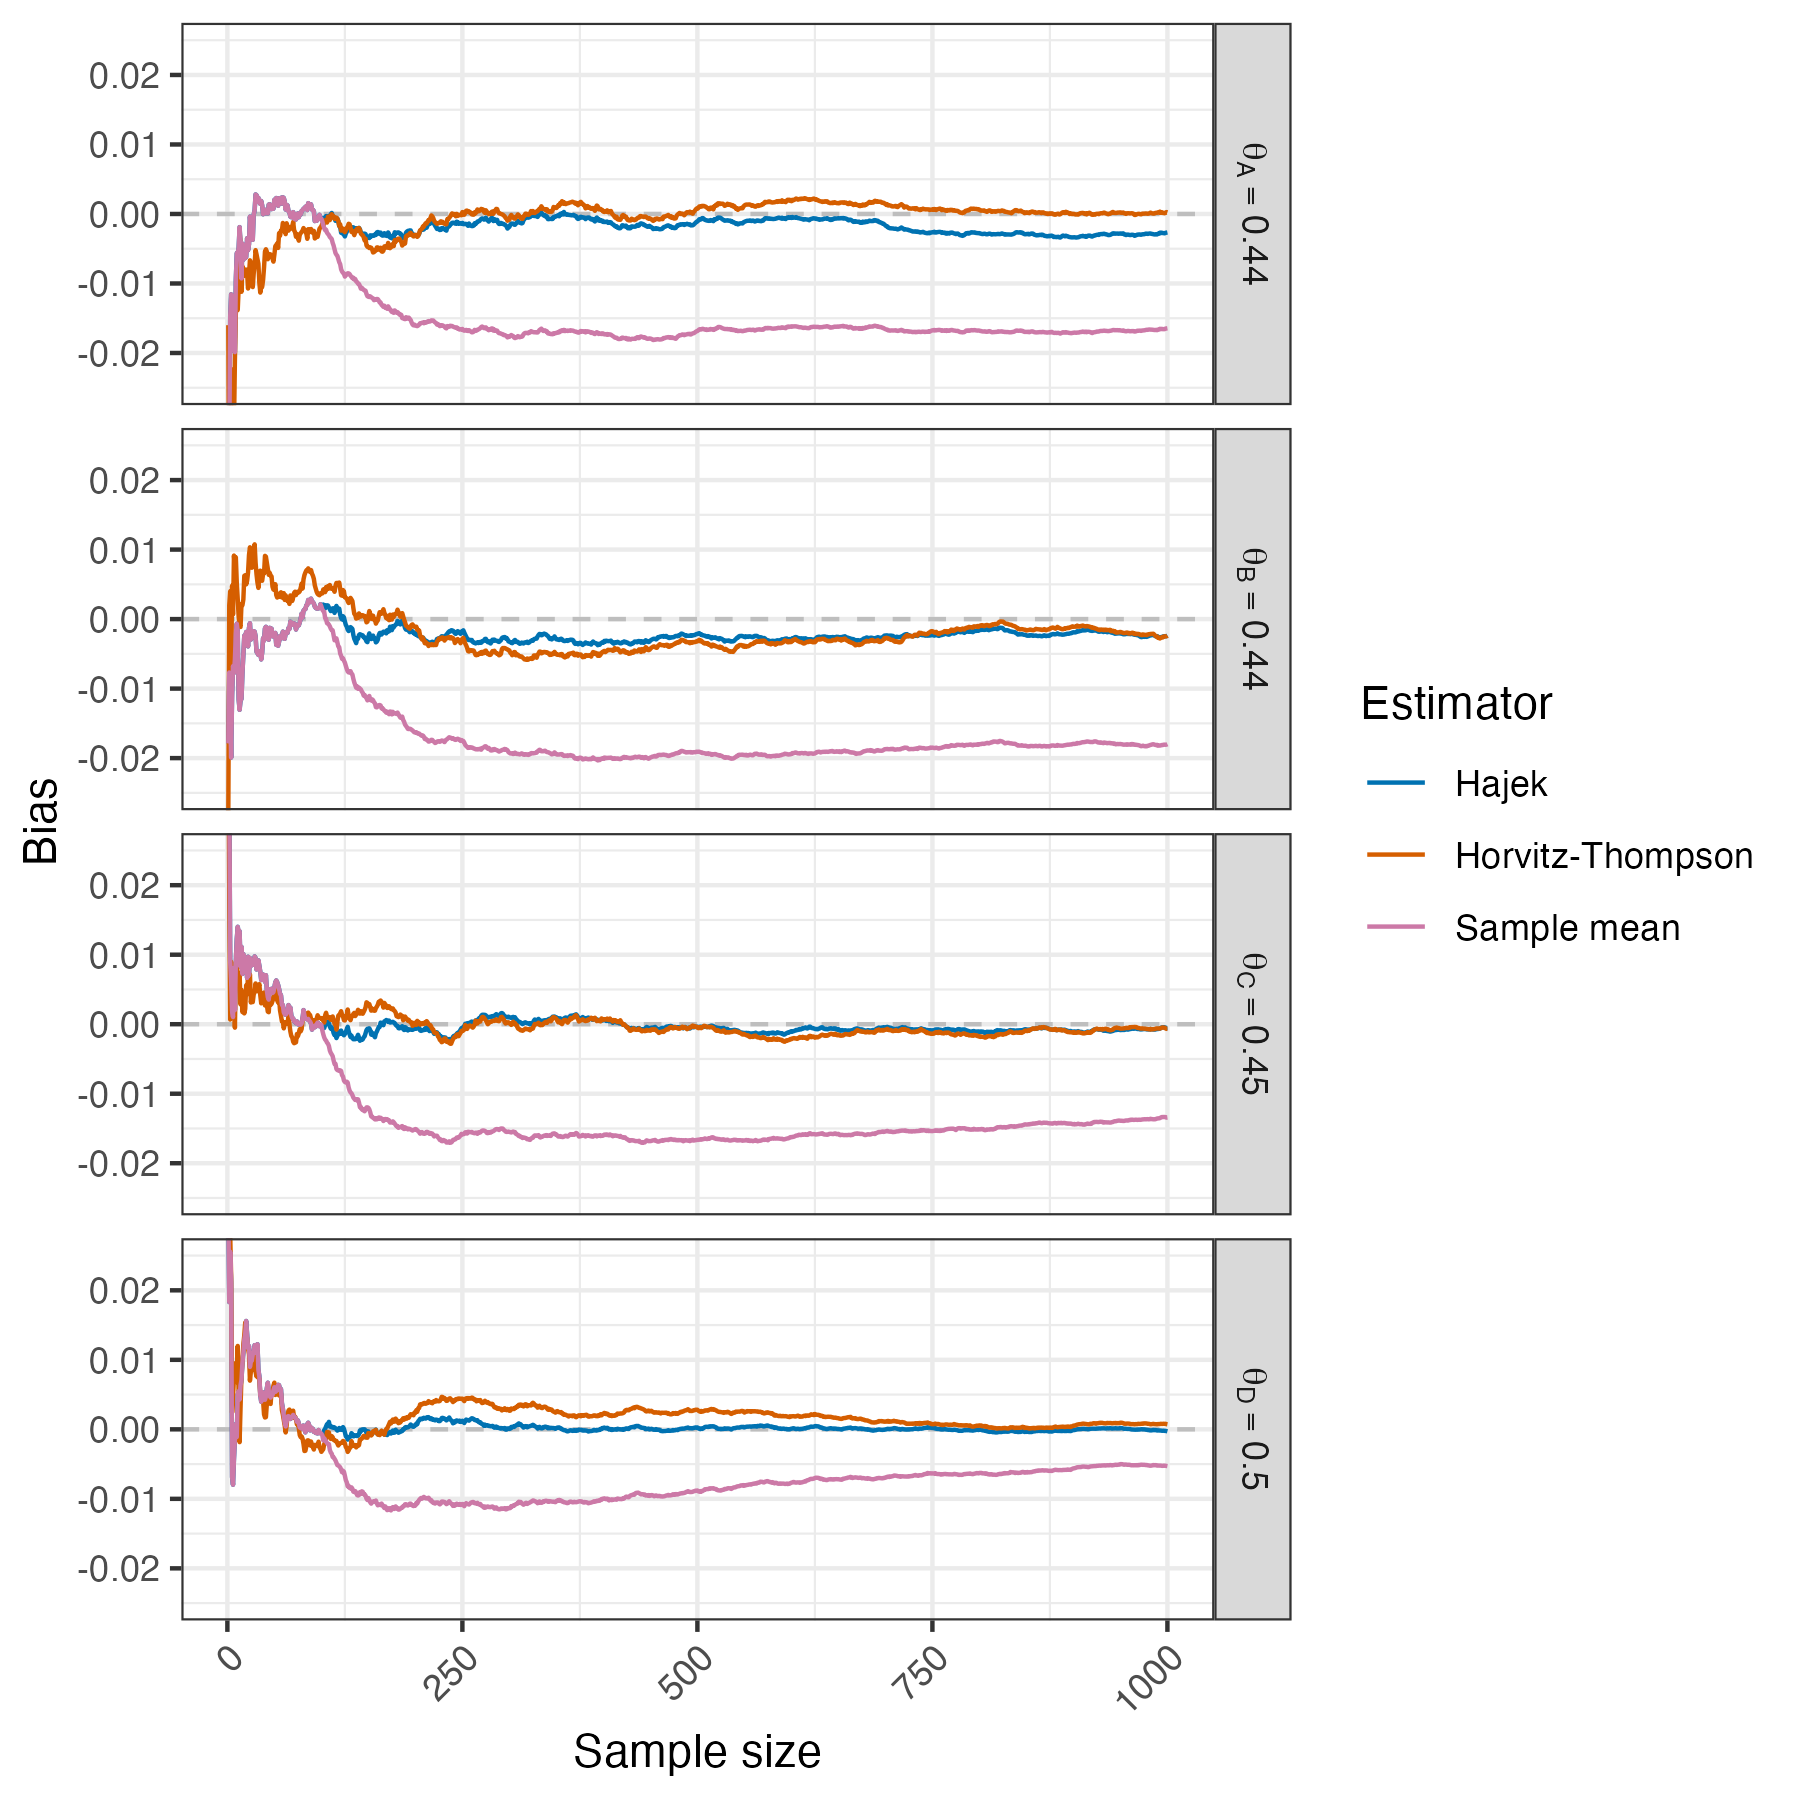
\includegraphics[width = 0.7\textwidth]{../assets/ttts_bias4.png} %
   \label{fig:example}
\end{figure}
\vskip -2 em
\hyperlink{debias}{\beamerbutton{Bias}}
\end{frame}


%%%%%NOTE%%%%%
\note{
\scriptsize \singlespacing

%\begin{wideitemize}
%\item xxx
%\end{wideitemize}
}

%-------------------------------------------------------------------------------%
\begin{frame}{Best arm identification}

\begin{wideitemize}
\item Why these types of designs work:\pause
\begin{itemize}
\item Strategic \textit{exploration} at the top end of the distribution\pause
%\item Cumulative-regret minimization algorithms are trading off exploration and exploitation\pause
\item Promising in the fixed-budget setting \citep{jourdan2022top} with good simulation-based results \citep{russo2016simple}\pause
\item Uniform random assignment will do well asymptotically \pause
\item But we can get closer to best policy faster in small, medium sized samples. 
\end{itemize}
\end{wideitemize}

\end{frame}


%%%%%NOTE%%%%%
\note{
\scriptsize \singlespacing

%\begin{wideitemize}
%\item xxx
%\end{wideitemize}
}
%-------------------------------------------------------------------------------%
\begin{frame}{A few more questions}

\begin{wideitemize}
%\item How long should we run the experiment?\pause
\item Do we care about frequentist inference ex-post?
\end{wideitemize}

\end{frame}


%%%%%NOTE%%%%%
\note{
\scriptsize \singlespacing

%\begin{wideitemize}
%\item xxx
%\end{wideitemize}
}
%-------------------------------------------------------------------------------%
\begin{frame}{Inference on data-driven quantities}


\begin{wideitemize}
\item Naive inference on ``best'' arm is positively biased \pause
\item[$\rightarrow$] version of winner's curse
\end{wideitemize}

\end{frame}


%%%%%NOTE%%%%%
\note{
\scriptsize \singlespacing

\begin{wideitemize}
\item xxxx
\end{wideitemize}
}

%-------------------------------------------------------------------------------%
\begin{frame}{Inference on data-driven quantities}

\begin{figure}[htbp] %  figure placement: here, top, bottom, or page
   \centering
   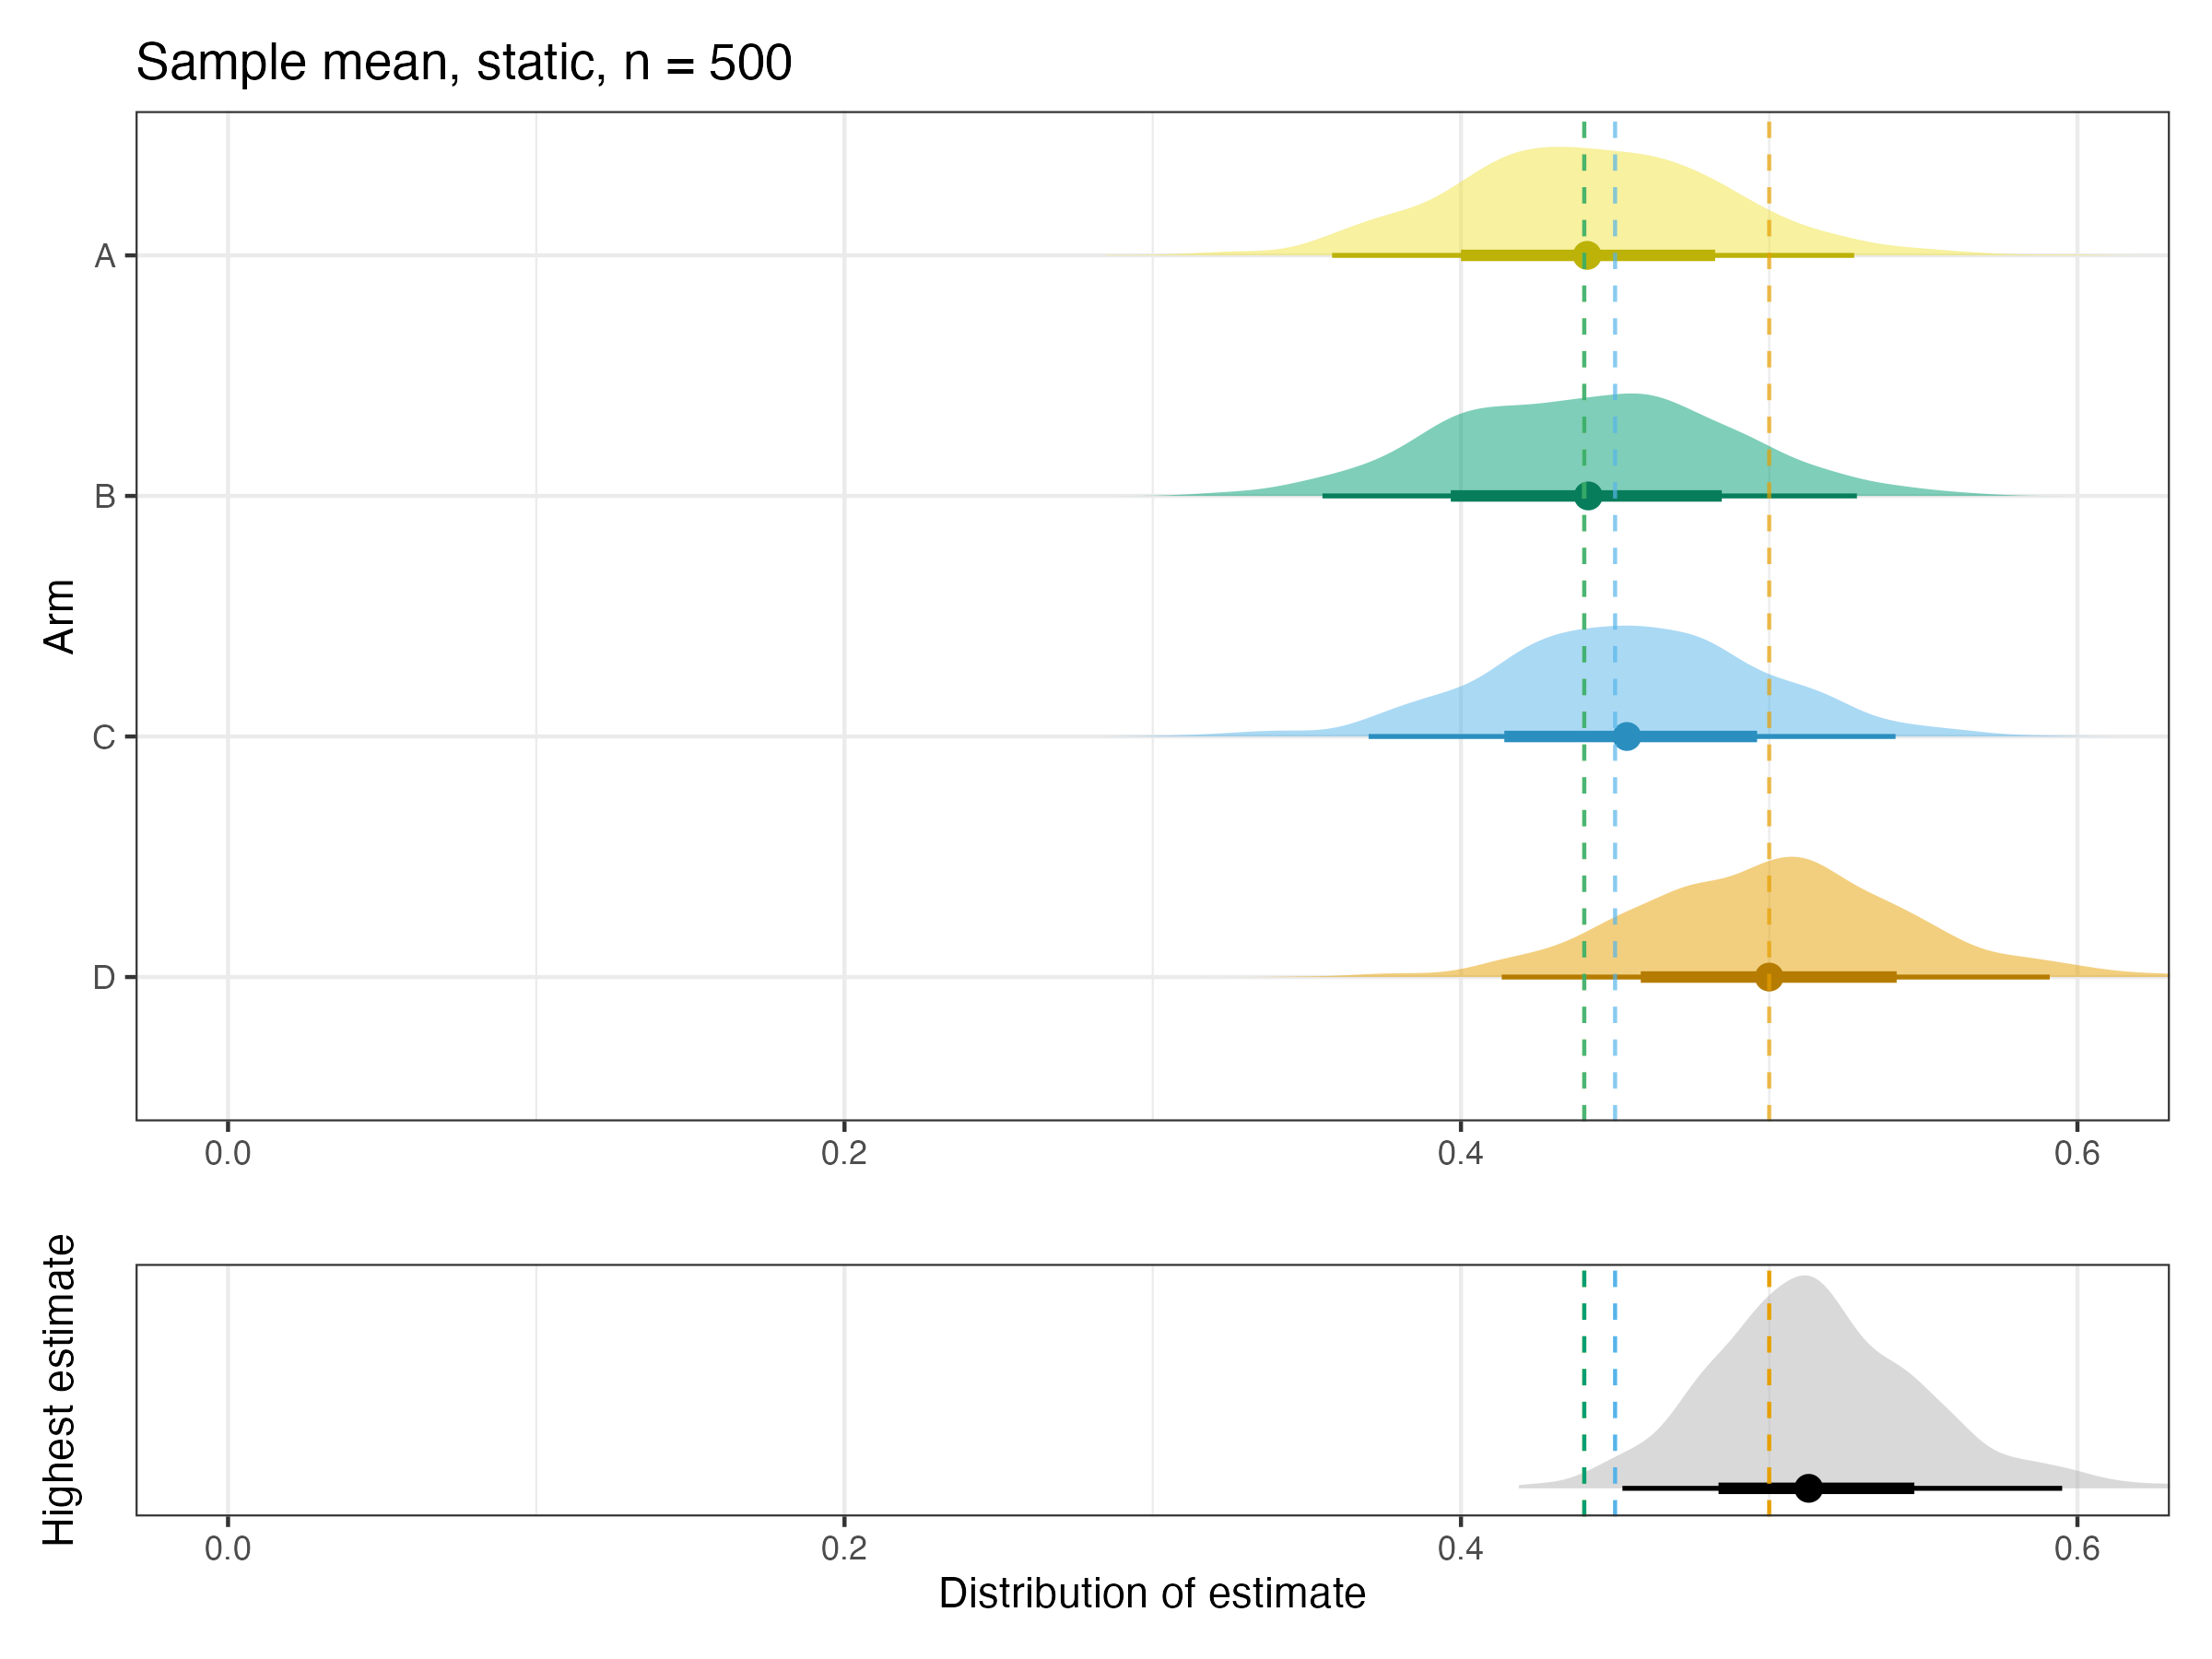
\includegraphics[width=\textwidth] {../assets/static_hjmax_500.png} 
\end{figure}

\end{frame}


%%%%%NOTE%%%%%
\note{
\scriptsize \singlespacing
Things to note:
\begin{wideitemize}
\item We trade off which arm we think is best
\end{wideitemize}
}

%-------------------------------------------------------------------------------%
\begin{frame}{Inference on data-driven quantities}

\begin{figure}[htbp] %  figure placement: here, top, bottom, or page
   \centering
   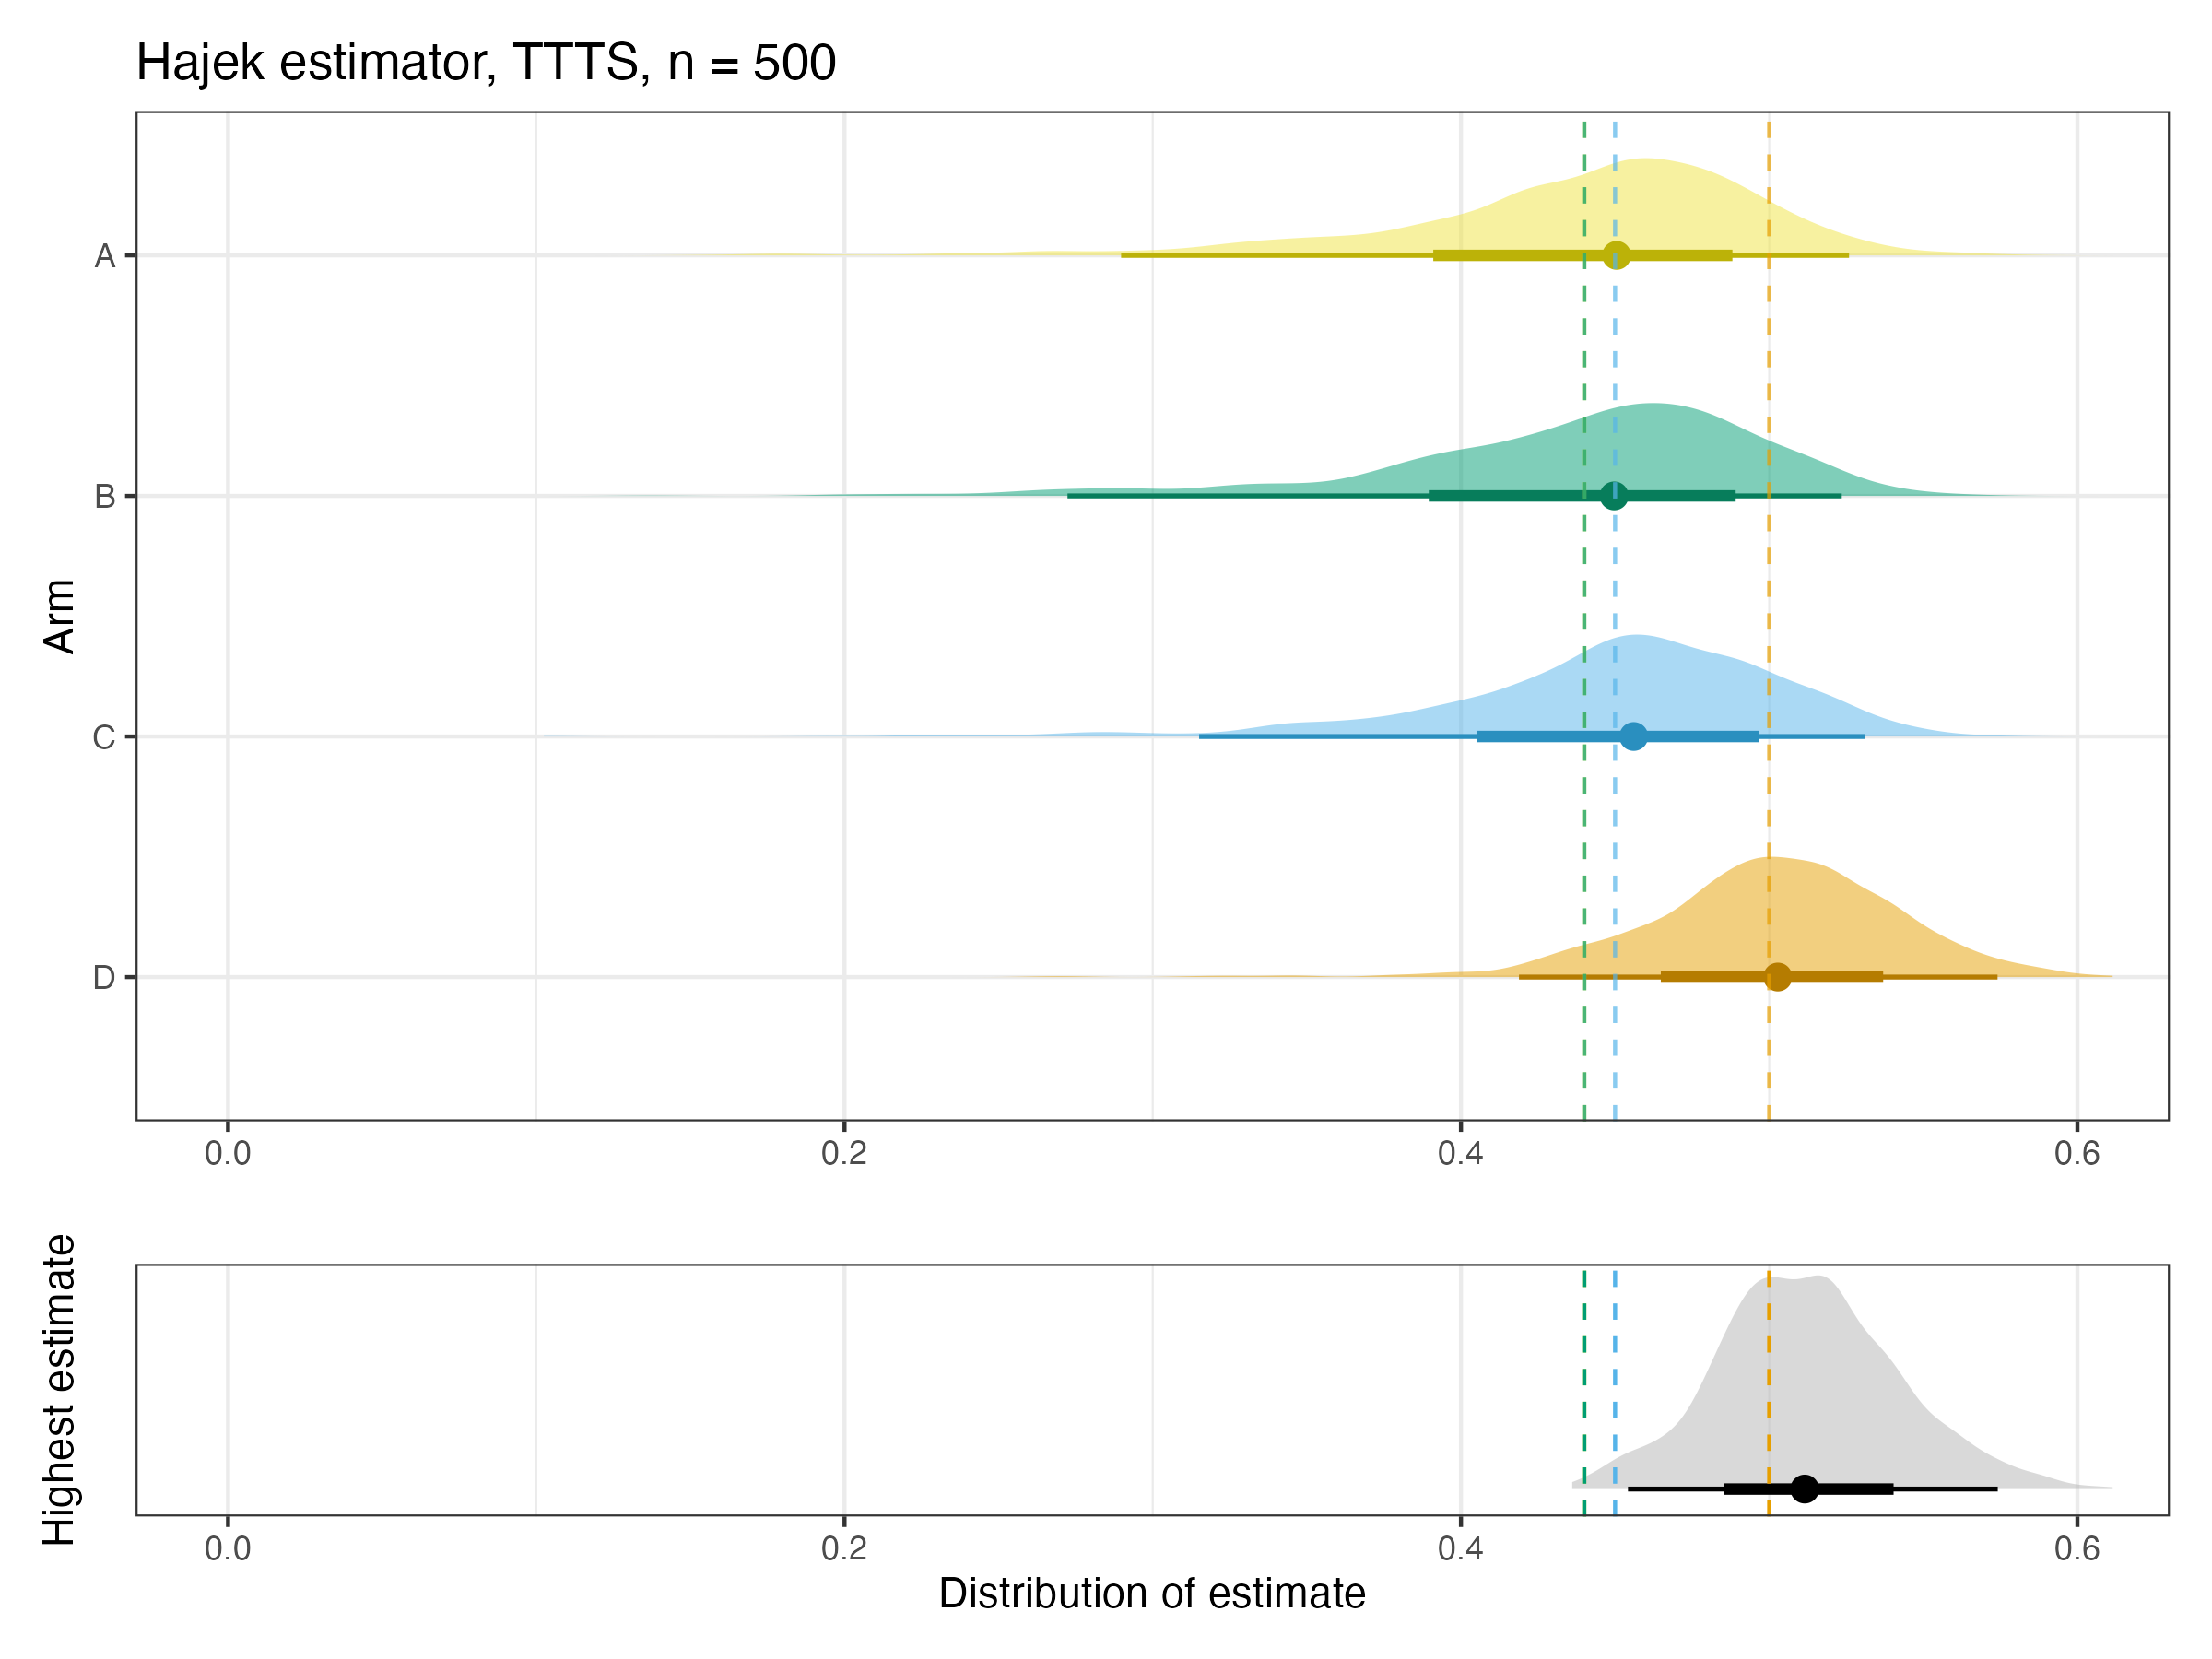
\includegraphics[width=\textwidth] {../assets/ttts_hjmax_500.png} 
\end{figure}

\end{frame}


%%%%%NOTE%%%%%
\note{
\scriptsize \singlespacing
Things to note:
\begin{wideitemize}
\item We trade off which arm we think is best
\end{wideitemize}
}

%-------------------------------------------------------------------------------%
\begin{frame}{Inference on data-driven quantities}


\begin{wideitemize}
\item[$\rightarrow$] Some tools for selective inference on non-adaptively collected data \citep{andrews2024inference}\pause
\item Or use cross-fitting \pause
\item For adaptively collected data, without further assumptions on experiment design, just conduct inference using last batch of data collected \citep{chen2023optimal}
\end{wideitemize}

\end{frame}


%%%%%NOTE%%%%%
\note{
\scriptsize \singlespacing

\begin{wideitemize}
\item xxxx
\end{wideitemize}
}

%-------------------------------------------------------------------------------%
\begin{frame}{Evaluation metric}

\begin{figure}[htbp] %  figure placement: here, top, bottom, or page
   \centering
   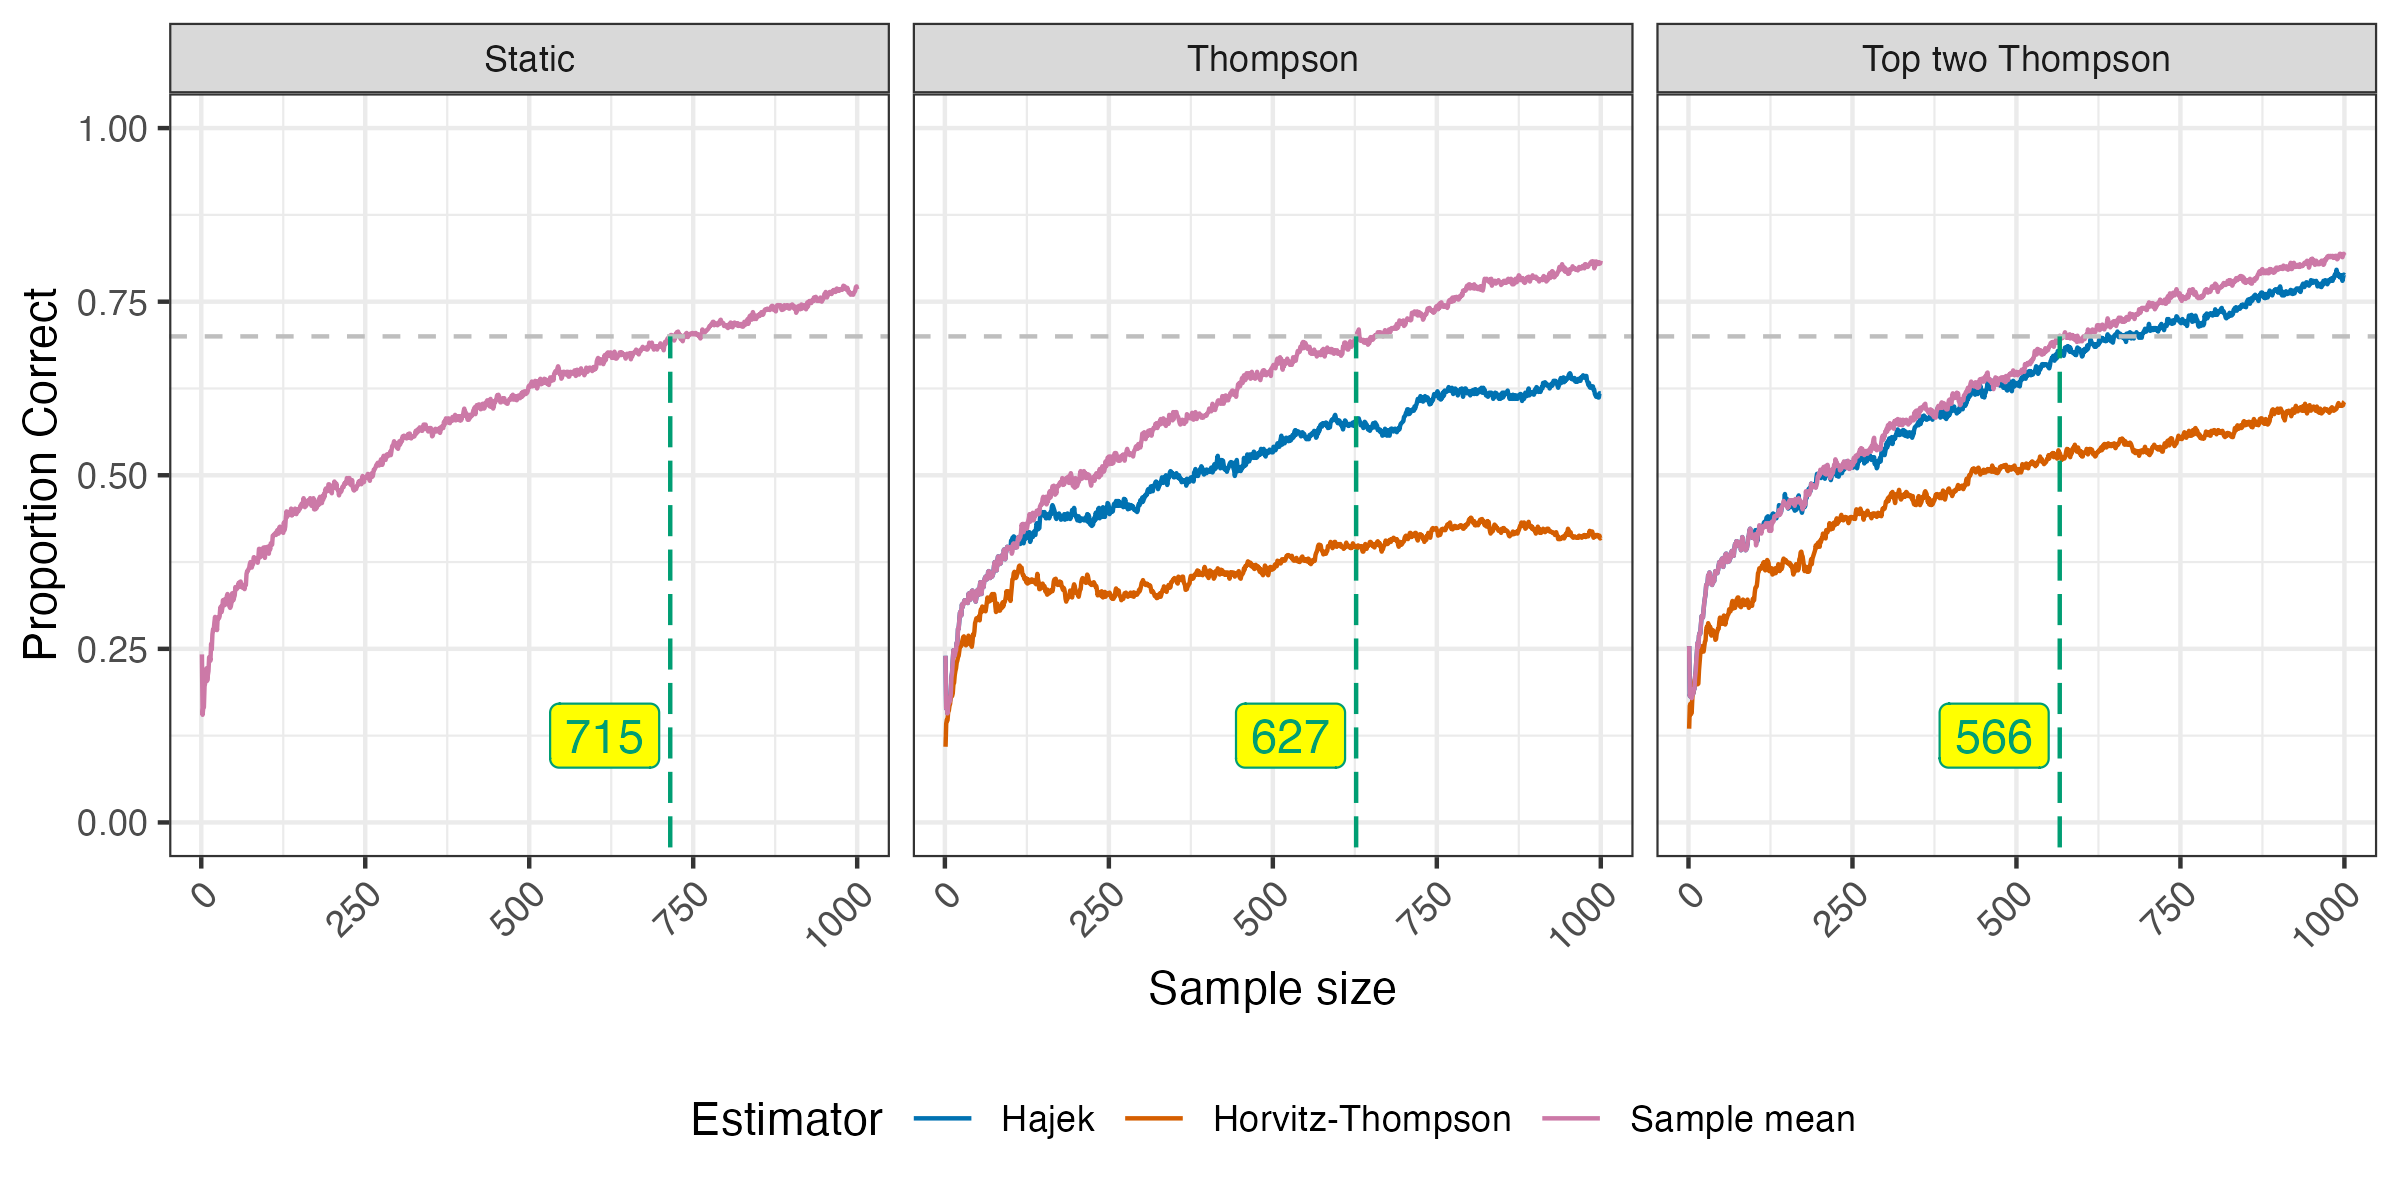
\includegraphics[width=\textwidth]{joint_correct4_lines.png} 
\end{figure}

\end{frame}


%%%%%NOTE%%%%%
\note{
\scriptsize \singlespacing
Things to note:
\begin{wideitemize}
\item We trade off which arm we think is best
\end{wideitemize}
}

%-------------------------------------------------------------------------------%
\begin{frame}{Confidence intervals with adaptively collected data}

Even for non data-driven hypotheses, with adaptively collected data, we get non-normality in distribution of estimators. 

\begin{figure}[htbp]
   \centering
   \includegraphics[width = 0.75\textwidth]{\figpath skewed_dist.png} %
   \label{fig:example}
\end{figure}

\cite{hadad2021confidence}\hfill
\end{frame}


%%%%%NOTE%%%%%
\note{
\scriptsize \singlespacing

%\begin{wideitemize}
%\item xxx
%\end{wideitemize}
}
%-------------------------------------------------------------------------------%
\begin{frame}{Inference on data-driven quantities}

\begin{figure}[htbp] %  figure placement: here, top, bottom, or page
   \centering
   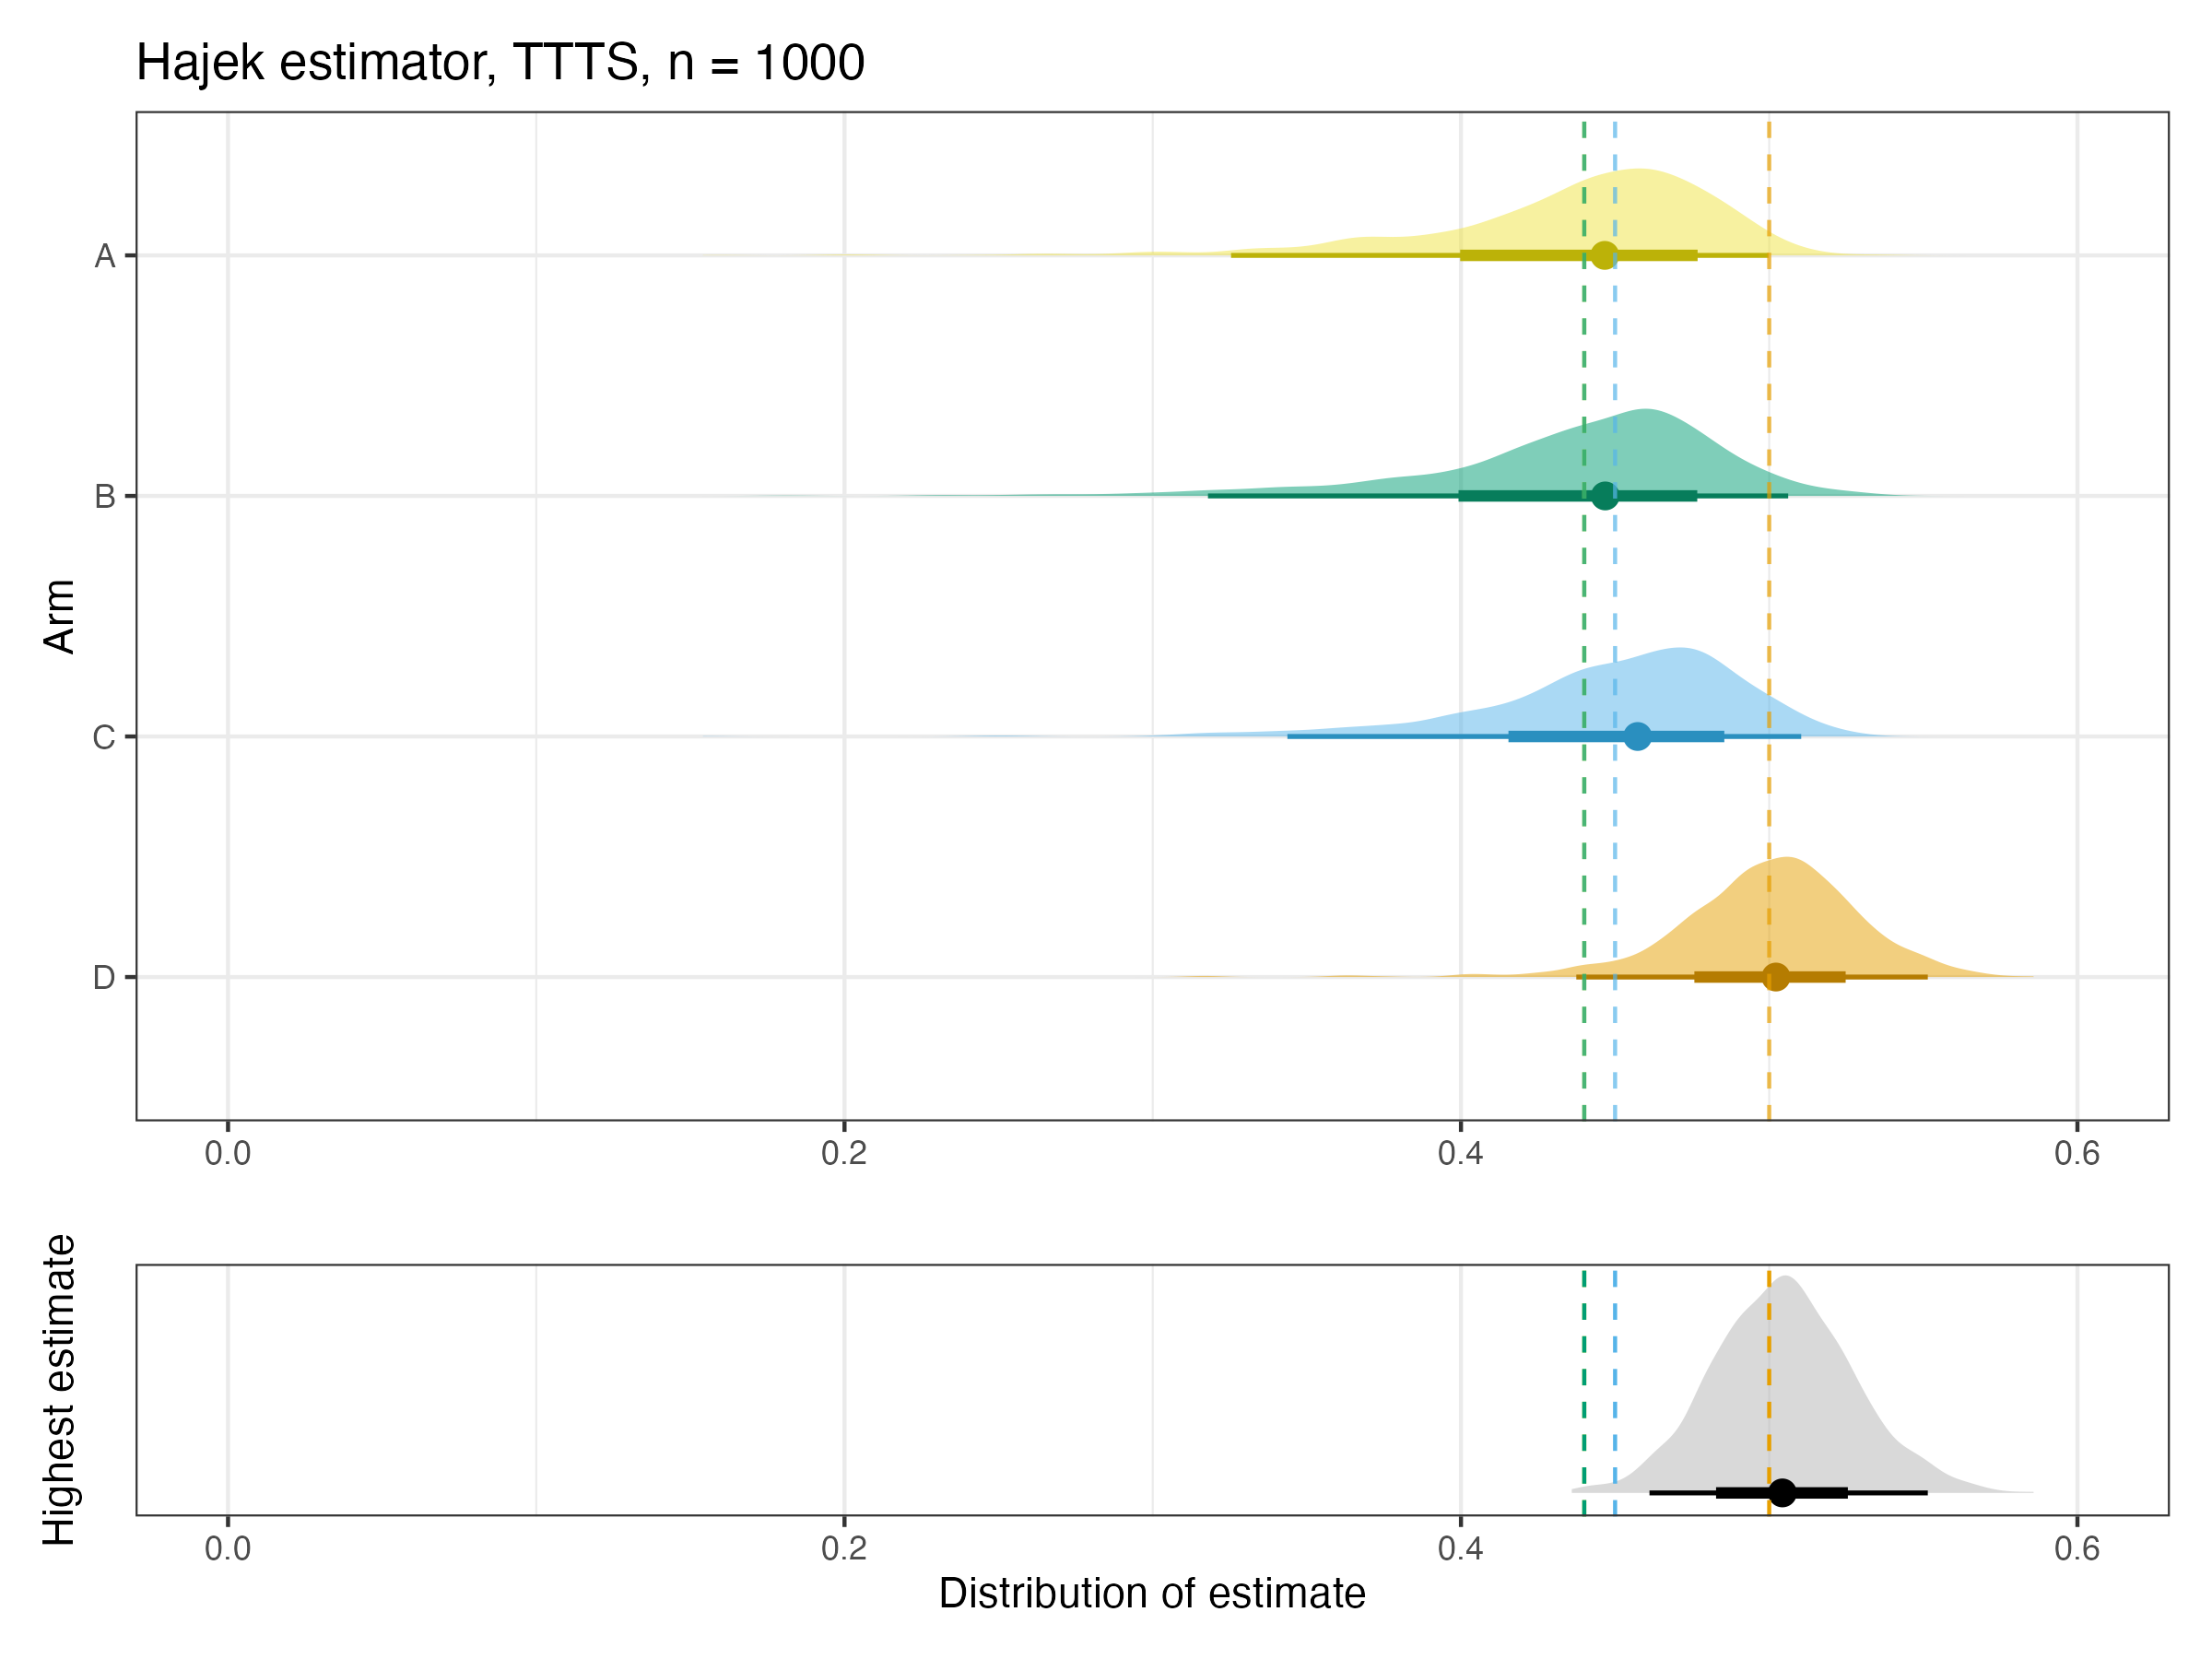
\includegraphics[width=\textwidth] {../assets/ttts_hjmax_1000.png} 
\end{figure}

\end{frame}


%%%%%NOTE%%%%%
\note{
\scriptsize \singlespacing
Things to note:
\begin{wideitemize}
\item We trade off which arm we think is best
\end{wideitemize}
}

%-------------------------------------------------------------------------------%

\begin{frame}{Confidence intervals with adaptively collected data}

Some solutions:
\begin{wideitemize}
\item \cite{hadad2021confidence}: adaptively re-weight the terms of the augmented inverse propensity weighting estimator, controlling for contributions of each term to estimator's variance.
\begin{wideitemize}
\item Requires that the propensity score decay at a slow enough rate.
\item Contextual setting: \cite{zhan2021off}\pause
\end{wideitemize}
\item \cite{deshpande2017accurate}: augment OLS estimator with $\W-$ ``decorrelation'' matrix to remove the effects of adaptivity. \pause
\item \cite{zhang2020inference}: batched OLS hypothesis testing; OLS estimates are asymptotically normal \textit{within} batches. Then combine batch-wise statistics and compare to simulated null distribution 
\begin{wideitemize}
\item Requires batched assignment. 
\end{wideitemize}
\end{wideitemize}


\end{frame}


%%%%%NOTE%%%%%
\note{
\scriptsize \singlespacing

\begin{wideitemize}
\item Hadad et al. (2019) propose an augmented version of the IPW estimator, which allows for an optional conditional means model with evaluation weights that, under specified conditions, achieves asymptotic normality for adaptively weighted estimates even in the no-signal setting. When there is a unique best arm, however, these necessary conditions for asymptotic normality of IPW-type estimators may hold in the absence of evaluation weights. 
\item Deshpande et al. (2020) propose a W-decorrelation estimator, under which they augment the standard OLS estimate with a decorrelation matrix. This matrix is a function of a tuned regularization parameter, which trades off bias and variance. 
\item Zhang et al. (2020) propose a ``batched'' OLS hypothesis testing procedure, noting the asymptotic normality of OLS estimates within batches. They construct a test statistic by combining batch-wise t-statistics and compare it to a simulated null distribution in order to obtain a p-value. The authors demonstrate that this testing procedure has reliable Type-1 error control in small samples and is robust to non-stationarity.
\item See also Raaz Dwivedi's presentation earlier in this workshop (with Susan Murphy?)
\end{wideitemize}
}
%-------------------------------------------------------------------------------%
\begin{frame}{Confidence intervals with adaptively collected data}



\begin{wideitemize}
\item You still need an appropriate design (sufficient probability floors, batch-wise assignment) for these methods to work. 
\end{wideitemize}

\end{frame}


%%%%%NOTE%%%%%
\note{
\scriptsize \singlespacing

%\begin{wideitemize}
%\item xxx
%\end{wideitemize}
}
%-------------------------------------------------------------------------------%
\begin{frame}{Confidence intervals with adaptively collected data}

\begin{center}
\begin{tikzpicture}
\node(a){
\footnotesize
    \begin{tblr}{
    colspec={M{1.2cm}M{1cm}M{6cm}},row{2-5}={7ex},
      cells={halign=c, valign = m},
      stretch = 3
      }
      \SetCell[c=2]{} Advertisements &&  {Estimated \\ mean response}  \\
	 \includegraphics[width = 1cm]{\figpath tv-ad.png} & \textbf A & \SetCell[r=5]{c} \vspace*{-6em} 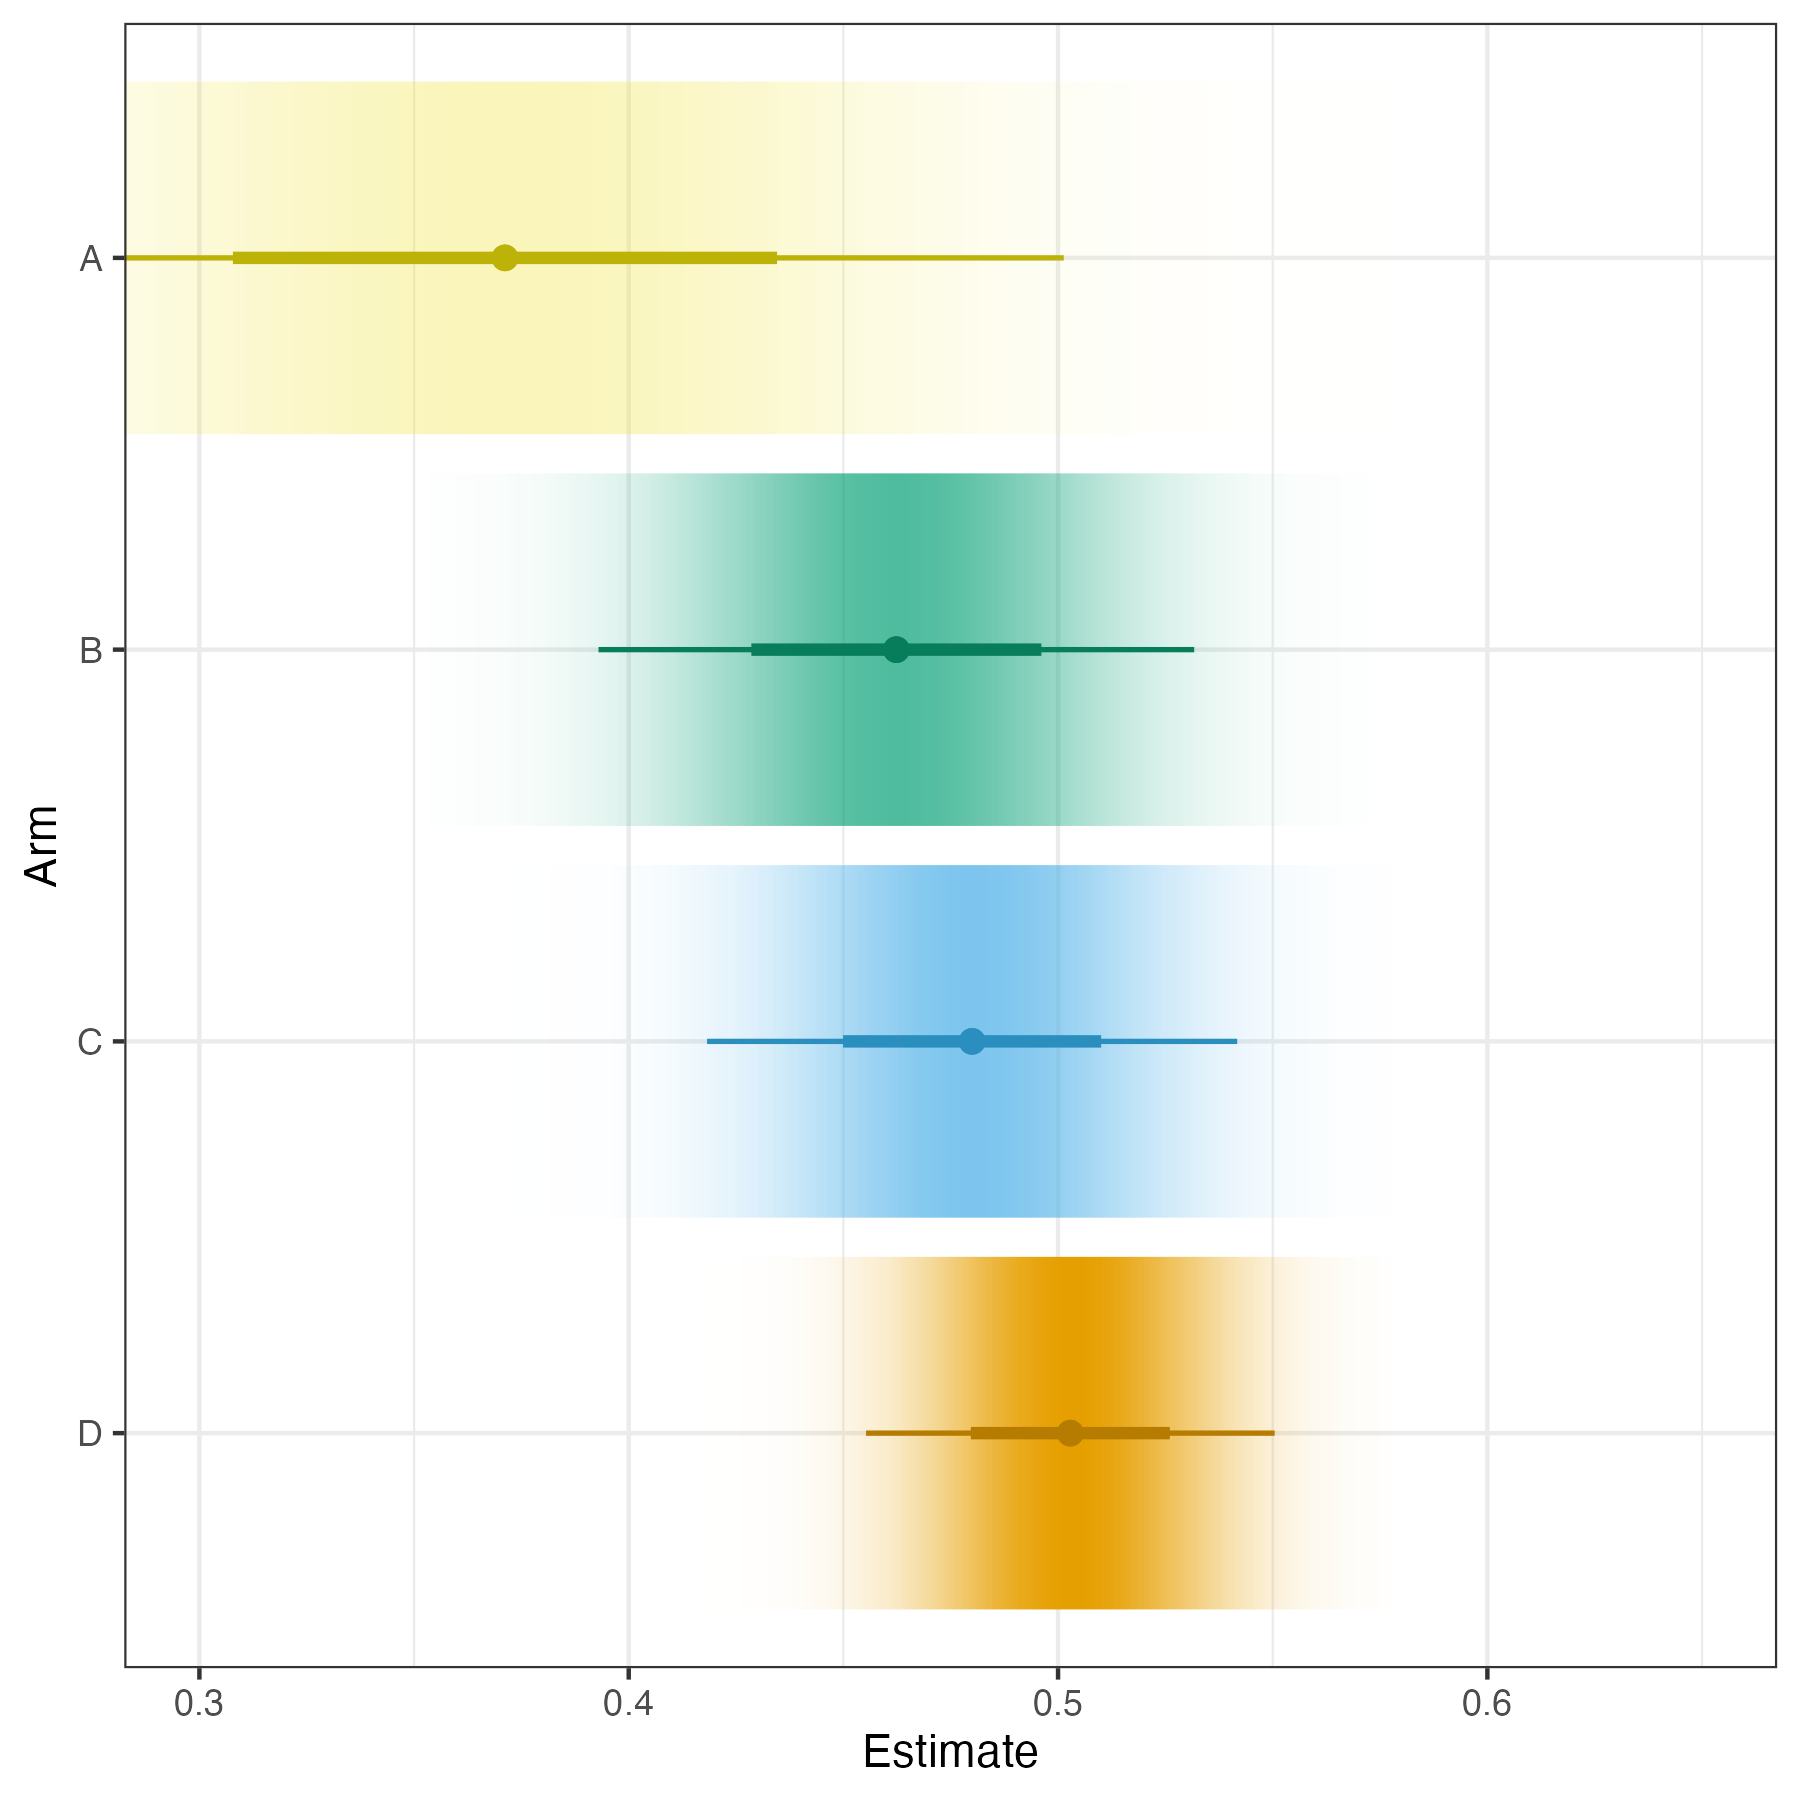
\includegraphics[width = 0.52\textwidth] {../assets/ttts_estimate4.png} \\
	\includegraphics[width = 1cm]{\figpath tv-ad.png} & \textbf B &\\
	\includegraphics[width = 1cm]{\figpath tv-ad.png} & \textbf C &\\
	\includegraphics[width = 1cm]{\figpath tv-ad.png} & \textbf D &\\ \vspace*{-30em} \ \\
    \end{tblr}
 };
%\onslide<2>{\node at(a.center)[draw, red,line width=3pt,ellipse, minimum width=80pt, minimum height=50pt,rotate=0pt,yshift=-60pt, xshift = 80pt]{};}
\end{tikzpicture}   
\end{center}

\end{frame}



%%%%%NOTE%%%%%
\note{
\scriptsize \singlespacing

%\begin{wideitemize}
%\item xxx
%\end{wideitemize}

}
%-------------------------------------------------------------------------------%
\begin{frame}{Confidence intervals with adaptively collected data}

\begin{center}
\begin{tikzpicture}
\node(a){
\footnotesize
    \begin{tblr}{
    colspec={M{1.2cm}M{1cm}M{6cm}},row{2-5}={7ex},
      cells={halign=c, valign = m},
      stretch = 3
      }
      \SetCell[c=2]{} Advertisements &&  {Adjusted estimated \\ mean response}  \\
	 \includegraphics[width = 1cm]{\figpath tv-ad.png} & \textbf A & \SetCell[r=5]{c} \vspace*{-6em} 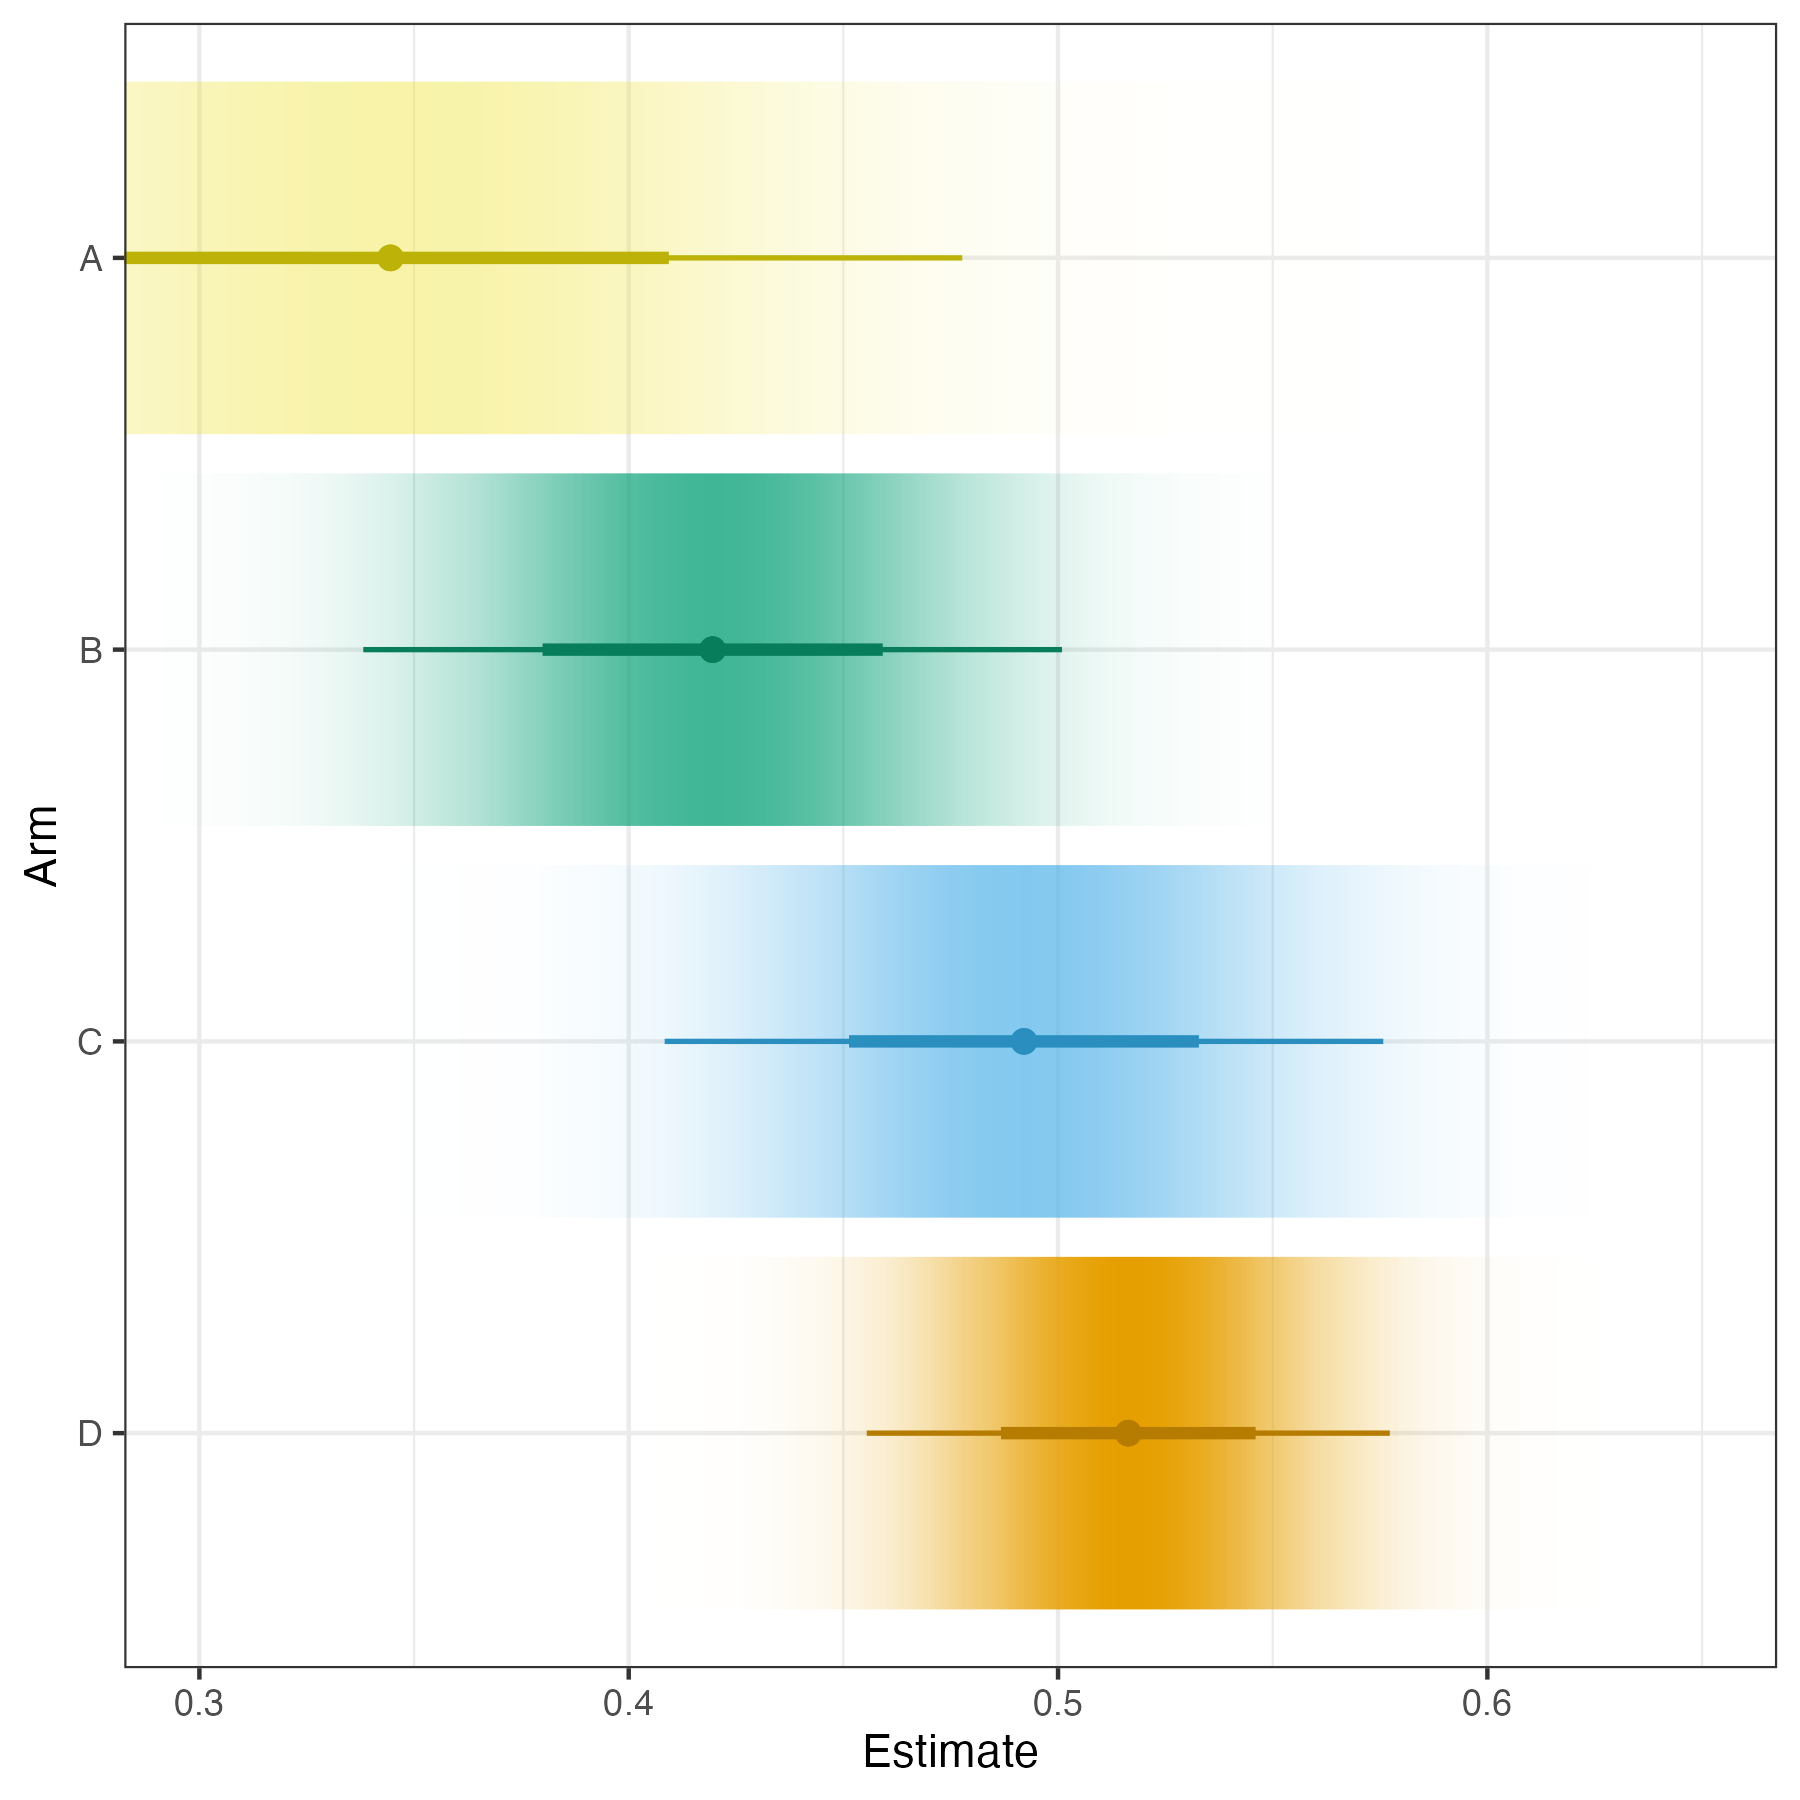
\includegraphics[width = 0.52\textwidth] {../assets/ttts_estimate_adjusted4.png} \\
	\includegraphics[width = 1cm]{\figpath tv-ad.png} & \textbf B &\\
	\includegraphics[width = 1cm]{\figpath tv-ad.png} & \textbf C &\\
	\includegraphics[width = 1cm]{\figpath tv-ad.png} & \textbf D &\\ \vspace*{-30em} \ \\
    \end{tblr}
 };
%\onslide<2>{\node at(a.center)[draw, red,line width=3pt,ellipse, minimum width=80pt, minimum height=50pt,rotate=0pt,yshift=-60pt, xshift = 80pt]{};}
\end{tikzpicture}   
\end{center}

\end{frame}



%%%%%NOTE%%%%%
\note{
\scriptsize \singlespacing

%\begin{wideitemize}
%\item xxx
%\end{wideitemize}

}
%-------------------------------------------------------------------------------%
\begin{frame}[c]{Confidence intervals with adaptively collected data}
\centering
\texttt{banditsCI} package

\end{frame}


%%%%%NOTE%%%%%
\note{
\scriptsize \singlespacing

%\begin{wideitemize}
%\item xxx
%\end{wideitemize}
}
%-------------------------------------------------------------------------------%
\begin{frame}[c]

\Large

\centering
\textcolor{Maroon}{Should the campaign buy ads at all?}

\end{frame}


%%%%%NOTE%%%%%
\note{
\scriptsize \singlespacing

%\begin{wideitemize}
%\item xxx
%\end{wideitemize}
}
%-------------------------------------------------------------------------------%
\begin{frame}{Why we experiment}

\begin{figure}[htbp]
   \includegraphics[width = \textwidth]{\figpath biden_ads_yesno.png}
   \label{fig:bidenads}
\end{figure}

\end{frame}


%%%%%NOTE%%%%%
\note{
\scriptsize \singlespacing

%\begin{wideitemize}
%\item xxx
%\end{wideitemize}
}
%-------------------------------------------------------------------------------%
\begin{frame}[c]{Why we experiment}

Suppose approval rating is at 45\%\pause; can we improve over this with \textit{any} advertising strategy?\pause

\ \\

For an assignment policy $\pi \in \Pi$\pause


\begin{equation*}
\pi^* = \argmax_{\pi \in \Pi} \E[\langle \Y_i,\pi(\X_i) \rangle]
\label{eq:policy}
\end{equation*}
\pause

\begin{align*}
\textrm{H}_0 :  & \E\left[\langle \Y_i,\pi(\X_i) \rangle\right] = 0.45 \ \ \forall \pi \in \Pi \\  
\textrm{H}_A:  & \exists \ \pi \in \Pi:  \E\left[\langle \Y_i,\pi(\X_i) \rangle\right] > 0.45 \\
\end{align*}

\end{frame}


%%%%%NOTE%%%%%
\note{
\scriptsize \singlespacing

%\begin{wideitemize}
%\item xxx
%\end{wideitemize}
}
%-------------------------------------------------------------------------------%
\begin{frame}[c]{Why we experiment}

For uniform policies: 

\begin{align*}
\textrm{H}_0 :  \theta_{w} = 0.45 \ \ \forall w \in \ww \\  
\textrm{H}_A: \exists \ w \in \ww:  \theta_{w} > 0.45 \\
\end{align*}

\end{frame}


%%%%%NOTE%%%%%
\note{
\scriptsize \singlespacing

%\begin{wideitemize}
%\item xxx
%\end{wideitemize}
}
%-------------------------------------------------------------------------------%
\begin{frame}[c]{Why we experiment}

\begin{wideitemize}
\item It doesn't make sense to test this with pooled data in the static setting if some of the advertisements are worse than status quo\pause
\begin{itemize}
\item[$\rightarrow$] Instead: test each message, implement  adjustments for multiple testing procedures. \pause
\end{itemize}
\item For algorithms that minimize \textcolor{Contrast1}{cumulative regret}, assignment will move towards optimal allocation, and we can test directly whether experimental allocation is better than status quo. 
\end{wideitemize}

\end{frame}


%%%%%NOTE%%%%%
\note{
\scriptsize \singlespacing

%\begin{wideitemize}
%\item xxx
%\end{wideitemize}
}
%-------------------------------------------------------------------------------%
\begin{frame}{Cumulative regret}
\begin{equation*}
R_{cumulative}(\tilde\pi)  = \sum_{i = 1}^n \left(\E\left[\langle \Y_i,\pi^* \rangle\right] - \E\left[\langle \Y_i,\tilde \pi(\HB_i) \rangle\right] \right)
\label{eq:regret}
\end{equation*}

\end{frame}


%%%%%NOTE%%%%%
\note{
\scriptsize \singlespacing

%\begin{wideitemize}
%\item xxx
%\end{wideitemize}
}
%-------------------------------------------------------------------------------%
\begin{frame}{Inference on data-driven quantities}

\begin{figure}[htbp] %  figure placement: here, top, bottom, or page
   \centering
   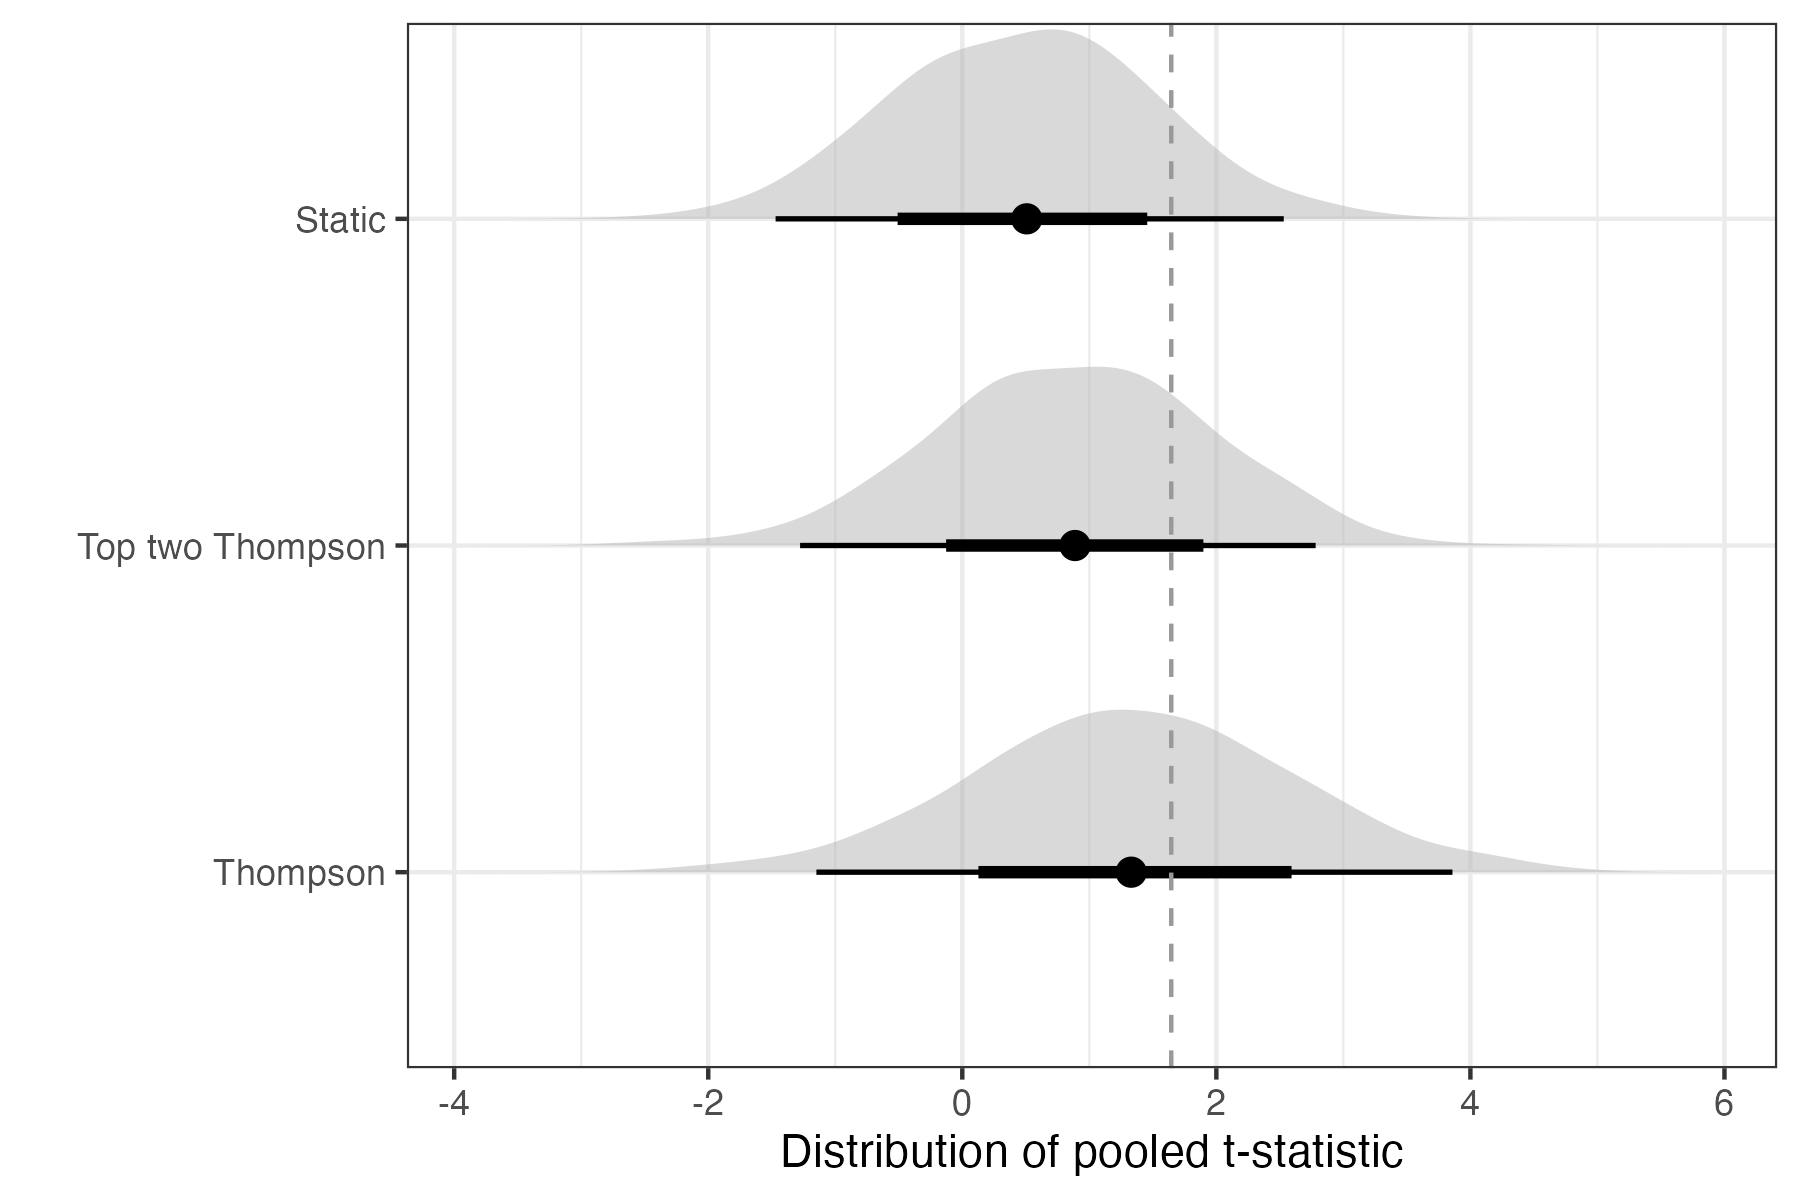
\includegraphics[width=\textwidth]{cum_benefit_joint.png} 
\end{figure}

\end{frame}


%%%%%NOTE%%%%%
\note{
\scriptsize \singlespacing

%\begin{wideitemize}
%\item xxx
%\end{wideitemize}
}

%-------------------------------------------------------------------------------%
\begin{frame}{Inference on data-driven quantities}

\begin{figure}[htbp] %  figure placement: here, top, bottom, or page
   \centering
   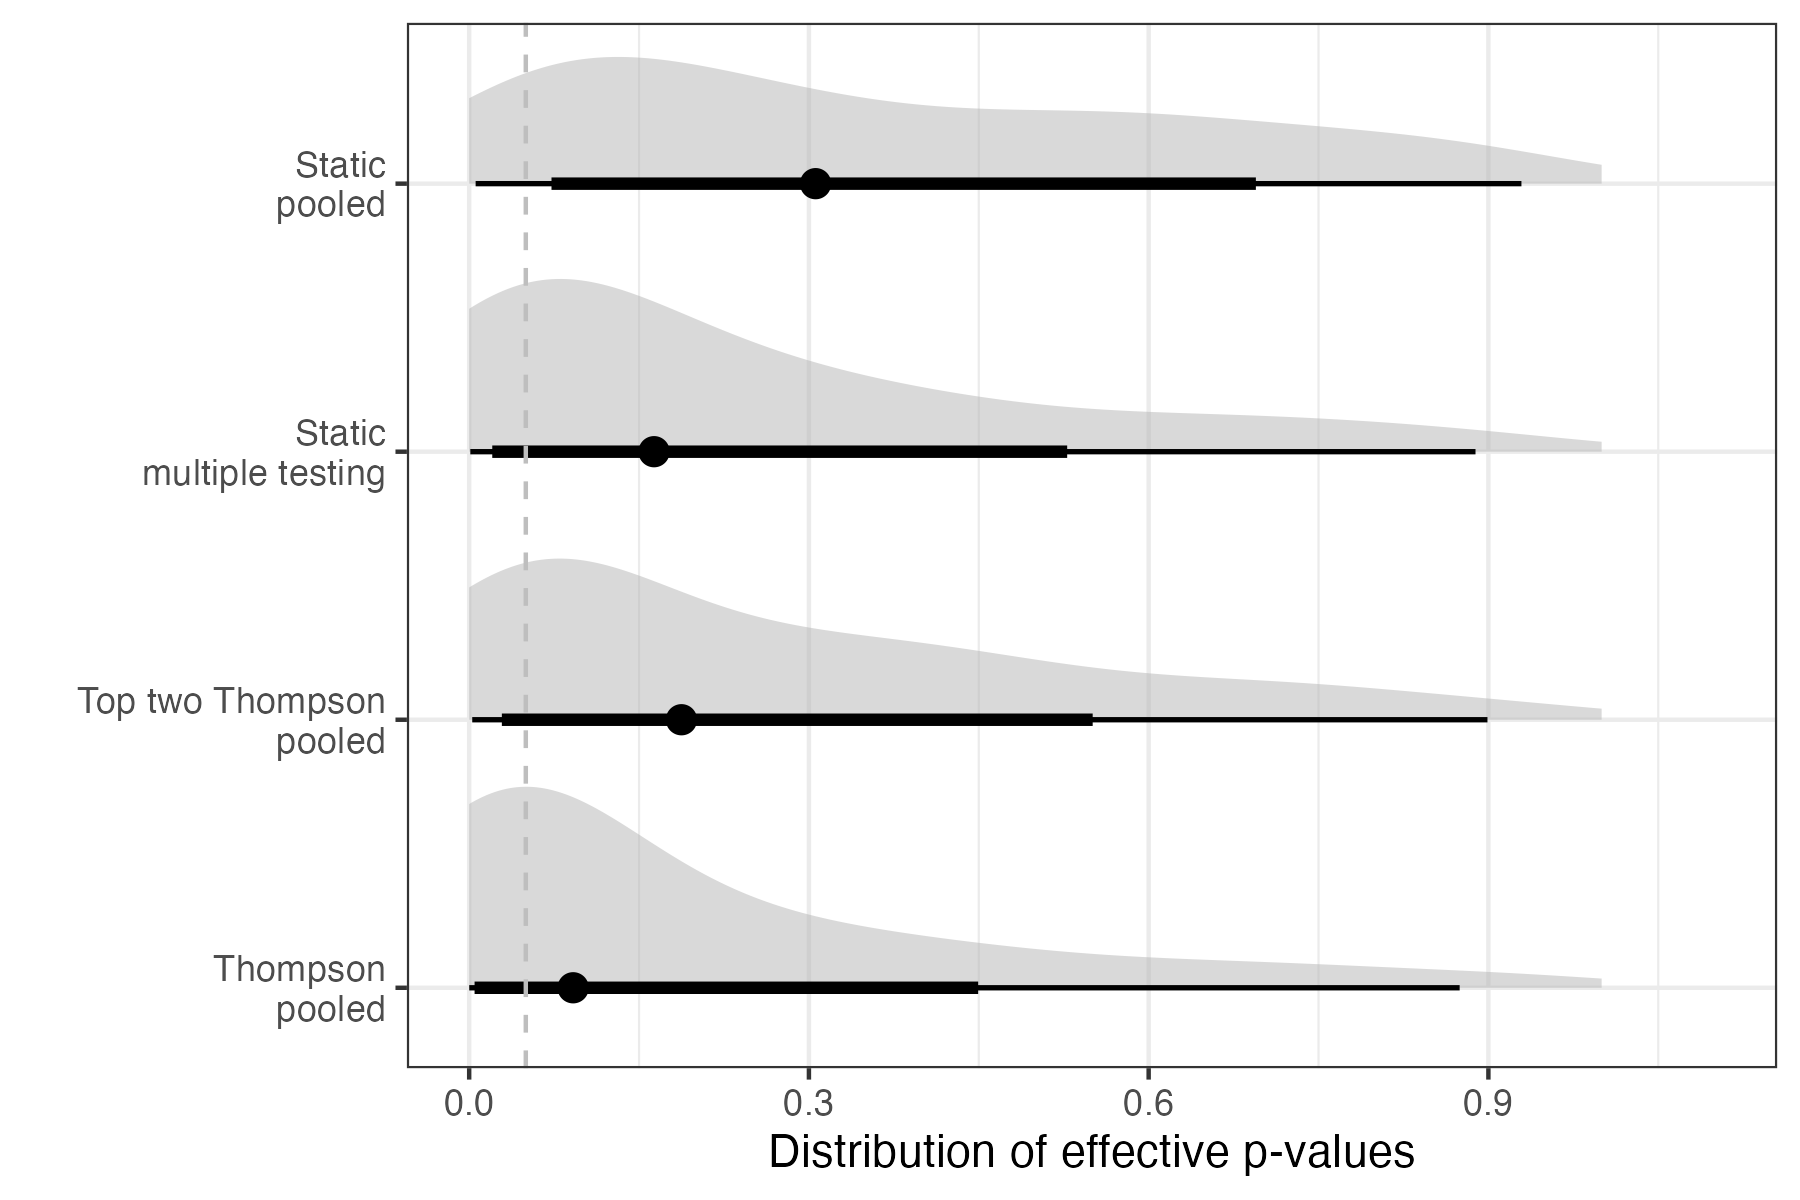
\includegraphics[width=\textwidth]{cum_benefit_joint_pval.png} 
\end{figure}

\end{frame}


%%%%%NOTE%%%%%
\note{
\scriptsize \singlespacing

%\begin{wideitemize}
%\item xxx
%\end{wideitemize}
}

%-------------------------------------------------------------------------------%
\begin{frame}{Targeted subgroups}

\begin{figure}[htbp]
   \includegraphics[width = \textwidth]{\figpath biden_ads_groups.png}
   \label{fig:bidenads}
\end{figure}

\end{frame}


%%%%%NOTE%%%%%
\note{
\scriptsize \singlespacing

%\begin{wideitemize}
%\item xxx
%\end{wideitemize}
}
%-------------------------------------------------------------------------------%
\begin{frame}[c]

\Large

\centering
\textcolor{Maroon}{Which ads should the campaign run--for targeted groups?}

\end{frame}


%%%%%NOTE%%%%%
\note{
\scriptsize \singlespacing

%\begin{wideitemize}
%\item xxx
%\end{wideitemize}
}
%-------------------------------------------------------------------------------%
\begin{frame}{Bridging non-contextual and contextual settings}

\begin{wideitemize}
\item We want to allow that different treatments are best for different types of people. \pause
\item Assume known, non-overlapping covariate regions. \pause
\item Assume no information is shared across regions.
\end{wideitemize}

\end{frame}


%%%%%NOTE%%%%%
\note{
\scriptsize \singlespacing

%\begin{wideitemize}
%\item xxx
%\end{wideitemize}
}
%-------------------------------------------------------------------------------%
\begin{frame}[label = policy1]{Adaptive assignment}

{
      \centering
      \includegraphics[width=\textwidth]{ \figpath joint_concerns_figure-1.png}
      }
\vskip -2 em
\hyperlink{vcf}{\beamerbutton{Application I: Vaccine hesitancy}}
\end{frame}


%%%%%NOTE%%%%%
\note{
\scriptsize \singlespacing

%\begin{wideitemize}
%\item xxx
%\end{wideitemize}
}
%-------------------------------------------------------------------------------%
\begin{transitionframe}

  \begin{center}
    { \Large \textcolor{white}{Extending to the fully contextual setting}}
  \end{center}
  
\end{transitionframe}

%-------------------------------------------------------------------------------%}
\begin{frame}{Fully contextual setting}

\begin{wideitemize}
\item We're learning both contexts \textit{and} best context-specific treatments simultaneously. 
\end{wideitemize}

\end{frame}


%%%%%NOTE%%%%%
\note{
\scriptsize \singlespacing

%\begin{wideitemize}
%\item xxx
%\end{wideitemize}
}
%-------------------------------------------------------------------------------%
\begin{frame}{Planner's goal}
\onslide<1->
\begin{equation*}
\pi^* = \argmax_{\pi \in \Pi} \E[\langle \Y_i,\pi(\X_i) \rangle]
\label{eq:policy}
\end{equation*}
\pause


\begin{wideitemize}
\item\onslide<2-> Contextual \textbf{policy learning} \citep{kitagawa2018should,athey2021policy}
\item\onslide<3-> In practice, $\pi^*$ is unknowable
\item\onslide<4-> Proximate objective: run an experiment, and \textit{at the end of the experiment}, learn some policy $\hat \pi$ to minimize \textbf{simple regret} %\onslide<6->{ (note: fixed budget setting)}
\end{wideitemize}
%
%\onslide<5->{
%\begin{equation*}
%R_{simple}(\hat\pi)  = \E\left[\langle \Y_i,\pi^*(\X_i) \rangle\right] -\E\left[ \langle \Y_i,\hat \pi(\X_i) \rangle\right]
%\label{eq:regret}
%\end{equation*}
%}


\end{frame}


%%%%%NOTE%%%%%
\note{
\scriptsize \singlespacing

%\begin{wideitemize}
%\item xxx
%\end{wideitemize}
}
%-------------------------------------------------------------------------------%
\begin{frame}[label = policy2]

\scalebox{0.55}{\begin{minipage}{1.8\textwidth}
\begin{algorithm}[H]
%\tiny
    \caption{Batch-wise balanced linear Thompson sampling}
    \label{algg:bblts}
    \begin{algorithmic}[1] % The number tells where the line numbering should start
    	\State$\Xi \leftarrow$ empty matrix; $\X \leftarrow$ empty matrix; $\y \leftarrow$ empty vector. %for $w \in \ww$. 
	\Comment{Initialize weight matrix, treatment-augmented covariate matrix, and reward vector.  
	}
    	\For{$i = 1, \dots, n$}
		\If{$i \in \mathcal{I}_1$}
			\State Select  $w_i \sim \textrm{Uniform}(\ww)$\Comment{In first batch, assign treatment uniformly at random.}
		\Else
			\If{$i$ is the first observation in $\mathcal{I}_b$} \Comment{Update estimates of coefficient vector and variance matrix, using ridge regression with determined penalization.}

				\State $B \leftarrow \X^\top \Xi \X + \lambda^{CV} \mathbf{I}$  
				\State $\hat\theta \leftarrow B^{-1} \X^\top \Xi y$
				\State $\hat\V[\hat\theta] \leftarrow B^{-1} \left(\left( \y - \X^\top\hat\theta \right)^\top \Xi \left( \y - \X^\top\hat\theta \right)\right)$
			\EndIf
			\For{$m = 1, \dots, M$}
				\State Sample $\tilde \theta^{(m)}  \sim \mathcal{N}\left(\hat\theta, \hat\V[\hat\theta] \right)$
			 \EndFor
				\State $q_w \leftarrow \frac{1}{M} \sum_{m=1}^M 1\left\{ w = \underset{w}{\argmax} \{ x_{[1]i}^\top \tilde \theta ^{(m)}, \dots, x_{[|\ww|]i}^\top\tilde \theta^{(m)} \}  \right\}$ \Comment{ Compute TS probabilities based on observed context.}
     			\State $\tilde{q}_w =\max\left\{q_w, p\right\}\ \ \forall w \in \ww$ \Comment{Impose probability floors,}
			\State $u_{\textrm{total}} = \sum_w \tilde{q}_w - 1$ \Comment{ and rescale. }
			\State $u_{w} = \tilde{q}_w - p \ \ \forall w \in \ww$
			\State $ c = u_{\textrm{total}} / \left( \sum_w u_{w} \right)$
			\State $e_w = \tilde{q}_w -c*u_{w} \ \ \forall w \in \ww$
		\EndIf
		\State Select $w_i \sim \textrm{Multinom}( \e )$ \Comment{Assign treatment.}
		\State $\xi_i \leftarrow \frac{ 1 }{e_{w_i}}$ \Comment{Record inverse probability weights based on realized assignment.}
		\State $\Xi \leftarrow \diag \left(\Xi, \xi_i\right)$ \Comment{Augment weight matrix.}
		\State $\X \leftarrow [\X:x_{[w_i]i}^\top]$ \Comment{Augment covariate matrix.}
		\State $\y \leftarrow  [\y: y_i]$ \Comment{Augment reward vector.}
	\EndFor
    \end{algorithmic}
\end{algorithm}
\end{minipage}}
\vfill
\hyperlink{misinfo}{\beamerbutton{Application II: Online misinformation}}
\end{frame}


%%%%%NOTE%%%%%
\note{
\scriptsize \singlespacing

%\begin{wideitemize}
%\item xxx
%\end{wideitemize}
}
%-------------------------------------------------------------------------------%
\begin{frame}{DGP}

{
      \centering
      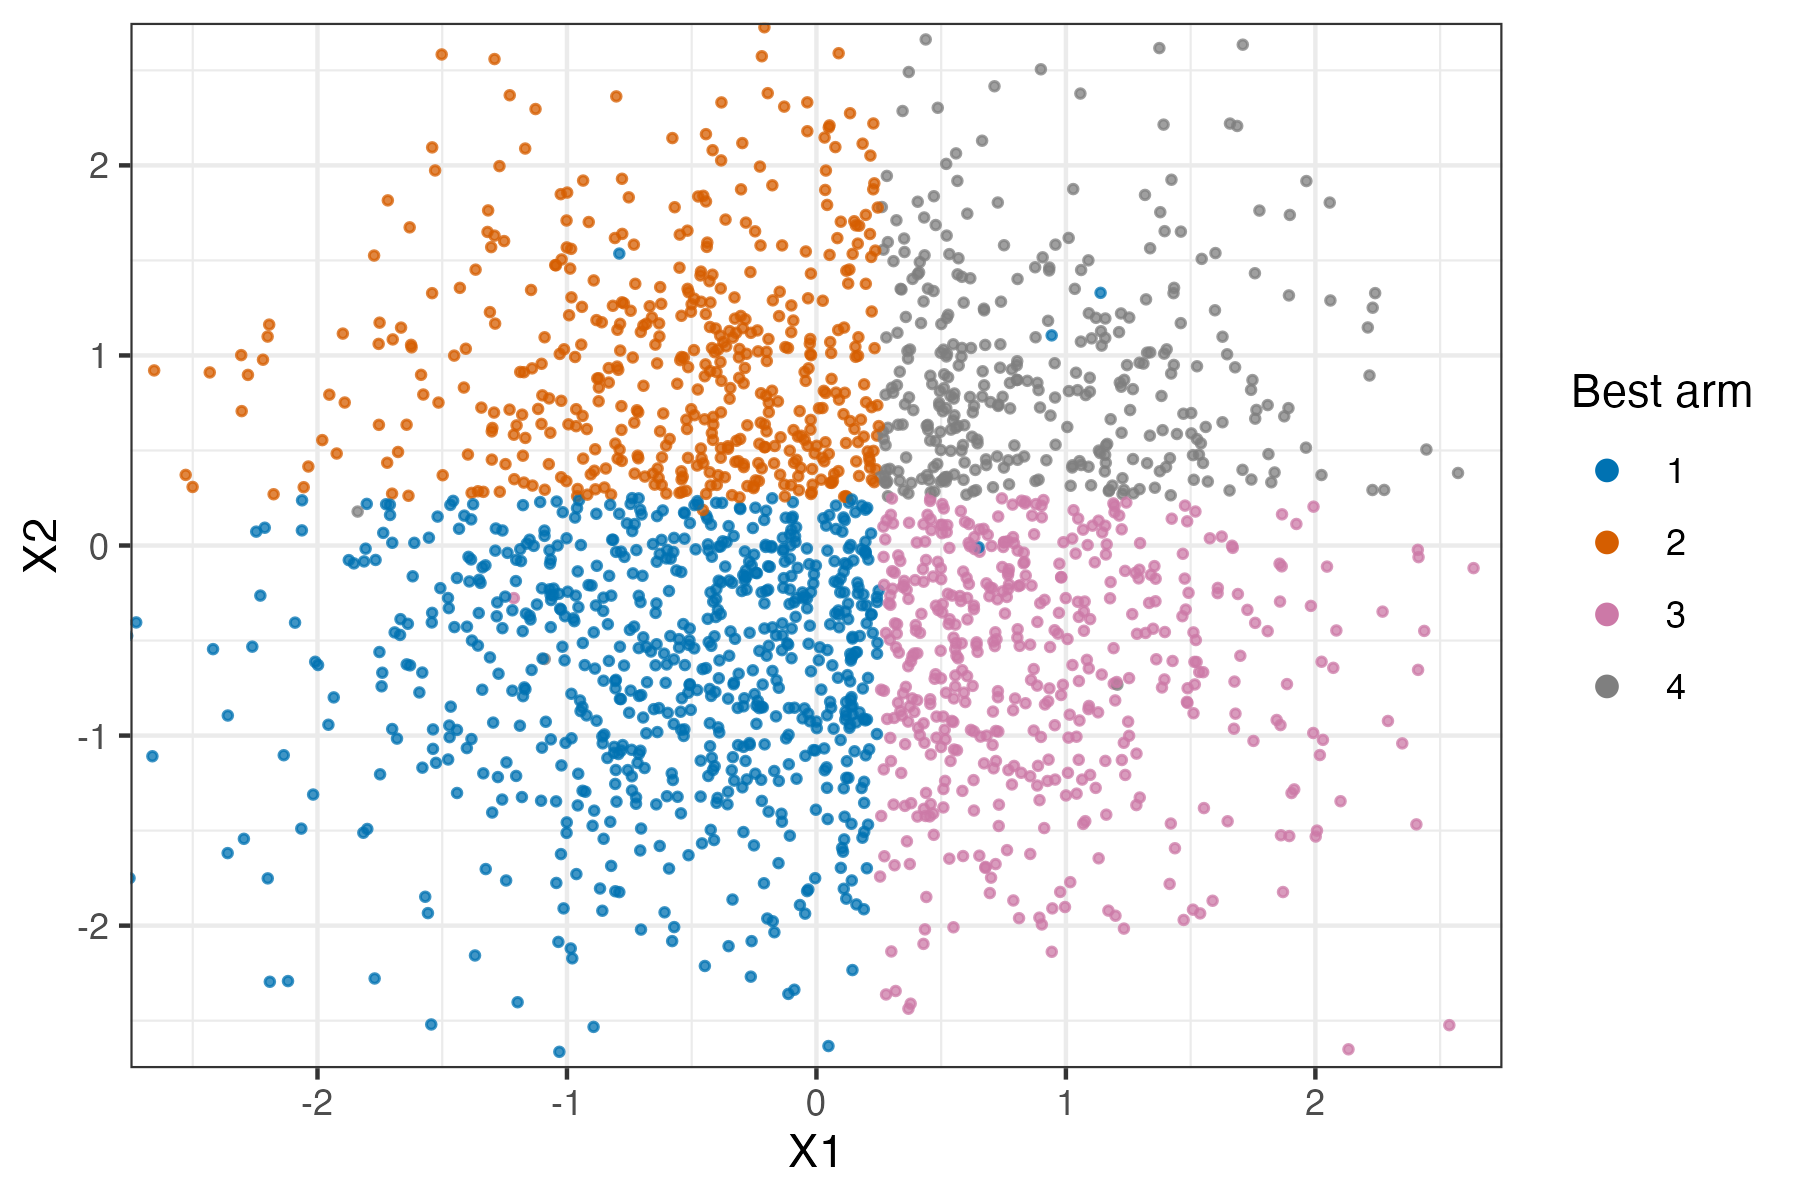
\includegraphics[width=\textwidth]{ tree_dist.png}
      }

\end{frame}


%%%%%NOTE%%%%%
\note{
\scriptsize \singlespacing

%\begin{wideitemize}
%\item xxx
%\end{wideitemize}
}
%-------------------------------------------------------------------------------%
\begin{frame}{Design}

{
      \centering
      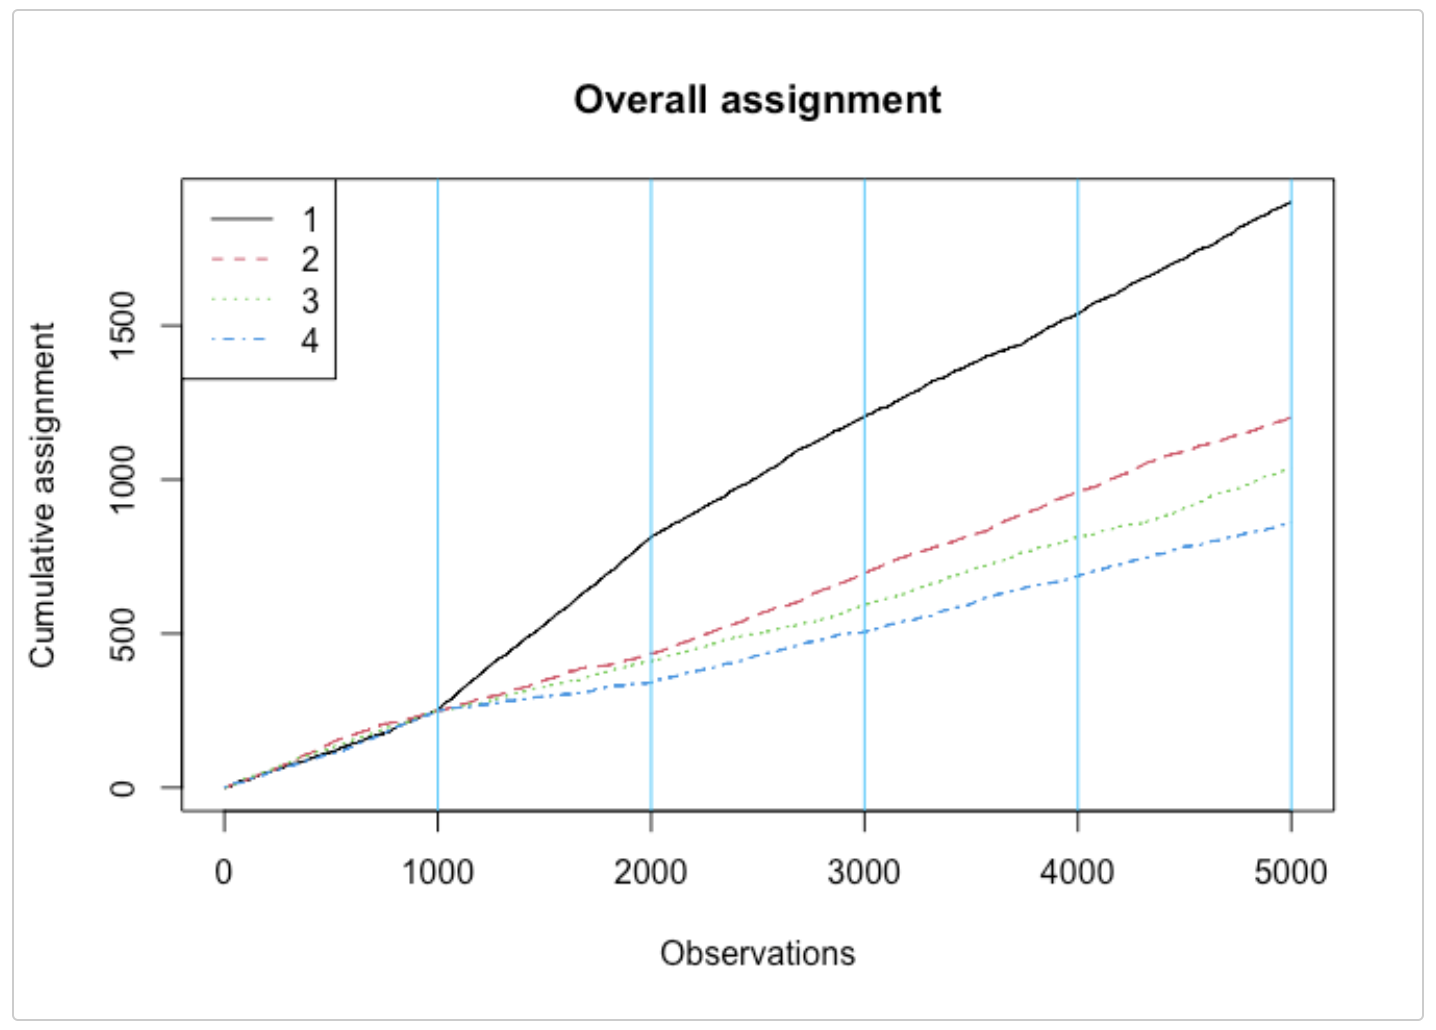
\includegraphics[width=0.95\textwidth]{banditsCIcontextual.png}
      }

\end{frame}


%%%%%NOTE%%%%%
\note{
\scriptsize \singlespacing

%\begin{wideitemize}
%\item xxx
%\end{wideitemize}
}
%-------------------------------------------------------------------------------%
\begin{frame}{Design}

{
      \centering
      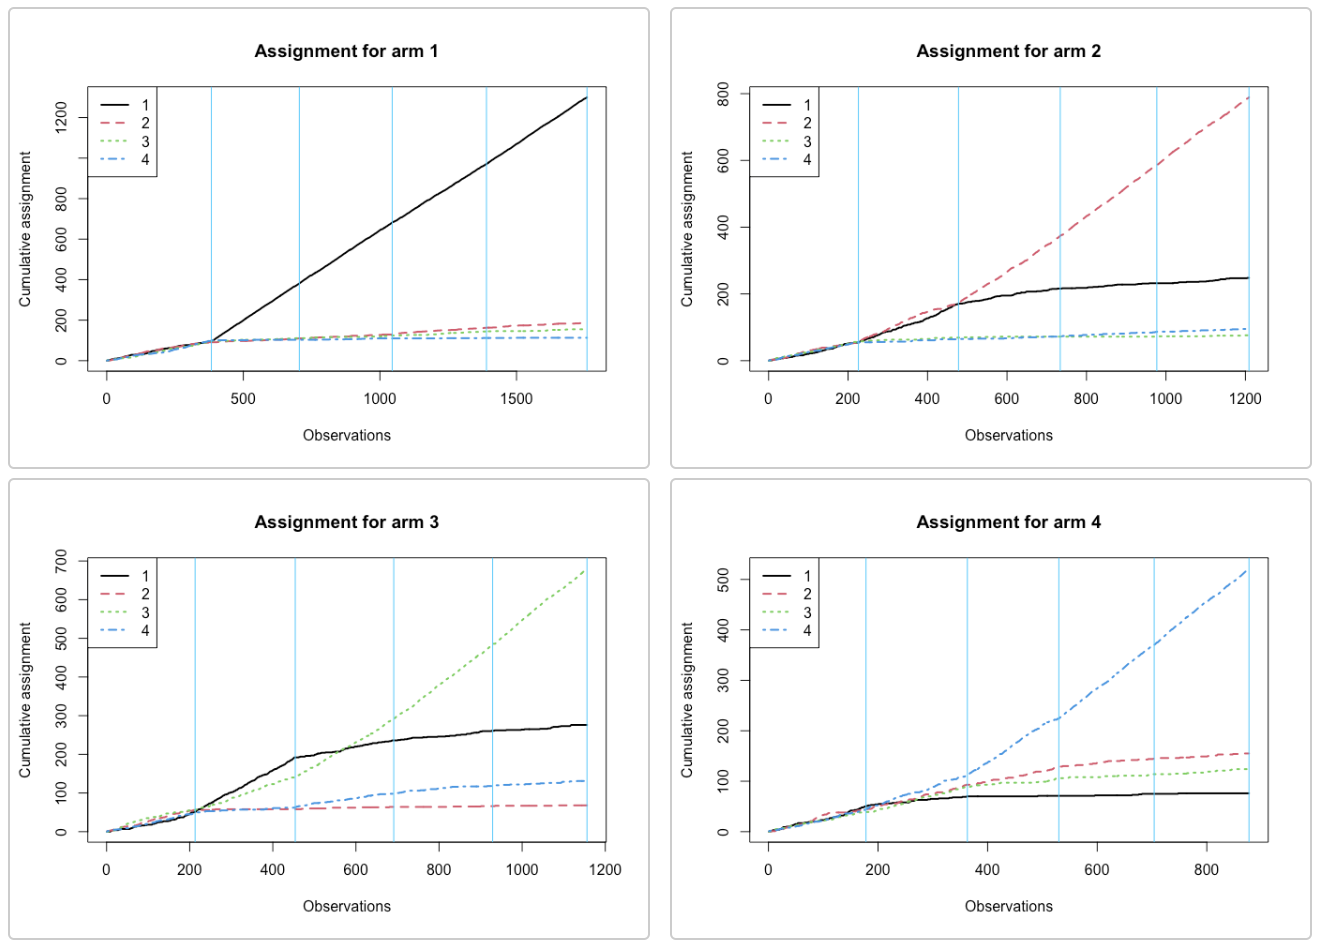
\includegraphics[width=0.95\textwidth]{banditsCIcontextual-sep.png}
      }

\end{frame}


%%%%%NOTE%%%%%
\note{
\scriptsize \singlespacing

%\begin{wideitemize}
%\item xxx
%\end{wideitemize}
}
%-------------------------------------------------------------------------------%
\begin{frame}[label = map]

\begin{wideitemize}
\item \texttt{banditsCI} \url{https://doi.org/10.5281/zenodo.10516416}
\item Applications
\begin{itemize}
\item \hyperlink{vcf}{\beamerbutton{Application I: Vaccine hesitancy}}
\item \hyperlink{misinfo}{\beamerbutton{Application II: Online misinformation}}
\end{itemize}
\item Methods
\begin{itemize}
\item \hyperlink{ts}{\beamerbutton{Algorithms}}
\item \hyperlink{debias}{\beamerbutton{De-biasing and estimation}}
\item \hyperlink{contextualrecs}{\beamerbutton{Contextual recommendation procedures}}
\end{itemize}
\end{wideitemize}

\end{frame}
%-------------------------------------------------------------------------------%
\begin{frame}

\centering{
\texttt{mollyow@uchicago.edu}

\texttt{mollyow.github.io}
}

\end{frame}
%-------------------------------------------------------------------------------%
\algrenewcommand\alglinenumber[1]{\tiny #1:}
\begin{frame}[label=ts]
%\scriptsize
%We suppose that $K$ arms have unknown success rates $\theta_1, \dots, \theta_w$, following their respective Bernoulli distributions, with likelihoods
%\[f_{X_1|\Theta_1}(x_1|\theta_1),\dots, f_{X_w|\Theta_w}(x_w|\theta_w).\]
%Posteriors follow Beta distributions with parameters $\alpha_{w,t}, \beta_{w,t}$. 

\begin{framed}
%\begin{adjustbox}{width = \textwidth, totalheight=\textheight-65pt}
\begin{minipage}{\textwidth}
\tiny
\vspace{-2.5 em}
\begin{algorithm}[H]
%\tiny
\fontsize{5}{6}\selectfont
    \caption{Batch-wise Bernoulli Thompson sampling}
    \label{algg:ts}
 $K$ arms have unknown success rates, $\theta_1, \dots, \theta_k$, following their respective Bernoulli distributions. Priors take the form of $\textrm{Be}(\alpha_w, \beta_w)$. Batches are size $n$.\\
    \begin{algorithmic}[1]

\State Initialize priors such that $(\alpha_{w,1} =1 , \beta_{w, 1}= 1)$ for $w = 1,\dots, K$.
	      \For{periods $t = 1, \dots, T$:}
		      \State Calculate $e_{w, t} = P\left[\Theta_w = {\max}\{\Theta_1,\dots, \Theta_K \}| (\alpha_{1,t}, \beta_{1, t}), \dots, (\alpha_{K,t} ,\beta_{K, t})  \right]$ for $w = 1,\dots, K$.\Comment{Calculate posterior probability that each arm is best. }
		      \State  Sample $n$ observations, assigning treatment with probabilities $(e_{1, t}, \dots, e_{K, t})$.
		     \For{$w =1, \dots, K$}\Comment{Update posteriors.}
		     	\State $\alpha_{w, t+1} \leftarrow \alpha_{w,t} + \# \text{ successes observed for arm $w$ in period $t$}$ 
		     	\State $\beta_{w, t+1}  \leftarrow \beta_{w,t} + \# \text{ failures observed for arm $w$ in period $t$}$
		     \EndFor
	      \EndFor
	\end{algorithmic}
\end{algorithm}
 \end{minipage}
 \vspace{-0.8 em}
%\end{adjustbox}
\end{framed}
 \vspace{-0.5 em}
 
  \hyperlink{ts-explainer}{\beamerbutton{TS explainer}}

\end{frame}
\note{
\scriptsize \singlespacing
\begin{wideitemize}
%\item the question is how you choose a strategy for selecting $n_t$ arms
\item TS one of the oldest and most widely studied approaches to adaptive design, and, as far as I know, what's being used widely in tech industry\\
$\rightarrow$ explain algorithm
\item TS is a decision-theoretic, heuristic approach: gives you info on what to do next\\
\item NOT guaranteed to pick the best arm $\rightarrow$ but performs well in practice
\item And helps navigate the explore/exploit tradeoff: you get enough information about bad arms to know they're not good
\item then want to spend time figuring out, among good arms, which one is truly best. It performs well on each of the objectives outlined above \textcolor{red}{[citations]}. 
\item for probability each arm is optimal--simulate samples, or calculate by quadrature
\item Repeat until stopping rule: \% prob best, or set num periods
\item This is the standard Bayesian approach. In Susan Athey's lab, we're using a frequentist hybrid, where you estimate the mean and variance, assume a normal distribution, and draw from that, but the treatment assignment probability step is very similar
\end{wideitemize}
}

%-------------------------------------------------------------------------------%
\algrenewcommand\alglinenumber[1]{\tiny #1:}
\begin{frame}[label = ttts]

\begin{framed}
%\begin{adjustbox}{width = \textwidth, totalheight=\textheight-65pt}
\begin{minipage}{\textwidth}
\tiny
\vspace{-2.5 em}
\begin{algorithm}[H]
%\tiny
\fontsize{5}{6}\selectfont
    \caption{Bernoulli top-two Thompson sampling}
    \label{algg:ttts}
    \begin{algorithmic}[1] % The number tells where the line numbering should start
    	\State Set  $\alpha_{w} \leftarrow 1, \ \beta_{w} \leftarrow 1\ \forall w \in \ww$; some $\textrm{B}$ parameter in $(0,1)$. %\aB \leftarrow \y \leftarrow $ empty vector.  
	\Comment{Initialize priors}%, assignment vector, and reward vector. }
    	\For{$i = 1, \dots, T$:}
			\For{$w \in \ww$}
		     \State Sample $\hat \theta_w  \sim \textrm{Beta}\left(\alpha_{w}, \beta_{w} \right)$ \Comment{Sample from posteriors. }
			 \EndFor
		\State $I \leftarrow \argmax_w \theta_2 $
		\State Sample $B\sim \textrm{Bernoulli}(\textrm{B})$
		\If{$B = 1$}
			\State Assign treatment $w_i \leftarrow I$
		\Else
			\Repeat
				\For{$w \in \ww$}
					\State Sample $\hat \theta_w  \sim \textrm{Beta}\left(\alpha_{w}, \beta_{w} \right)$ \Comment{Resample from posteriors. }
					\State $J \leftarrow \argmax_w \hat\theta_w$
			 	\EndFor
			\Until{$J \neq I$}
			\State Assign treatment $w_i \leftarrow J$
		\EndIf
%		\State $\aB \leftarrow [\aB : a_i]$ \Comment{Augment assignment vector.}
%		\State $\y \leftarrow [\y : y_i]$ \Comment{Augment reward vector vector.}
			\State $(\alpha_{w_i}, \beta_{w_i}) \leftarrow (\alpha_{w_i} + \mathbbm{1}\{ y_i = 1\} + 1,  \beta_{w_i} + \mathbbm{1}\{ y_i = 0\})$.  \Comment{Update posterior distribution parameters.}
	\EndFor
    \end{algorithmic}
\end{algorithm}
 \end{minipage}
 \vspace{-0.8 em}
%\end{adjustbox}
\end{framed}
 \vspace{-0.5 em}

  \hyperlink{ttts-explainer}{\beamerbutton{TTTS explainer}}
\end{frame}


%%%%%NOTE%%%%%
\note{
\scriptsize \singlespacing

%\begin{wideitemize}
%\item xxx
%\end{wideitemize}
}
%-------------------------------------------------------------------------------%
\begin{frame}[label=cats]{}
\begin{framed}
\begin{minipage}{\textwidth}
\tiny
\vspace{-2.5 em}

\begin{algorithm}[H]
\fontsize{5}{6}\selectfont
    \caption{Control-augmented Thompson sampling}
    \label{algg:cats}
     Suppose some $K$ arms have some unknown success rates, $\theta_1, \dots, \theta_k$, following their respective Bernoulli distributions. Priors take the form of $\textrm{Be}(\alpha_w, \beta_w)$. Let batches be of size $n$.\\
    \begin{algorithmic}[1]

	\State  Let $C$ index the control arm. 
	Initialize priors such that $(\alpha_{w,1} =1 , \beta_{w, 1}= 1)$ for $w \neq C$.
	      \For{periods $t = 1, \dots, T$:}
	      \For{$w \neq C$}
		     \State Calculate $e_{w, t} = P\left[\Theta_w = {\max}\{\Theta_1,\dots, \Theta_K \}| (\alpha_{1,t}, \beta_{1, t}), \dots, (\alpha_{K,t} ,\beta_{K, t})  \right]$ for $w = 1,\dots, K$.\Comment{Calculate posterior probability that each arm is best. }
		\EndFor
		      \State  $b \leftarrow \underset{w}{\argmax} \ p_{w, t} $ \Comment{Retrieve the ``current best arm''\dots}
		      \State $d \leftarrow n_{b, t} - n_{C, t}$ \Comment{\dots and calculate the difference between the cumulative sample assigned to that arm and the control arm.}
		      \State $q \leftarrow \min(\max(d/n, 0), Z_t).$ \Comment{Calculate the proportion of the next batch needed for the control to match the cumulative sample of the ``best'' arm, up to a maximum of $Z_t$ of the batch, where $Z_t \in (0,1)$ may be fixed, or may be data adaptive.}
		      \State  $ \tilde{p}_{C, t} \leftarrow q + R_t*(1-q).$ \Comment{Calculate the probability of assignment to the control condition, a combination of the allocation to match the cumulative sample of the control to the current best arm, and $R_t$ of the remaining probability, for $R_t \in (0,1)$. This value may be fixed, or may also be data adaptive}
		      \For{$w \neq C$}
		      	\State $\tilde{p}_{w, t} \leftarrow p_{w, t}* (1-R_t)*(1-q) $ \Comment{Calculate the probability of assignment to the treatment arms, according to their posterior probabilities, scaled to the remaining sampling probability.}
			\EndFor
		      \State Sample $n$ observations, assigning treatment with probabilities $(\tilde{p}_{1, t}, \dots,\tilde{p}_{C, t}, \dots, \tilde{p}_{W, t} )$.
		      \For{$w \neq C$}\Comment{Update posteriors.}
		     	\State $\alpha_{w, t+1} \leftarrow \alpha_{w,t} + \# \text{ successes observed for arm $w$ in period $t$}$ 
		     	\State $\beta_{w, t+1}  \leftarrow \beta_{w,t} + \# \text{ failures observed for arm $w$ in period $t$}$
		     \EndFor
	      \EndFor
    \end{algorithmic}
\end{algorithm}
 \end{minipage}
 \vspace{-0.8 em}
%\end{adjustbox}
\end{framed}
 \vspace{-0.5 em}
\normalsize
\hyperlink{designcontrol}{\beamerbutton{design overview}}
\end{frame}

%-------------------------------------------------------------------------------%



\begin{frame}[label=bblts]%{Batch-wise balanced linear Thompson sampling}
\begin{framed}
%\begin{adjustbox}{width = \textwidth, totalheight=\textheight-65pt}
\begin{minipage}{\textwidth}
\tiny
\vspace{-2.5 em}
\begin{algorithm}[H]
%\tiny
\fontsize{5}{6}\selectfont
    \caption{Batch-wise balanced linear Thompson sampling}
    \label{algg:bblts}
    \begin{algorithmic}[1] % The number tells where the line numbering should start
    	\State$\Xi \leftarrow$ empty matrix; $\X \leftarrow$ empty matrix; $\y \leftarrow$ empty vector. %for $w \in \ww$. 
	\Comment{Initialize weight matrix, treatment-augmented covariate matrix, and reward vector.  
	}
    	\For{$i = 1, \dots, N$}
		\If{$i \in \mathcal{I}_1$}
			 \State $e_{w} \leftarrow \frac{1 }{|\ww| } \ \ \forall w \in \ww $ \Comment{In first batch, assign treatment uniformly at random.}
		\ElsIf{$i \in \mathcal{I}_b$ for $b = 2, \dots, B$}
			\If{$i$ is the first observation in $\mathcal{I}_b$} \Comment{Update estimates of coefficient vector and variance matrix, using ridge regression with determined penalization.}

				\State $B \leftarrow \X^\top \Xi \X + \lambda^{CV} \mathbf{I}$  
				\State $\hat\theta \leftarrow B^{-1} \X^\top \Xi y$
				\State $\hat\V[\hat\theta] \leftarrow B^{-1} \left(\left( \y - \X^\top\hat\theta \right)^\top \Xi \left( \y - \X^\top\hat\theta \right)\right)$
			\EndIf
			\For{$m = 1, \dots, M$}
				\State Sample $\tilde \theta^{(m)}  \sim \mathcal{N}\left(\hat\theta, \hat\V[\hat\theta] \right)$
			 \EndFor
				\State $q_w \leftarrow \frac{1}{M} \sum_{m=1}^M 1\left\{ w = \underset{w}{\argmax} \{ x_{[1]i}^\top \tilde \theta ^{(m)}, \dots, x_{[|\ww|]i}^\top\tilde \theta^{(m)} \}  \right\}$ \Comment{ Compute TS probabilities based on observed context.}
     			\State $\tilde{q}_w =\max\left\{q_w, p\right\}\ \ \forall w \in \ww$ \Comment{Impose probability floors,}
			\State $u_{\textrm{total}} = \sum_w \tilde{q}_w - 1$ \Comment{ and rescale. }
			\State $u_{w} = \tilde{q}_w - p \ \ \forall w \in \ww$
			\State $ c = u_{\textrm{total}} / \left( \sum_w u_{w} \right)$
			\State $e_w = \tilde{q}_w -c*u_{w} \ \ \forall w \in \ww$
		\EndIf
		\State Assign $w_i \sim \textrm{Multinom}( e_{1}, \dots,  e_{|\ww|} )$ \Comment{Assign treatment.}
		\State $\xi_i \leftarrow \frac{ 1 }{e_{w_i}}$ \Comment{Record inverse probability weights based on realized assignment.}
		\State $\Xi \leftarrow \diag \left(\Xi, \xi_i\right)$ \Comment{Augment weight matrix.}
		\State $\X \leftarrow [\X:x_{[w_i]i}^\top]$ \Comment{Augment covariate matrix.}
		\State $\y \leftarrow  [\y: y_i]$ \Comment{Augment reward vector.}
	\EndFor
    \end{algorithmic}
\end{algorithm}
 \end{minipage}
 \vspace{-0.8 em}
%\end{adjustbox}
\end{framed}
 \vspace{-0.5 em}
% \hyperlink{designend}{\beamerbutton{design overview}}
 \hyperlink{designend2}{\beamerbutton{learning design}}
  \hyperlink{map}{\beamerbutton{navigation}}
\end{frame}


%-------------------------------------------------------------------------------%
\begin{frame}[label = htbias]{Finite-n unbiasedness of the Horvitz-Thompson estimator}

\begin{columns}
\tiny
\setlength{\abovedisplayskip}{5pt}
\setlength{\belowdisplayskip}{0pt}
\setlength{\abovedisplayshortskip}{0pt}
\setlength{\belowdisplayshortskip}{0pt}
    \begin{column}{0.48\textwidth}
Under the potential outcomes framework: 
\begin{align*}
\E\left[ \hat{\theta}_w^{HT} \right]  %& = \E\left[ Y_i(w)\right]
& =\frac 1 N \sum_{i = 1}^N Y_i (w). 
\end{align*}
We require only independence of potential outcomes and treatment conditional on history, $Y_i(w) \independent W_i | S_i$, which is given by the experimental design.  
\begin{align*}
\E\left[ \hat{\theta}_w^{HT} \right] & = \E\left[ \frac 1 N \sum_{i=1}^N Y_{i} \frac{ \mathbbm{1} \{W_i = w \}  }{ e_{i}(w;S_i) }\right]\\
& = \frac 1 N \sum_{i=1}^N \E\left[  Y_{i} \frac{ \mathbbm{1} \{W_i = w \}  }{ e_{i}(w;S_i) }\right].
\intertext{Considering the $i$\textsuperscript{th} unit, by the Law of Iterated Expectations,}
\E\left[  Y_{i} \frac{ \mathbbm{1} \{W_i = w \}  }{ e_{i}(w;S_i) } \right]  & = \E\left[ \E\left[ Y_{i} \frac{ \mathbbm{1} \{W_i = w \}  }{ e_{i}(w;S_i) } \biggr\rvert S_i\right] \right] 
\end{align*}
Taking the interior term, $ \E\left[ Y_{i} \frac{ \mathbbm{1} \{W_i = w \}  }{ e_{i}(w;S_i) } \biggr\rvert S_i\right]$, 
by definition, 
\vskip 1 cm
\normalsize
%\hyperlink{debias}{\beamerbutton{de-biasing}}
\hyperlink{htestimator}{\beamerbutton{HT estimator}} \hyperlink{debiasend}{\beamerbutton{HT toy example}}
\hyperlink{map}{\beamerbutton{navigation}}
    \end{column}
    \begin{column}{0.48\textwidth}
\tiny
\begin{align*}
&  = \E\left[  \frac{ Y_{i} \mathbbm{1} \{W_i = w \}  }{\Pr[ W_i = w | S_i]  } \biggr\rvert S_i \right]
\intertext{By the potential outcomes model,}
&  = \E\left[ Y_{i}(w) \times \frac{ \mathbbm{1} \{W_i = w \}  }{\Pr[ W_i = w | S_i]  } \biggr\rvert S_i \right]
\intertext{And because $Y_i \independent W_i | S_i$, }
&  = \E\left[   Y_{i}(w) | S_i\right] \times \E\left[ \frac{\mathbbm{1} \{W_i = w \}  }{\Pr[ W_i = w | S_i]  } \biggr\rvert S_i \right]\\
&  = \E\left[   Y_{i}(w) | S_i\right] \times  \frac{ \E\left[ \mathbbm{1} \{W_i = w \} | S_i\right] }{\Pr[ W_i = w | S_i]  } \\
&  = \E\left[   Y_{i}(w) | S_i\right] \times  \frac{ \Pr[ W_i = w | S_i] }{\Pr[ W_i = w | S_i]  } \\
&  = \E\left[   Y_{i}(w) | S_i\right]. 
\intertext{Then returning to the Law of Iterated Expectations from above,}
 \E\left[  Y_{i} \frac{ \mathbbm{1} \{W_i = w \}  }{ e_{i}(w;S_i) } \right] &   = \E\left[ \E\left[ Y_i(w) | S_i\right] \right]  = \E\left[ Y_i(w)\right]. 
\end{align*}
\end{column}
\end{columns}

\end{frame}


%%%%%NOTE%%%%%
\note{
\scriptsize \singlespacing

\begin{wideitemize}
\item n and y are correlated, but this is not a ratio estimator, which is why it works
\item Variance...less straightforward
\item \textcolor{Contrast2}{[Finite sample version; include ref for iid? ]}
\item \textcolor{Contrast2}{[Variance?]}
\end{wideitemize}
}
%-------------------------------------------------------------------------------%
\begin{transitionframe}

  \begin{center}
    { \Large \textcolor{white}{De-biasing and estimation}}
  \end{center}
\vfill 

\hyperlink{map}{\beamerbutton{navigation}}
\hypertarget{debias}{}

\end{transitionframe}


%%%%%NOTE%%%%%
\note{
\scriptsize \singlespacing

%\begin{wideitemize}
%\item xxx
%\end{wideitemize}
}
%-------------------------------------------------------------------------------%
\begin{frame}[label = bias0]{Bias and adaptively collected data}

\begin{wideitemize}
\item If we ignore method of data generation and use sample means, adaptively collected data are going to give us estimates that are systematically negatively biased \citep{nie2017adaptively}.
\end{wideitemize}

\end{frame}


%%%%%NOTE%%%%%
\note{
\scriptsize \singlespacing

%\begin{wideitemize}
%\item xxx
%\end{wideitemize}
}
%-------------------------------------------------------------------------------%
\begin{frame}[label = bias1]{Bias in naive estimation w/ adaptive design}

\begin{table}
\centering
\begin{tabular}{l | C{1cm}C{1cm} }
Treatments
& \includegraphics[width = 1cm]{\figpath tv-ad.png} & 
\includegraphics[width = 1cm]{\figpath tv-ad.png}  \\ 
&  \large \textbf A & \large \textbf B \\
\begin{tabular}{@{}c@{}}(Unknown) \\ mean response\end{tabular} %& $\theta_A$ & $\theta_B$\\
& 0.5 & 0.5  \end{tabular}
\end{table}

\textbf{Toy example}\pause
\begin{wideitemize}
\item \textbf{Period 1:} Assign \textbf{one subject each} to treatment A, treatment B.\pause
\item[$\rightarrow$] Observe data.\pause
\item \textbf{Period 2:} Assign treatment probabilistically to \textbf{one subject} using Thompson sampling. \pause
\item[$\rightarrow$]  Three subjects total, two periods. Estimate sample means. 
\end{wideitemize}
\end{frame}


%%%%%NOTE%%%%%
\note{
\scriptsize \singlespacing

\begin{wideitemize}
\item \textcolor{cyan}{Need less technical motivation, and explanation of toy experiment}
\end{wideitemize}
}

%-------------------------------------------------------------------------------%

\begin{frame}[label = bias2]{Bias in naive estimation w/ adaptive design: one realized experiment}

\begin{table}
\centering
\begin{tabular}{l | C{2cm}C{2cm} }
Treatments
& \includegraphics[width = 1cm]{\figpath tv-ad.png} & 
\includegraphics[width = 1cm]{\figpath tv-ad.png}  \\ 
\vspace{4pt} &  \large \textbf A & \large \textbf B \\ \pause
\textbf{Period 1} & & \\
- sample & A & B\\ \pause
- outcome \vspace{4pt} & 1 & 0 \\ \pause
- posterior distributions \vspace{4pt} & $\textrm{Be}(2,1)$ & $\textrm{Be}(1,2)$ \\ \pause

\textcolor{structure}{Sampling probability}  \vspace{4pt} & \textcolor{structure}{5/6} & \textcolor{structure}{1/6}  \\ \pause

 \textbf{Period 2} & & \\ 
- sample & A & -\\ \pause
- outcome \vspace{4pt} & 0 & -  \pause
\\
\hline 
\textbf{Sample mean}  & 0.5 & 0  \\
\end{tabular}
\end{table}

\end{frame}


%%%%%NOTE%%%%%
\note{
\scriptsize \singlespacing

%\begin{wideitemize}
%\item xxx
%\end{wideitemize}
}

%-------------------------------------------------------------------------------%

\setlength{\tabcolsep}{1.3pt}
\begin{frame}[label = bias3]{Bias in naive estimation w/ adaptive design: all paths}
\begin{overprint}

\uncover<7->{After observing three outcomes, bias is negative. }

\vspace{15 pt}
\input{\figpath toy-example.tex}\\

\vspace{-15pt}
\begin{overlayarea}{\textwidth}{0.25\textheight}

\only<7>{ \small
\begin{align*}
\phantom{\E\left[ \hat{\theta}_w \right] \& = \sum_{ s } \hat{\theta}_w | s  \cdot P\left( s \right)}  \\
\phantom{\& \approx 0.458}
\end{align*} 
}

\only<8-9>{ \small
\begin{align*}
\E\left[ \hat{\theta}_w \right] & = \sum_{ s } \hat{\theta}_w | s  \cdot \Pr [s]  \\
& \approx 0.458
\end{align*} }
\uncover<9>{ ($S_i$ is a state, defined by the history of treatment and outcomes.) }

\only<10>{Why? Lower probability of sampling from an arm if it performs poorly in the first period. }

\vspace{10 pt}

%\hyperlink<10>{bias0}{\beamerbutton{Back to main slides}}
\end{overlayarea}
\end{overprint}

\end{frame}

\setlength{\tabcolsep}{6pt}
%%%%%NOTE%%%%%
\note{
\scriptsize \singlespacing

\begin{wideitemize}
\item \textcolor{Cyan}{keep pushing motivation}
\item These are all of the ways that our experiment could possible have played out
\item Pr[s] is the probability that we ended up in that state of the world--note that it's not equal! This is because of the unequal sampling probability, conditional on observed response
\end{wideitemize}
}

%-------------------------------------------------------------------------------%

%%%%NOTE%%%%%
\note{
\scriptsize \singlespacing
\textcolor{structure}{optionally include...}//
Winner's curse:
\begin{wideitemize}
\item Indexing over ARM and then ROUND
\item Calculating for $X_1$, same for $X_2$
\item When it does well in first round, probability of second round weighted up; when poorly, weighted down
\item Note that we're mechanically selecting on the DV
\end{wideitemize}
}
%-------------------------------------------------------------------------------%

\begin{frame}{We can de-bias with weighting estimators}

Inverse Probability Weighting estimation \citep{horvitz1952}\\
\vspace{10pt}
\hspace{5pt}
%For treatment $W_i$, define $e_i(w;S_i) =  \Pr[W_i = w|S_i].$\pause
\begin{align*}
 \hat{\theta}_w^{HT} & =\frac 1 N \sum_{i=1}^N Y_{i} \frac{ \mathbbm{1} \{W_i = w \}  }{e_{i}(w;S_i) }
\end{align*}
\hspace{5pt} \pause
\vspace{10pt}
\begin{wideitemize}
\item (Conditional on algorithm) $e_i(w;S_i) > 0,\forall  i, w$.\\ \pause
\item Finite-n unbiased \citep{bowden2017unbiased} \hyperlink{htbias}{\beamerbutton{Finite-n unbiasedness}}\pause
\item Drawback: if there is low overlap between policy you want to evaluate, and the assigned policy, high variance. One of the tradeoffs we face with adaptively collected data. \hypertarget<3>{htestimator}{}
\end{wideitemize}

\end{frame}
%%%%%NOTE%%%%%
\note{
\scriptsize \singlespacing

\begin{wideitemize}
\item HT: we're taking into account the unequal assignment probabilities
\item drawback of HT: potentially large variance
\begin{wideitemize} \scriptsize
\item[$\rightarrow$] but hopefully, this value is large with respect to the best arm, and so the variance is small
\end{wideitemize}
%\item Some ways to account for bias in design/estimation, but just using naive estimates, can get lower RMSE for best arm in some cases
\item Other estimators are possible, but consistency is design-dependent: 
unless probability of sampling each arm is strictly greater than zero for all time periods, %$\Pr(n_w\to \infty) = 1$, 
there exists no uniformly consistent estimator of $\theta_w$ for all $k$
\item Time trends: probability of being sampled is correlated with underlaying trend
\end{wideitemize}
}
%-------------------------------------------------------------------------------%

\begin{frame}[label= ht_example]{Estimation with Inverse Probability Weighting}

\begin{align*}
 \hat{\theta}_w^{HT} & =\frac 1 N \sum_{i=1}^N Y_{i} \frac{ \mathbbm{1} \{W_i = w \}  }{e_{i}(w;S_i) }
\end{align*}
\pause

In our example\dots
\begin{align*}
 \hat{\theta}_A^{HT} & =\frac 1 3 \left[  1 \times \frac{ \mathbbm{1} \{W_i = A \}  }{1/2 } + 0 \times \frac{ \mathbbm{1} \{W_i = A \}  }{5/6 } \right]\\
 & = \frac 2 3
\end{align*}


\end{frame}


%%%%%NOTE%%%%%
\note{
\scriptsize \singlespacing

%\begin{wideitemize}
%\item xxx
%\end{wideitemize}
}

%-------------------------------------------------------------------------------%


\setlength{\tabcolsep}{1.3pt}
\begin{frame}[label = debias]{De-biasing estimation: all paths}

%\textcolor{white}{After observing three outcomes, bias is negative. }

\vspace{15 pt}
\input{\figpath toy-example-debiased.tex}

\onslide<3->
\begin{align*}
\textcolor{Contrast2}{\E\left[ \hat{\theta}^{HT}_w \right]} & \textcolor{Contrast2}{ = \sum_{ s } \hat{\theta}^{HT}_w | s  \cdot \Pr[ s ]}  \\
& \textcolor{Contrast2}{= 0.5}
\end{align*}
%($S_i$ is a state, defined by the history of treatment and outcomes.) \\
\vfill

\hyperlink{htbias}{\beamerbutton{HT unbiased}} \hypertarget<3>{debiasend}{}
\end{frame}

\setlength{\tabcolsep}{6pt}
%%%%%NOTE%%%%%
\note{
\scriptsize \singlespacing

%\begin{wideitemize}
%\item xxx
%\end{wideitemize}
}

%-------------------------------------------------------------------------------%

\begin{frame}{Covariate adjustment: doubly robust estimation}
\small
We can also consider inverse probability weighting augmented by covariate adjustment. 
\begin{overprint}
\[
    \hat{\theta}_w^{DR} =\frac 1 N  \sum_{i=1}^N \only<2>{\textcolor{Contrast1}}{\underbrace{\hat{\E}[Y_i | W_i = w, X_i]}_\text{estimated outcome model}}+\frac{1}{N} \sum_{i=1}^N  \underbrace{\frac{ \mathbbm{1} \{W_i = w \} \left( Y_i - \only<2>{\textcolor{Contrast1}}{\hat{\E}[Y_i | W_i = w, X_i]} \right) }{ \only<3>{\textcolor{Contrast2}}{ e_i(w;s)} }}_\text{residual bias correction}
\]

\begin{overlayarea}{\textwidth}{0.25\textheight}

\only<2>{
\begin{wideitemize}
  \item We can use regression--or machine-learning methods--for estimation of the \textcolor{Contrast1}{outcome model},
  \item[] \phantom{or of the \textcolor{Contrast2}{weights}. } 
\end{wideitemize}
	   }
\only<3>{
\begin{wideitemize} 
  \item We can use regression--or machine-learning methods--for estimation of the \textcolor{black}{outcome model}.
%  \item or of the \textcolor{Contrast2}{weights}. 
\end{wideitemize}
  }
\end{overlayarea}
\end{overprint}
\end{frame}


%%%%%NOTE%%%%%
\note{
\scriptsize \singlespacing

\begin{wideitemize}
\item Doubly-robust estimation: HR ``a doubly robust estimator consistently estimates the causal effect if at least one of the
two models is correct (and one need not know which of the two models is correct).''; it is efficient if both are correctly specified and data is i.i.d. 
\item This is the simple model of AIPTW estimator, but could use anything with the DR property, e.g., TMLE
\item Conditional means model (any well-behaved prediction will do), improves efficiency;  could be something like a regression estimate, a regularized model with interactions between treatment and covariates, random forest, etc. 
\item even if exposure is known, we can estimate it to capture chance imbalances in covariate distribution among groups \textcolor{Contrast2}{[Hirano-Imbens-Ridder result]}. 
%\item \texttt{lim[n] n*Var[Q-hat[w]] = lim[n] 1/n sum[i to n] (1/e[i][w] - 1) * (mu-hat[i] - Q[w])\^2 + 1/e[i][w] * Var(Y[w])}\\
\item \textcolor{Contrast2}{So as long as your \texttt{mu-hat[i]} model is sensible, you can decrease the first term in the asymptotic variance.}
\end{wideitemize}
}


%-------------------------------------------------------------------------------%
\backupbegin
%-------------------------------------------------------------------------------%

\begin{frame}[allowframebreaks]{References}
    \bibliographystyle{apalike}
    \bibliography{\plscbibpath}
\end{frame}
%-------------------------------------------------------------------------------%
\backupend
\end{document}
%-------------------------------------------------------------------------------%

%%% [[TEMPLATE]] %%%
\begin{frame}{Frametitle}

%\begin{wideitemize}
%\item xxx
%\end{wideitemize}

\end{frame}


%%%%%NOTE%%%%%
\note{
\scriptsize \singlespacing

%\begin{wideitemize}
%\item xxx
%\end{wideitemize}
}
%-------------------------------------------------------------------------------%